\documentclass[a4paper,11pt]{book}
%\documentclass[a4paper,twoside,11pt,titlepage]{book}
\usepackage{listings}
\usepackage[utf8]{inputenc}
\usepackage[spanish]{babel}

% \usepackage[style=list, number=none]{glossary} %
%\usepackage{titlesec}
%\usepackage{pailatino}

\decimalpoint
\usepackage{dcolumn}
\newcolumntype{.}{D{.}{\esperiod}{-1}}
\makeatletter
\addto\shorthandsspanish{\let\esperiod\es@period@code}
\makeatother


%\usepackage[chapter]{algorithm}
\RequirePackage{verbatim}
%\RequirePackage[Glenn]{fncychap}
\usepackage{fancyhdr}
\usepackage{graphicx}
\usepackage{afterpage}

\usepackage{longtable}

\usepackage[colorlinks=true,linkcolor=black,citecolor=blue,urlcolor=blue]{hyperref} %referencia

\usepackage{float}
\usepackage{amsmath}
\usepackage{url}


% ********************************************************************
% Re-usable information
% ********************************************************************

\newcommand{\myTitle}{Aplicaciones prácticas del análisis de componentes principales dinámicos generalizados (Generalized Dynamic Principal Components)}
\newcommand{\myDegree}{Doble Grado en Ingeniería Informática y Matemáticas }
\newcommand{\myName}{Anabel Gómez Ríos}
\newcommand{\myProf}{Héctor E. Pomares Cintas}
%\newcommand{\myOtherProf}{Put name here}
%\newcommand{\mySupervisor}{Put name here\xspace}
\newcommand{\myFaculty}{Escuela Técnica Superior de Ingenierías Informática y de Telecomunicación, Facultad de Ciencias}
\newcommand{\myFacultyShort}{}
\newcommand{\myDepartment}{}
\newcommand{\myUni}{\protect{Universidad de Granada}}
\newcommand{\myLocation}{Granada}
\newcommand{\myTime}{Septiembre, 2016}
\newcommand{\myVersion}{Version 0.1}


\hypersetup{
pdfauthor = {\myName (anabelgrios (en) correo (punto) ugr (punto) es)},
pdftitle = {\myTitle},
pdfsubject = {},
pdfkeywords = {palabra_clave1, palabra_clave2, palabra_clave3, ...},
pdfcreator = {LaTeX con el paquete ....},
pdfproducer = {pdflatex}
}

% ********************************************************************
%\hyphenation{}


%\usepackage{doxygen/doxygen}
%\usepackage{pdfpages}
\usepackage{url}
\usepackage{colortbl,longtable}
\usepackage[stable]{footmisc}
\usepackage{amsthm}
%\usepackage{index}
\usepackage{amssymb}

%\makeindex
%\usepackage[style=long, cols=2,border=plain,toc=true,number=none]{glossary}
% \makeglossary

% Definición de comandos que me son útiles:
%\renewcommand{\indexname}{Índice alfabético}
%\renewcommand{\glossaryname}{Glosario}

\pagestyle{fancy}
\fancyhf{}
\fancyhead[LO]{\leftmark}
\fancyhead[RE]{\rightmark}
\fancyhead[RO,LE]{\textbf{\thepage}}
\renewcommand{\chaptermark}[1]{\markboth{\textbf{#1}}{}}
\renewcommand{\sectionmark}[1]{\markright{\textbf{\thesection. #1}}}

\setlength{\headheight}{1.5\headheight}

\newcommand{\HRule}{\rule{\linewidth}{0.5mm}}
%Definimos los tipos teorema, ejemplo y definición podremos usar estos tipos
%simplemente poniendo \begin{teorema} \end{teorema} ...
\newtheorem{ejemplo}{Ejemplo}[chapter]
\theoremstyle{plain}
\newtheorem{teorema}{Teorema}[chapter]
\newtheorem{lema}[teorema]{Lema}
\newtheorem{proposicion}[teorema]{Proposición}
\newtheorem{corolario}[teorema]{Corolario}

% Definición de estilo de definición



\newtheoremstyle{definition_wo_parentheses}
  {\topsep}% measure of space to leave above the theorem. E.g.: 3pt
  {\topsep}% measure of space to leave below the theorem. E.g.: 3pt
  {}% name of font to use in the body of the theorem
  {0pt}% measure of space to indent
  {\bfseries}% name of head font
  {.}% punctuation between head and body
  { }% space after theorem head; " " = normal interword space
  {\thmname{#1}\thmnumber{ #2}\thmnote{ #3}}
  
  
\theoremstyle{definition_wo_parentheses}	
\newtheorem{definicion}{Definición}[chapter]
\newtheorem{nota}{Nota}[chapter]

\definecolor{gray97}{gray}{.97}
\definecolor{gray75}{gray}{.75}
\definecolor{gray45}{gray}{.45}
\definecolor{gray30}{gray}{.94}

\lstset{ frame=Ltb,
     framerule=0.5pt,
     aboveskip=0.5cm,
     framextopmargin=3pt,
     framexbottommargin=3pt,
     framexleftmargin=0.1cm,
     framesep=0pt,
     rulesep=.4pt,
     backgroundcolor=\color{gray97},
     rulesepcolor=\color{black},
     %
     stringstyle=\ttfamily,
     showstringspaces = false,
     basicstyle=\scriptsize\ttfamily,
     commentstyle=\color{gray45},
     keywordstyle=\bfseries,
     %
     numbers=left,
     numbersep=6pt,
     numberstyle=\tiny,
     numberfirstline = false,
     breaklines=true,
   }
 
% minimizar fragmentado de listados
\lstnewenvironment{listing}[1][]
   {\lstset{#1}\pagebreak[0]}{\pagebreak[0]}

\lstdefinestyle{CodigoC}
   {
	basicstyle=\scriptsize,
	frame=single,
	language=C,
	numbers=left
   }
\lstdefinestyle{CodigoC++}
   {
	basicstyle=\small,
	frame=single,
	backgroundcolor=\color{gray30},
	language=C++,
	numbers=left
   }
\lstdefinestyle{CodigoR}
   {
	basicstyle=\small,
	frame=single,
	backgroundcolor=\color{gray30},
	language=R,
	numbers=left
   }
 
\lstdefinestyle{Consola}
   {basicstyle=\scriptsize\bf\ttfamily,
    backgroundcolor=\color{gray30},
    frame=single,
    numbers=none
   }


\newcommand{\bigrule}{\titlerule[0.5mm]}


%Para conseguir que en las páginas en blanco no ponga cabecerass
\makeatletter
\def\clearpage{%
  \ifvmode
    \ifnum \@dbltopnum =\m@ne
      \ifdim \pagetotal <\topskip
        \hbox{}
      \fi
    \fi
  \fi
  \newpage
  \thispagestyle{empty}
  \write\m@ne{}
  \vbox{}
  \penalty -\@Mi
}
\makeatother

\usepackage{pdfpages}
\usepackage{gensymb}
\usepackage{amsfonts}
\usepackage{amsmath}

% Comandos para la escritura 
\newcommand{\abs}[1]{\left\lvert#1\right\rvert}
\newcommand{\norm}[1]{\left\lVert#1\right\rVert}
\newcommand{\var}{\text{var}}
\newcommand{\cov}{\text{cov}}

% Pseudocódigo
\usepackage{algorithm}
\usepackage{algorithmic}

% ****************************************************************
% DOCUMENTO
% ****************************************************************

\begin{document}
\pagenumbering{roman}
\begin{titlepage}

\newlength{\centeroffset}
\setlength{\centeroffset}{-0.5\oddsidemargin}
\addtolength{\centeroffset}{0.5\evensidemargin}
\thispagestyle{empty}

\noindent\hspace*{\centeroffset}\begin{minipage}{\textwidth}

\centering

\includegraphics[width=0.9\textwidth]{imagenes/logo_ugr.jpg}\\[1.4cm]

\textsc{ \Large TRABAJO FIN DE GRADO\\[0.2cm]}
\textsc{ \myDegree }\\[1cm]
% Upper part of the page
% 
% Title
{\Large \bfseries{ \myTitle }\\ }
\noindent\rule[-1ex]{\textwidth}{3pt}\\[3.5ex]
{\large\bfseries}
\end{minipage}

\vspace{2.5cm}
\noindent\hspace*{\centeroffset}\begin{minipage}{\textwidth}
\centering

\textbf{Autor}\\ {\myName}\\[2.5ex]
\textbf{Director}\\
{\myProf}\\[2cm]
\textsc{ \myFaculty }\\
\textsc{---}\\
\myTime
\end{minipage}
%\addtolength{\textwidth}{\centeroffset}
%\vspace{\stretch{2}}
\end{titlepage}



\chapter*{}
%\thispagestyle{empty}
%\cleardoublepage

%\thispagestyle{empty}

\begin{titlepage}
 
 
\setlength{\centeroffset}{-0.5\oddsidemargin}
\addtolength{\centeroffset}{0.5\evensidemargin}
\thispagestyle{empty}

\noindent\hspace*{\centeroffset}\begin{minipage}{\textwidth}

\centering
%
\includegraphics[width=0.9\textwidth]{imagenes/logo_ugr.jpg}\\[1.4cm]

%\textsc{ \Large PROYECTO FIN DE CARRERA\\[0.2cm]}
%\textsc{ INGENIERÍA EN INFORMÁTICA}\\[1cm]
% Upper part of the page
% 

 \vspace{3.3cm}

%si el proyecto tiene logo poner aquí
%
\includegraphics{imagenes/logo.png} 
% \vspace{0.5cm}

% Title

{\Large\bfseries \myTitle \\}
\noindent\rule[-1ex]{\textwidth}{3pt}\\[3.5ex]
%{\large\bfseries Subtítulo del proyecto.\\[4cm]}
\end{minipage}

\vspace{2.5cm}
\noindent\hspace*{\centeroffset}\begin{minipage}{\textwidth}
\centering

\textbf{Autor}\\ { \myName}\\[2.5ex]
\textbf{Director}\\
	{ 	\myProf }\\[2cm]
%
\includegraphics[width=0.15\textwidth]{imagenes/tstc.png}\\[0.1cm]
%\textsc{Depto.}\\
%\textsc{---}\\
%Granada, mes de 201
\end{minipage}
%\addtolength{\textwidth}{\centeroffset}
\vspace{\stretch{2}}

 
\end{titlepage}






\cleardoublepage
\thispagestyle{empty}

\begin{center}
{\large\bfseries \myTitle }\\
\end{center}
\begin{center}	
	\myName \\
\end{center}

%\vspace{0.7cm}
\noindent{\textbf{Palabras clave}: reducción de dimensión, análisis de componentes principales, series temporales, predicción de series temporales, compresión de imágenes.}\\

\vspace{0.7cm}
\noindent{\textbf{Resumen}}\\

En el presente trabajo se expone una nueva forma de reducción de dimensión en el contexto de series temporales dada por Peña y Yohai en \cite{pena16} y una serie de aplicaciones a la misma interesantes en dicho contexto. Para ello, comenzamos hablando del análisis de componentes principales, uno de los métodos más importantes y más conocidos en la reducción de dimensiones de un conjunto de datos, por ser uno de los métodos en los que se basa en análisis de componentes principales dinámicas generalizado o GDPC, por sus siglas en inglés. De esta forma, dedicamos la primera parte del capítulo \ref{ch:matematicas} al estudio del análisis de componentes principales, dando los fundamentos matemáticos y las demostraciones del mismo. Después damos una breve introducción a las series temporales y a los más básicos modelos lineales que hay para modelarlas, ya que serán de utilidad más adelante. La última parte del capítulo \ref{ch:matematicas} se dedica al algoritmo GDPC, dando los pasos de Peña y Yohai para calcular las componentes principales dinámicas que ellos definen y se comenta el análisis de componentes principales de Brillinger, otro de los puntos de partida de Peña y Yohai, dando las principales diferencias y ventajas entre el generalizado y el de Brillinger y el análisis de componentes principales.\\

La segunda parte del trabajo se centra en buscar y probar algunas aplicaciones del GDPC, además de hacer un estudio de los parámetros del mismo que influyen en el tiempo de ejecución. Para esta parte se ha utilizado el paquete en desarrollo en \cite{ezeq}. La primera de las aplicaciones es la compresión de imágenes, y aunque no se pretende dar un método de compresión que mejore los ya existentes (los tiempos de cómputo son muy altos comparando con el algoritmo de compresión JPEG, por ejemplo, y la calidad es peor), sirve para entrar en contacto con el método y llegar a entender mejor su funcionamiento. Las otras dos aplicaciones mostradas y llevadas a cabo sí se pueden utilizar dentro del contexto de series temporales y han resultado ser muy interesantes. La primera de ellas es la búsqueda de patrones periódicos en series temporales periódicas, una práctica llevada a cabo a menudo en análisis de series temporales. Es interesante porque se pueden llegar a conseguir patrones con un preprocesamiento mínimo y automático de la serie original. La última aplicación es la predicción de un determinado número de valores de un conjunto de series temporales. Esta es la aplicación más importante a la que se ha llegado, porque permite predecir valores de un conjunto amplio de series temporales (de hecho, tan grande como se quiera), que es la práctica más común en series temporales, prediciendo valores de un conjunto muy reducido de series: las componentes principales dinámicas. Es decir, lo que se hace es utilizar los modelos existentes para predecir los siguientes valores de las componentes principales dinámicas para después volver hacia atrás con una pequeña modificación del método de reconstrucción de las series originales utilizando las componentes principales dinámicas con las predicciones. Esta aplicación, además, ha resultado dar unos resultados buenos utilizando sólo los modelos lineales más simples para la parte de predicción de nuevos valores.

\cleardoublepage


\thispagestyle{empty}


\begin{center}
{\large\bfseries Generalized Dynamic Principal Components Analysis and its applications}\\
\end{center}
\begin{center}
	\myName	\\
\end{center}

%\vspace{0.7cm}
\noindent{\textbf{Keywords}: dimension reduction, Principal Component Analysis, time series, time series prediction, image compression}\\

\vspace{0.7cm}
\noindent{\textbf{Abstract}}\\

In this work we explain a new way of dimension reduction in the context of time series analysis, given by Peña and Yohai in \cite{pena16}, called Generalized Dynamic Principal Components, or GPDC. Besides, we give differents applications of the GDPC, which are interesting in the context of time series analysis. In order to give and explain this applications, and do a few examples of each one of them, we start explaining the Principal Component Analysis, or PCA, one of the most important and one of the best known procedures in the context of dimension reduction as well as this is one of the procedures in which the Generalized Dynamic Principal Component is based. Therefore, we dedicate the first section of the chapter \ref{ch:matematicas} to study the Principal Component Analysis, given the mathematical fundaments and the proofs of this procedure.\\

Dimension reduction has become, in recent years, in one of the most important problems of the computer science, since every day more information is stored and we need to deal and work with large quantities of data, being required to lost some parts of the information in order to be able to work with it. Principal Component Analysis give us a way to do that. In rough outlines, if we have a data set of $n$ dimensions, PCA searches for a new set of axis, for example $m$ new axis, rotations of the old ones, with $m \leq n$. That way, the data set in the new axis has only $m$ dimensions. The number $m$ can be chosen based on the amount of information we are willing to lose. By intuition, as more correlated are the data, fewer axis, that is, fewer principal components, will be necessary to use.\\

Now, one of the ways of storing larges amounts of data is when we store consecutive values (usually taken in regular time intervals) of a random variable, for example, the number of cars sold in a city every month or the number of deaths in a city every month or every year. There are a lot of possibilities and work with this kind of information help us to predict what is going to happen in short-term. This kind of information stored is called time series and we dedicate the second section of the chapter \ref{ch:matematicas} to introduce the basics of them.\\

Besides, it is also interesting to reduce the dimension of time series because usually several time series are correlated between each other, like the number or car crashes in a city, the number or mortal diseases in the same city and the number of deaths in the same city. When we have a lot of data (for example, suppose we have the three series we just mention since 1700) and a lot of series that are correlated, is better to reduce the dimension and work with reduced data sets. This is the base of the Generalized Dynamic Principal Component, to reduce the dimension in several time series. We dedicate the rest of the chapter \ref{ch:matematicas} to this procedure. We summarize the paper of Peña and Yohai (\cite{pena16}).\\

We focus the second part of this work in searching and testing differents applications of the GDPC, in addition to do a study of what parameters has influence in the time that the procedure takes to finish. We do all the test with a development version of the GPDC given by Ezequiel Smucler in \cite{ezeq}. The first application of the GPDC is in image compression. Although we don't pretend to give a method which beats one that already exists (for example, the time that it takes to compress a image with GPDC is way long that the time that it takes to compress a image with JPEG, and the quality of the resulting image is better with JPEG than with GDPC). However, this application help us to understand completely the procedure of Generalized Dynamic Principal Components and to make contact with the package in R given by Ezequiel Smucler. We develop this application in the second part of chapter \ref{ch:informatica}.\\

The other two applications shown can be used in a time series context and in fact, they have proved to give good results. The second one is searching patterns in periodic time series, which is a practise performed often in time series analysis. This application is interesting because we can find patterns with a minimum and automatic pre-processing of the original time serie, as we will see in the third section of the chapter \ref{ch:informatica}. The last, and most interesting application that we give is the prediction of new values from a given set of time series. This is the most interesting application because it allows to predict $p$ new values from a large set of time series (in fact, it could be as bigger as we want), which is the most commom practise in time series analysis, only predicting $p$ new values of a reduced set of time series: the dynamic principal components. That is, we use the existing models for prediction in order to predict the next $p$ values of every dynamic principal component obtained so we can go back to the original series (plus the $p$ new values predicted) with a small alteration of the method that obtains the reconstructed series, using the dynamic principal components with the $p$ predicted values. This application, furthermore, has proved to give good results even using the simplest lineal models for the prediction of the new values in the dynamic principal components, which could lead us to continue investigating this application.\\

This is one of the future works we give in the chapter \ref{ch:conclusiones}, which closes this work.

\chapter*{}
\thispagestyle{empty}

\noindent\rule[-1ex]{\textwidth}{2pt}\\[4.5ex]

Yo, \textbf{\myName}, alumna de la titulación \myDegree  de la \textbf{\myFaculty  de la \myUni}, con DNI 75929914Z, autorizo la
ubicación de la siguiente copia de mi Trabajo Fin de Grado en la biblioteca de ambos centros para que pueda ser
consultada por las personas que lo deseen.

\vspace{6cm}

\noindent Fdo: \myName

\vspace{2cm}

\begin{flushright}
Granada a 8 de septiembre de 2016.
\end{flushright}


\chapter*{}
\thispagestyle{empty}

\noindent\rule[-1ex]{\textwidth}{2pt}\\[4.5ex]

D. \textbf{ \myProf }, Profesor del Departamento de Arquitectura y Tecnología de los Computadores de la Universidad de Granada.

\vspace{0.5cm}


\textbf{Informa:}

\vspace{0.5cm}

Que el presente trabajo, titulado \textit{\textbf{\myTitle}},
ha sido realizado bajo su supervisión por \textbf{\myName}, y autoriza la defensa de dicho trabajo ante el tribunal
que corresponda.

\vspace{0.5cm}

Y para que conste, expide y firma el presente informe en Granada a 8 de septiembre de 2016.

\vspace{1cm}

\textbf{El director:}

\vspace{5cm}

\noindent \textbf{\myProf}

\chapter*{Agradecimientos}
\thispagestyle{empty}

       \vspace{1cm}


Quería agradecer a la Universidad de Granada y a los profesores de ambas titulaciones por ayudarme a formarme en las dos áreas que siempre he querido. A mi tutor, Héctor Pomares, por ayudarme además a realizar el presente trabajo.\\

Quería agradecer también a mi familia y amigos, sin cuya ayuda y apoyo inestimable no podría haber seguido adelante.


%\frontmatter
\tableofcontents
%\listoffigures
%\listoftables
%
%\mainmatter
%\setlength{\parskip}{5pt}


%\documentclass[11pt,leqno]{book}
%\usepackage[spanish,activeacute]{babel}
%\usepackage[utf8]{inputenc}
%\usepackage{enumerate}
%\usepackage{float}
%\usepackage{gensymb}
%
%\begin{document}


\chapter{Introducción}
\pagenumbering{arabic}
\setcounter{page}{1}

\section{Contextualización}
La reducción de dimensión se ha convertido, desde hace unos años, en uno de los grandes problemas de la informática, al almacenarse cada vez más información y tener que trabajar con grandes cantidades de datos, lo que conlleva tiempos de ejecución inabarcables, haciéndose muchas veces necesario eliminar partes de la información para poder trabajar con ella. Una de las formas de reducir la dimensión de un conjunto de datos es el análisis de componentes principales. A grandes rasgos, si se dispone de un conjunto de datos de $n$ dimensiones, el análisis de componentes principales busca $m$ nuevos ejes, rotación de los originales, con $m \leq n$, de forma que los datos representados en los nuevos ejes tienen sólo $m$ dimensiones. El número de ejes, es decir, de componentes principales, $m$, se puede elegir en función de la cantidad de información que se está dispuesto a perder, ya que se pueden ir eliminando aquellas componentes que menos influyan en los datos. Intuitivamente, cuanto más relacionados estén los datos entre sí, menos componentes principales serán necesarias. Esto es fácil de ver con el siguiente ejemplo: supongamos que disponemos de 10 datos en $\mathbb{R}^2$, todos alineados. Si obtenemos la primera componente principal, que será la línea por la que pasan los datos, y nos quedamos con la representación de los datos en esta línea, sólo tendremos que almacenar una dimensión, y además lo estamos haciendo sin perder información alguna.\\

Ahora, una de las formas en las que se almacena mucha información es cuando se guarda el valor de una variable a lo largo de periodos de tiempo, por ejemplo, el tiempo en una ciudad a lo largo del año, el número de coches vendidos por meses a lo largo de los últimos 15, 20 o 30 años, el número de defunciones en una ciudad o país desde 1900, o la cantidad de contagios de enfermedades al mes por ciudades. Las posibilidades son infinitas y almacenar y trabajar sobre este tipo de información nos ayuda a predecir qué puede pasar sobre un determinado tema a corto plazo. Además, normalmente este tipo de información no es independiente y depende de varios factores. Por ejemplo, el número de defunciones dependerá del número de contagios de distintas enfermedades en la misma ciudad en ese mes, o el consumo de carburante con la cantidad de coches en circulación. Este tipo de información almacenada se llaman series temporales y es de nuevo interesante reducir la dimensión de las mismas con objeto de trabajar mejor sobre ellas. En esto se centra el paper de Daniel Peña y Víctor Yohai, \cite{pena16}, que aquí se aborda y del que se dan varias posibles aplicaciones.


\section{Descripción del problema abordado}



\section{Técnicas y herramientas utilizadas}


\section{Contenido de la memoria y principales fuentes consultadas}



%\end{document}
%
\chapter{Objetivos del trabajo}

Los objetivos previstos inicialmente para este proyecto fueron los siguientes:
\begin{enumerate}
\item Comprender los principios básicos del método \textit{Generalized Dynamic Principal Components (GDPC)} y de los métodos de los que deriva.
\item Aplicar dicho método a compresión de imágenes.
\item Aplicar dicho método a predicción bursátil.
\item Realizar aplicaciones en Brain Computing Interfaces.
\end{enumerate}

El primer y principal objetivo se ha cumplido por completo, entendiendo el análisis de componentes principales dinámicos generalizado. Para ello ha hecho falta buscar y entender también el análisis de componentes principales o PCA, por sus siglas en inglés, ya que éste era una generalización del PCA, y tener una idea básica de lo que son las series temporales, que es el ámbito al que se aplica dicho análisis. Este ha sido el objetivo más difícil y el que mayor tiempo ha llevado, viéndose reflejado en el capítulo \ref{ch:matematicas}.\\

El segundo objetivo también se ha cumplido, aplicando el método a diferentes imágenes para realizar la compresión con éxito. Para ello ha hecho falta la utilización de un software en desarrollo que implementa el método GDPC, y concretamente de dos de sus versiones, la primera de ellas con algunos fallos, y la utilización del software \texttt{R}, como para el resto de aplicaciones que se han llevado a cabo. Este objetivo está ampliamente llevado a cabo en el capítulo \ref{ch:informatica}.\\

El tercer objetivo se ha cumplido aunque no con series bursátiles, pero puede ser extendido a cualquier tipo de serie temporal. También se ve reflejado en el capítulo \ref{ch:informatica}.\\

Por último, el cuarto objetivo no se ha cumplido, pero se han añadido otros objetivos, como la aplicación a detección de patrones en series periódicas.\\


Las asignaturas del doble grado que tienen relación con este trabajo son las siguientes:
\begin{enumerate}
\item Estadísticas descriptiva e introducción a la probabilidad.
\item Geometría I.
\item Geometría II.
\item Aprendizaje Automático.
\item Estadística Computacional.
\item Fundamentos de Programación.
\item Análisis I.
\item Cálculo I.
\item Cálculo II.
\end{enumerate}
%
\chapter{Introducción al desarrollo matemático}
\label{ch:introMates}

Se exponen en este capítulo los conocimientos básicos necesarios para el desarrollo matemático en el capítulo \ref{ch:matematicas}.

\section{Algunos conceptos sobre estadística}

\begin{definicion}[Varianza]
	Dada una variable aleatoria $\mathbf{X}$, la varianza de dicha variable se define como la desviación cuadrática media respecto de la esperanza de la misma variable:
	\[	\var{(\mathbf{X})} = \mathbb{E}[(\mathbf{X} - \mathbb{E}[\mathbf{X}])^2],	\]
	donde $\mathbb{E}[\mathbf{X}]$ denota la esperanza de la variable $\mathbf{X}$ con respecto a una distribución de probabilidad $\mathbb{P}(x)$.
\end{definicion}

La varianza es un indicador de la representatividad de la esperanza: a mayor varianza menor representatividad.\\

En concreto, si la variable $\mathbf{X}$ es discreta y conocemos un conjunto de $N$ datos de la misma, $\{x(t); t=1,\dots,N\}$, podemos calcular la varianza de los datos como 
\[	\var{(x)} = \frac{1}{N} \sum_{t=1}^N(x(t)-\bar{x})^2,	\]
con $\bar{x}$ denotando la esperanza o media aritmética de los datos.

\begin{definicion}[Covarianza]
	Dadas dos variables aleatorias $\mathbf{X}$ e $\mathbf{Y}$, se define la covarianza entre ellas como
	\[	\cov{(\mathbf{X}, \mathbf{Y})} = \mathbb{E}[(\mathbf{X}-\mathbb{E}[\mathbf{X}])(\mathbf{Y}-\mathbb{E}[\mathbf{Y}])].	\]
\end{definicion}

Una de las ventajas de la covarianza es que nos da una idea de cómo de relacionadas linealmente están las variables. De esta forma, si la covarianza es nula, las variables no están relacionadas linealmente, y si el valor de la misma es grande (ya sea positivo o negativo) entonces las variables cambian mucho y están lejos de sus medias al mismo tiempo, es decir, cuando una de ellas está lejos de su media la otra también lo está de la suya.

\begin{definicion}[Matriz de covarianzas]
	Sea $\mathbf{X}$ un vector de variables aleatorias $\mathbf{X}=(\mathbf{X}_1, \cdots, \mathbf{X}_n)^T$ de forma que cada $\mathbf{X}_i,\ i=1, \dots, n$ tiene varianza finita. Se define la matriz de covarianzas de $\mathbf{X}$ como la matriz que contiene la covarianza entre los elementos del vector, es decir, cada posición $(i,j)$ se define como 
	\[ \cov{(\mathbf{X}_i, \mathbf{X}_j)} = \mathbb{E}[(\mathbf{X}_i - \mathbb{E}[\mathbf{X}_i])(\mathbf{X}_j - \mathbb{E}[\mathbf{X}_j])].	\]
	Notaremos a esta matriz $\Sigma$.
\end{definicion}

Notemos que la matriz de covarianzas es simétrica en tanto que $\cov{(\mathbf{X}, \mathbf{Y})} = \cov{(\mathbf{Y}, \mathbf{X})}$. Además, los elementos de la diagonal corresponden con las varianzas de los elementos del vector.\\

Es necesario que las varianzas de cada variable aleatoria sean finitas para que la matriz esté bien definida (es decir, que ninguna componente sea infinito). Notemos que si la varianza de todas las variables es finita entonces las covarianzas también, ya que entonces cada $(\mathbf{X}_i - \mathbb{E}[\mathbf{X}_i])$ es finita.\\

Las siguientes definiciones aparecen en el libro \cite{box08}.

\begin{definicion}[Autocovarianza de orden k]
Si tenemos una variable aleatoria $\mathbf{Y}$ discreta y conocemos un conjunto de $N$ datos de la misma, $\{y(t); t=1,\dots,N\}$, podemos definir la autocovarianza de orden k como:
\[	c_y(k) = \cov{(y_t, y_{t+k})} = \frac{1}{N} \sum_{t=1}^{N-k}(y(t)-\bar{y})(y(t+k)-\bar{y}).	\]
\end{definicion}

\begin{definicion}[Autocorrelación de orden k]
Si tenemos una variable aleatoria $\mathbf{Y}$ discreta de la que conocemos sus autocovarianzas de orden 0 (varianza) y orden k, podemos definir la autocorrelación de orden k como el coeficiente:
\[	r_y(k) = \frac{c_y(k)}{c_y(0)}.	\]

Al conjunto de todas las autocorrelaciones lo llamamos \textbf{función de autocorrelación (ACF)}.
\end{definicion}

\begin{definicion}[Autocorrelación parcial de orden k]
Si tenemos una variable aleatoria $\mathbf{Y}$ discreta y conocemos un conjunto de $N$ datos de la misma, $\{y(t); t=1,\dots,N\}$ podemos definir la autocorrelación parcial de orden k como un coeficiente $\phi_y(k)$ de forma que:
\[	y(t) = a_0 + a_1y(t-1)+\cdots + a_{k-1}y(t-k+1) + \phi_y(k)y(t-k).	\]

$\phi_y(k)$ mide el grado de asociación lineal (correlación) entre $y(t)$ e $y(t-k)$ cuando se cancela el efecto de las variables intermedias. Al conjunto de las autocorrelaciones parciales se le llama \textbf{función de autocorrelación parcial (PACF)}.
\end{definicion}

\section{Multiplicadores de Lagrange}

Como podemos encontrar en los apuntes del profesor de la UGR Javier Pérez en la referencia \cite{jperez}, el teorema de Lagrange es el siguiente:

\begin{definicion}[Función de Lagrange]
Supongamos $M$ una variedad de dimensión $k=m-n$ determinada por una función vectorial $g: \Omega \rightarrow \mathbb{R}^m$ de clase $\mathcal{C}^q$ en un abierto $\Omega \subset \mathbb{R}^n$ y tal que el rango $Dg(\mathbf{x}) = m < n$ para todo $\mathbf{x} \in \Omega$, donde $D$ representa la matriz jacobiana de g, y supongamos $f: \Omega \rightarrow \mathbb{R}$ un campo escalar de clase $\mathcal{C}^q$ en $\Omega$. Entonces podemos definir la función de Lagrange $\mathcal{L}: \Omega \times \mathbb{R}^m \rightarrow \mathbb{R}$ como:
\[	\mathcal{L}(\mathbf{x}, \mathbf{\lambda}) = f(\mathbf{x}) + \sum_{i=1}^{m} \lambda_ig_i(\mathbf{x}), \ \ \  \mathbf{x} = (x_1, x_2, \dots, x_n) \in \Omega, \mathbf{\lambda} = (\lambda_1, \lambda_2, \dots, \lambda_m) \in \mathbb{R}^m	\]
\end{definicion}

\begin{teorema}[de Lagrange]
Supongamos que $f$ tiene en $\mathbf{a} \in M$ un extremo local condicionado por $M$. Entonces existe un único vector $\mathbf{\lambda} \in \mathbb{R}^m$ tal que $(\mathbf{a}, \mathbf{\lambda})$ es un punto crítico de $\mathbf{\lambda}$, es decir, $\nabla \mathcal{L}(\mathbf{a}, \mathbb{\lambda}) = 0$
\end{teorema}

Los números $\lambda_1, \dots, \lambda_m$ en el teorema se llaman \textit{multiplicadores de Lagrange} de $\mathbf{a}$. Nos dan una forma práctica de resolver problemas de extremos condicionados mediante un sistema de $n+m$ ecuaciones.

\section{Sobre matrices simétricas y formas cuadráticas}
Vamos a ver algunas propiedades determinadas sobre matrices simétricas que vamos a utilizar más adelante.\\

\textbf{Propiedades de matrices simétricas}
\begin{enumerate}
\item Todos sus valores propios son reales.
\item Se pueden clasificar según el signo de sus valores propios en:
\begin{enumerate}
\item \textit{Definida positiva}: Si $\lambda_i > 0$ para todo $\lambda_i$ valor propio.
\item \textit{Semidefinida positiva}: Si $\lambda_i \geq 0$ para todo $\lambda_i$ valor propio.
\item \textit{Semidefinida negativa}: Si $\lambda_i \leq 0$ para todo $\lambda_i$ valor propio.
\item \textit{Definida negativa}: Si $\lambda_i < 0$ para todo $\lambda_i$ valor propio.
\item \textit{Indefinida}: En cualquier otro caso.
\end{enumerate}
\end{enumerate}

\begin{definicion}[Forma cuadrática]
Sea $x$ un vector de $\mathbb{R}^n$ y $A$ una matriz cuadrada de orden $n$ simétrica. Una forma cuadrática es una aplicación de $\mathbb{R}^n$ en $\mathbb{R}$ que a cada $x$ le hace corresponder $x^TAx$.
\end{definicion}

La siguiente proposición, demostrada tomando como referencia \cite{upv} nos da el gradiente de una forma cuadrática.

\begin{proposicion}[Derivación de una forma cuadrática]
Dada la forma cuadrática $x^TAx$, se verifica que es diferenciable y para cada $x \in \mathbb{R}^n$:
\[	\frac{\partial x^TAx}{\partial x} = 2Ax,	\]
donde $\frac{\partial}{\partial x}$ denota el gradiente con respecto al vector $x$.
\end{proposicion}
\textbf{Demostración}\\
\[	x^TAx = \left( \begin{array}{cccc}
x_1 & x_2 & \cdots & x_n  \end{array} \right)
\left( \begin{array}{cccc}
a_{11} & a_{12} & \cdots & a_{1n} \\
a_{21} & a_{22} & \cdots & a_{2n} \\
\cdots & \cdots & \cdots & \cdots \\
a_{n1} & a_{n2} & \cdots & a_{nn} \end{array} \right)
\left( \begin{array}{c}
x_1 \\
x_2 \\
\cdots \\
x_n \end{array} \right) =
\]
\[ = \sum_{i=1}^n \sum_{j=1}^n a_{ij}x_ix_j.	\]

Tenemos que derivar ahora esta suma con respecto a cada componente de $x$. Sea $1 \leq k \leq n$ la componente respecto a la que estamos derivando, entonces 
\[	\frac{\partial x^TAx}{\partial x_k} = \sum_{i=1}^n \sum_{j=1}^n a_{ij} \frac{\partial}{\partial x_k} (x_ix_j)	\]
y cada $\frac{\partial}{\partial x_k} x_ix_j$ puede ser:
\begin{enumerate}
\item 0 si $i \neq k \neq j$
\item $x_j$ si $i = k \neq j$
\item $x_i$ si $ i \neq k = j$
\item $2x_i$ si $i = k = j$
\end{enumerate}

Por tanto, tenemos:
\[	\frac{\partial x^TAx}{\partial x_k} = (a_{1k} + a_{k1})x_1 + (a_{2k} + a_{k2})x_2 + \cdots + (a_{kn}+a_{nk})x_n,	\]
y como $A$ es simétrica, se da que $a_{ij} = a_{ji}$ para todos $i$ y $j$ entre $1$ y $n$, luego:
\[	\frac{\partial x^TAx}{\partial x_k} = \sum_{i=1}^n 2a_{ik}x_i,	\]
y por tanto
\[	\frac{\partial x^TAx}{\partial x} = 2
\left( \begin{array}{c}
\sum_{i=1}^n a_{i1}x_i \\
\sum_{i=1}^n a_{i2}x_i \\
\cdots \\
\sum_{i=1}^n a_{in}x_i \end{array} \right) = 2Ax.	\]
\begin{flushright}
$\blacksquare$
\end{flushright}

\section{Filtros digitales lineales}
La siguiente introducción de filtros digitales utiliza la referencia \cite{lennart}.\\

Son un sistema que transforma una señal de entrada $\{e(t);\ t=1,2,\dots\}$ en una señal de salida $\{y(t);\ t=1,2,\dots \}$ que será una función lineal de la señal de entrada, concretamente una convolución discreta de $e(t)$ y otra cierta función $h(t)$:
\[	y(t) = \sum_{k=0}^{\infty} h_k e(t-k) = h(t) \ast e(t) = h_0 e(t) + h_1 e(t-1) + \cdots	\]

\begin{definicion}[Filtro estable]
Se dice que un filtro es estable si para toda entrada acotada la salida sigue siendo acotada: $|e(t)|$ acotada $\Rightarrow \ |y(t)|$ acotada, y esto se da si y sólo si
\[ \sum_{k=0}^{\infty} |h(k)| < \infty 	\]
por la definición de la salida del filtro.
\end{definicion}

\begin{nota}
Podemos definir el operador retardo:
\[	q^{-1}e(t) \equiv e(t-1)	\]
\[	q^{-k}e(t) \equiv e(t-k)	\]
y con esta notación podemos escribir la salida del filtro como
\[	y(t) = H(q)e(t) = \sum_{k=0}^{\infty} h_k q^{-k} e(t) = h_0q^{-0}+h_1q^{-1}e(t)+ \cdots = \]
\[ = h_0e(t) + h_1e(t-1) + \cdots	\]
De esta forma $H(q)$ se llama la \textbf{función de transferencia} del filtro digital $H(q) = \sum_{k=0}^{\infty} h_k q^{-k}$.
\end{nota}
%
%\documentclass[11pt,leqno]{book}
%\usepackage[spanish,activeacute]{babel}
%\usepackage[utf8]{inputenc}
%\usepackage{enumerate}
%
%\begin{document}


\chapter{Desarrollo matemático}

En este capítulo vamos a ver en primer lugar una herramienta muy importante para la reducción de dimensiones cuando se tienen un gran conjunto de datos que están midiendo una misma información, lo que hace que ese conjunto de datos tenga, normalmente, la propiedad de que estén muy correlados entre sí. Esta herramienta es el análisis de componentes principales, y permite obtener unos nuevos ejes coordenados combinaciones lineales de los datos observados inicialmente pero incorrelados entre sí, de forma que al poner los datos iniciales en función de estos nuevos ejes obtenemos otra representación de los mismos datos. Además, podemos elegir qué cantidad de información estamos dispuestos a perder eligiendo cuántas componentes deseamos utilizar para obtener los datos en los nuevos ejes, ya que a más componentes menos información se pierde, pero menos reducción de datos a almacenar hay también. Por tanto, se trata de, una vez tenemos las componentes principales, encontrar un equilibrio entre la cantidad de datos que se pueden guardar y la información que se está dispuesto perder.\\

Más adelante, vemos una introducción a series temporales, es decir, observaciones de una variable en periodos de tiempo regulares, y algunas formas de modelarlas y propiedades de los modelos utilizados para ello.\\

Por último, vemos el análisis de componentes principales dinámico generalizado, que es una aplicación del análisis de componentes principales a series temporales, buscando reducir la dimensión de un conjunto de series temporales buscando las componentes principales, que serán nuevas series, intentando no perder mucha información, aunque en este caso dichas componentes no tienen por qué ser combinaciones lineales de las series temporales originales. La cantidad de información a perder se podrá elegir, de nuevo, en el número de componentes que se desea usar.

\section{Análisis de Componentes Principales}
%TODO: citar bien
Para la realización de esta sección sobre análisis de componentes principales se han tenido en cuenta las referencias \cite{anderson} y .\\

Supongamos que tenemos un vector de variables aleatorias $X =  (X_1, \dots ,$ $X_n)^T$, donde cada variable aleatoria ha sido obtenida midiendo una cierta información. Teniendo en cuenta que se está midiendo información, es usual que haya gran cantidad de variables y que haya una cierta relación entre ellas. Las componentes principales son un conjunto de combinaciones lineales de las variables originales $X$ que a diferencia de estas están incorreladas entre sí, además de poseer otras propiedades estadísticas. El principal objetivo de las componentes principales es reducir la dimensión original, de forma que haya menos datos que guardar, pero intentando perder la menor cantidad de información posible. Esto se consigue buscando un nuevo sistema de ejes coordenados (que será una rotación del original) llamadas componentes principales, que intentarán explicar la estructura de covarianza del vector aleatorio $X$.\\

Vamos a suponer el vector $X$ modelizado por una distribución normal $p$-dimensional de media cero y vamos a construir las componentes principales iterativamente haciendo uso de la técnica de los multiplicadores de Lagrange.\\

\subsection{Definición de las componentes principales}

Supongamos pues de aquí en adelante $X = (X_1, X_2, \dots, X_p)^T$ con matriz de covarianzas $\Sigma$ semidefinida positiva y con $\lambda_1 \geq \lambda_2 \geq \lambda_p \geq 0$ las raíces características correspondientes a $\Sigma$. Sean los vectores $l_i^T = (l_{i1}, l_{i2}, \dots, l_{ip}), i=1,\dots,p$ y sean las combinaciones lineales 
\begin{equation*}
  \left\lbrace
  \begin{array}{l}
     Y_1 = l_1^TX = l_{11}X_1 + \cdots + l_{1p}X_p \\
     \vdots \\
     Y_p = l_p^TX = l_{p1}X_1 + \cdots + l_{pp}X_p \\
  \end{array}
  \right.
\end{equation*}

Consideremos el vector aleatorio $Y=(Y_1, \dots, Y_p)^T$. Para cualesquiera dos componentes de $Y$, $i$ y $j$, tenemos que:
\[	\var{(Y_i)} = \var{(l_i^TX)} = \mathbb{E}[(l_i^TX - \mathbb{E}[l_i^TX])^2]. \]
Ahora, como el vector $l_i$ no depende de $X$ y dado que hemos supuesto que la media de $X$ es cero, nos queda:
\[	\mathbb{E}[(l_i^TX - \mathbb{E}[l_i^TX])^2] = \mathbb{E}[(l_i^TX)^2] = \mathbb{E}[l_i^TXX^Tl_i] = l_i^T \mathbb{E}[XX^T] l_i. \] 

Vamos a desarrollar esta esperanza:
\[	\mathbb{E}[XX^T] = \mathbb{E} \left[ \left( \begin{array}{c}
X_1 \\
\vdots \\
X_p \end{array} \right)
\left( \begin{array}{ccc}
X_1 & \cdots & X_p  \end{array} \right) \right] = 
\mathbb{E} \left[ \left( \begin{array}{cccc}
X_1^2 & X_1X_2 & \cdots & X_1X_p \\
\vdots & \vdots & \vdots & \vdots \\
X_pX_1 & X_pX_2 & \cdots & X_p^2 \end{array} \right) \right]
\]

Ahora, como la esperanza de cada $X_i$ es cero, la esperanza de esa matriz es justo la matriz de covarianzas de $X$, $\Sigma$. Por tanto, la varianza de cada $Y_i$ nos queda $\var{(Y_i)} = l_i^T\Sigma l_i$.\\

Veamos ahora cuál es la covarianza entre dos componentes $Y_i$ e $Y_j$, por un razonamiento semejante:

\[ \cov{(Y_i, Y_j)} = \cov{(l_i^TX, l_j^TX)} = \mathbb{E}[(l_i^TX - \mathbb{E}[l_i^TX])(l_j^TX - \mathbb{E}[l_j^TX])] = \] 
\[ = \mathbb{E}[(l_i^TX)(X^Tl_j)] = l_i \mathbb{E}[XX^T] l_j = l_i \Sigma l_j.	\]

Se llaman \textbf{componentes principales (CP)} a las combinaciones lineales $Y_1, \dots, Y_p$ que son incorreladas entre sí y tales que hacen máximas las varianzas $l_i^T\Sigma l_i,\ \ i=1,\dots,p$ sujetas a ciertas restricciones que pasamos a precisar.

\subsection{Retristricciones sobre las componentes principales en el proceso de construcción}

\begin{enumerate}
\item Consideremos la combinación lineal de varianza máxima, a la que vamos a llamar $Y_1$, de forma que esta varianza será $\var{(Y_i)}=l_i^T \Sigma l_i$. Esta varianza aumentará si multiplicamos el vector $l$ por una constante positiva, de modo que vamos a imponer la restricción $l_i^Tl_i = 1$ para todo $i=1, \dots, p$.
\item La primera componente principal será por tanto la combinación lineal $Y_1 = l_1^TX$ tal que hace máxima la varianza $l_1^T \Sigma l_1$ sujeta a la restricción $l_1^Tl_1 = 1$.
\item Llamamos segunda componente principal a la combinación lineal $Y_2 = l_2^TX$ tal que hace máxima $\var{(Y_2)}$ con la restricción $l_2^Tl_2 = 1$ y con la restricción de ser incorrelada con $Y_1$, es decir, $\cov{(l_1^TX, l_2^TX)} = 0$.
\item Continuamos el proceso hasta construir las $p$ combinaciones lineales $Y_1, \dots, Y_p$ definidas como aquellas que maximizan, para cualquier $i=1, \dots, p$, $\var{(l_i^TX)}$ sujetas a $l_i^Tl_i = 1$ y a $\cov{(l_i^TX, l_k^TX)} = 0$ para todo $k < i$. Cada uno de estos problemas de máximos condicionados se resuelven mediante multiplicadores de Lagrange.
\end{enumerate}

Vamos a ver ahora la resolución de dichos problemas de Lagrange para las dos primeras componentes principales y para una genérica $r$ con $ 1 \leq r \leq p$.

\subsection{Cálculo de la primera componente principal}

Se define la primera componente principal como 
\[	Y_1 = l_1^TX,\ l_1^Tl_1 = 1	\]
sujeta a 
\[	\var{(Y_1)} = l_1^T\Sigma l_1 = \underset{l}{\text{máx}}\ \var{(l^TX)}.	\]

Por lo tanto, tenemos que resolver el siguiente problema de multiplicadores de Lagrange:
\begin{equation*}
  \left\lbrace
  \begin{array}{l}
     \underset{l}{\text{máx}}\ \var{(l^T\Sigma l)} \\
     l^Tl=1 \\
  \end{array}
  \right.
\end{equation*}

Definimos la función de Lagrange $\mathcal{L}_1(l, \lambda) = l^T \Sigma l - \lambda(l^Tl - 1)$
y derivamos a igualamos a cero para resolver.\\

Para derivar $l^Tl$, con $l$ un vector, con respecto a $l$, tenemos que tener en cuenta que 
\[	l^Tl = \sum_{i=1}^p l_i^2	\]
y si hacemos el gradiente, nos queda $2(l_1, l_2, \dots, l_p)^T = 2l$.\\

Para derivar $l^T \Sigma l$ con respecto a $l$ sólo tenemos que tener en cuenta que la matriz $\Sigma$ es simétrica y la proposición sobre derivación de una forma cuadrática en el capítulo de introducción, con lo que nos queda que $\frac{\partial l^T \Sigma l}{\partial l} = 2 \Sigma l$.

Por tanto, si derivamos e igualamos a cero en $\mathcal{L}_1(l, \lambda) = l^T \Sigma l - \lambda(l^Tl - 1)$ obtenemos:

\[	\frac{\partial \mathcal{L}_1(l, \lambda)}{\partial l} = 2 \Sigma l - 2 \lambda l = 0 \Rightarrow (\Sigma - \lambda I)l = 0
	\]

Para poder obtener una solución de $(\Sigma - \lambda I)l = 0$ con $l^Tl=1$ tiene que darse que $l \neq 0$ y por tanto para que el sistema de ecuaciones tenga solución tiene que darse $|\Sigma - \lambda I| = 0$ lo que implica que $\lambda$ es un valor propio de $\Sigma$.\\
Ahora, si multiplicamos $(\Sigma - \lambda I)l = 0$ por $l^T$ a la izquierda, obtenemos
$l^T \Sigma l - \lambda l^Tl = 0 \Rightarrow l^T \Sigma l = \lambda$, es decir, $\lambda$ es la varianza de $Y_1$. Por tanto, para tener máxima varianza tenemos que utilizar $\lambda = \lambda_1$ el mayor valor propio de $\Sigma$. Ahora, $\var{(Y_1)} = l^T \Sigma l = \lambda_1 \Rightarrow \Sigma l = l \lambda_1 = \lambda_1 l$ ya que $l^Tl=1$, y el vector $l$ que cumple $\Sigma l = \lambda_1 l$ es $l = e_1$ el vector propio asociado al valor propio $\lambda_1$.\\

Tenemos por tanto que la primera componente principal es $Y_1$ = $e^T_1X$ con $e_1^Te_1 = 1$, $e_1$ el vector propio asociado al mayor valor propio $\lambda_1$ de $\Sigma$ la matriz de covarianzas del vector $X$.

\subsection{Cálculo de la segunda componente principal}

Tenemos que obtener ahora una segunda combinación lineal $Y_2 = l^TX$ con $l^Tl=1$, incorrelada con $Y_1$ y que maximice la varianza de nuevo. Es decir, tenemos que resolver el problema:
\[	\underset{l}{\text{máx}}\ \var{(l^TX)} \ \ \text{sujeto a} \ \  l^Tl = 1,\ \ \cov{(Y_2, Y_1)} = l^T \Sigma e_1 = 0.	\]

De la restricción $l^T \Sigma e_1 = 0$ y utilizando que $\Sigma e_1 = \lambda_1 e_1$ por ser $e_1$ vector propio de $\Sigma$, nos queda $l^T \lambda_1 e_1 = \lambda_1 l^T e_1 = 0$ y como $\lambda_1 \neq 0$ siempre que $\Sigma \neq 0$ por ser $\lambda_1$ el mayor valor propio de $\Sigma$, nos queda que $l^T e_1 = 0$, es decir, $l$ y $e_1$ son ortogonales.\\

Para resolver el problema definimos la función de Lagrange con dos multiplicadores
\[	\mathcal{L}_2(l, \lambda, v) = l^T \Sigma l - \lambda (l^Tl - 1) - v(l^T \Sigma e_1) 	\]
y derivamos e igualamos a cero para resolver y encontrar el máximo:
\[	\frac{\partial \mathcal{L}_2(l, \lambda, v)}{\partial l} = 2 \Sigma l - 2 \lambda l - v l^T \Sigma e_1 =	\]

Multiplicando por la izquierda por $e_1^T$ y utilizando que $\Sigma e_1 = \lambda_1 e_1$ y que $e_1^T e_1 = 1$ nos queda:
\begin{equation} \label{eq:CP2}
	2 e_1^T \Sigma l - 2 \lambda e_1^T l - v \lambda_1 e_1^T e_1 = 2 e_1^T \Sigma l - 2 \lambda e_1^T l - v \lambda_1 =
\end{equation}

y como $l$ y $e_1$ son ortogonales:
\[	= 2 e_1^T \Sigma l - v \lambda_1 = 2 \cov{(Y_1, Y_2)} - v \lambda_1 = -v \lambda_1	\]
ya que $Y_1$ e $Y_2$ están incorreladas (luego su covarianza es nula), con lo que nos queda que $-v \lambda_1 = 0 \Rightarrow v = 0$.

Entonces, volviendo a la expresión (\ref{eq:CP2}) y sabiendo que $v=0$ obtenemos de nuevo que tiene que cumplirse que $(\Sigma - \lambda I) l = 0 \Rightarrow |\Sigma - \lambda I| = 0$, con lo que $\lambda$ tiene que ser de nuevo un valor propio de $\Sigma$ y $\var{(Y_2)} = \lambda$ por el mismo razonamiento que con la primera componente principal, y si queremos que sea máxima tenemos que elegir $\lambda_2$ el segundo mayor valor propio de $\Sigma$ y como $l$ el vector propio asociado, $e_2$. Por tanto, la segunda componente principal es $Y_2 = e_2^TX$.

\subsection{Cálculo de la $(r+1)$-ésima componente principal con $1 \leq r+1 \leq p$ }

En este caso tenemos 
\[	Y_{r+1} = l^TX\ \ \text{sujeta a}\ \ l^Tl = 1,\  l^T\Sigma e_i = 0, \ i = 1, \dots, r	\]
y se define la función de Lagrange
\[	\mathcal{L}_{r+1}(l, \lambda, \mathbf{v}) = l^T \Sigma l - \lambda (l^T l - 1) - \sum_{i=1}^r v_i l^T \Sigma e_i	\]
con $\mathbf{v} = (v_1, v_2, \dots, v_r)$.\\

\begin{proposicion}
Con la función de Lagrange que acabamos de definir y suponiendo que los valores propios de $\Sigma$, $\lambda_i \neq 0,\  i=1, \dots, r$, entonces $v_i = 0, \  i=1, \dots, r$ y el problema de maximización anterior se reduce a $(\Sigma - \lambda I)l = 0$
\end{proposicion}
\textbf{Demostración}\\

Comenzamos derivando la función de Lagrange con respecto a $l$ e igualando a cero:
\begin{equation}\label{eq:CPr}
	\frac{\partial \mathcal{L}_{r+1}(l, \lambda, \mathbf{v})}{\partial l} = 2 \Sigma l - 2 \lambda l - \sum_{i=1}^r v_i \Sigma e_i = 0.
\end{equation}
Multiplicamos (\ref{eq:CPr}) por $e_j^T$ por la izquierda con $j \in \{1, \dots, r\}$,
\[	2 e_j^T \Sigma l - 2 \lambda e_j^T l - \sum_{i=1}^r v_i e_j^T \Sigma e_i = 0.	\]

Utilizamos ahora que $\Sigma e_i = \lambda_i e_i$ para todo $i = 1, \dots, r$ y que $l$ es ortogonal con $e_j$ por ser $Y_{r+1}$ e $Y_j$ incorreladas, tenemos:
\[ - \sum_{i=1}^r v_i e_j^T \lambda_i e_i = 0.	\]

Por construcción, $e_i$ es ortogonal a $e_j$ excepto cuando $i=j$ y $e_j^T e_j = 1$, con lo cual:
\[	- \sum_{i=1}^r v_i e_j^T \lambda_i e_i = - v_j \lambda_j e_j^T e_j = - v_j \lambda_j = 0.	\]

Con lo que $v_j = 0$ por hipótesis. Como esto lo hemos hecho para $j \in \{1, \dots, r \}$ nos queda que $v_i = 0$ para todo $i$ entre $1$ y $r$, como queríamos demostrar, y si volvemos a la ecuación (\ref{eq:CPr}) y utilizamos esta información obtenemos
\[	2 \Sigma l - 2 \lambda l = 0 \Rightarrow (\Sigma - \lambda I) l = 0. \]

\begin{flushright}
$\blacksquare$
\end{flushright}

Si $\lambda_{r+1} \neq 0$, por un razonamiento análogo a las componentes primera y segunda, este problema se resuelve tomando $\lambda = \lambda_{r+1}$ y $l = e_{r+1}$ y se obtiene la $(r+1)$-ésima componente principal $Y_{r+1} = e^T_{r+1}X,\ \var{(Y_{r+1})} = \lambda_{r+1}$.\\
% TODO ????????
Por otro lado, si $\lambda_{r+1} = 0,\ \lambda_i \neq 0,\ i \neq r+1$, se puede reemplazar $e_{r+1}$ por una combinación lineal de $e_{r+1}$ y los $e_j$ de forma que $\lambda_j \neq 0$ definiendo así un nuevo $e_{r+1}'$ que es ortogonal a todos los $e_j$ con $j = 1, \dots, r$.\\
%??????????

De esta forma construimos una matriz con los vectores propios $E = (e_1, \dots, e_p)$ y otra matriz con los valores propios, diagonal en este caso, $\Lambda = diag(\lambda_1, \dots, \lambda_p)$ con $\lambda_1 \geq \lambda_2 \geq \cdots \geq \lambda_p \geq 0$. Como $E^T E = I$ y $\Sigma E = E \Lambda$, tenemos que $E^T \Sigma E = \Lambda$.\\

En el caso de que $\Sigma$ tenga raíces múltiples, tenemos el siguiente teorema:

\begin{teorema}
Si $\lambda_{r+1} = \cdots = \lambda_{r+m} = \lambda$, entonces $\Sigma - \lambda I$ es de rango $p-m$. Los correspondientes vectores característicos $e_{r+1}, \dots, e_{r+m}$ están unívocamente determinados, salvo multiplicación por la derecha por una matriz ortogonal.
\end{teorema}

\textbf{Demostración}\\

Como la $i$-ésima columna de $E$ es $e_r$, vector propio, se da que $(\Sigma - \lambda_i I)e_i = 0$, y por lo tanto tenemos que esto se cumple para todo $i = r+1, \dots, r+m$ y en concreto podemos escribir $(\Sigma - \lambda I)e_i = 0$. Esto implica que $e_{r+1}, \dots, e_{r+m}$ son soluciones de $(\Sigma - \lambda I)e = 0$. Para ver que son linealmente independientes basta darse cuenta de que $\Sigma$ es una matriz real simétrica y por tanto, diagonalizable, por lo que existe una matriz ortogonal $P$ de forma que $\Sigma P = PD$, con $D$ diagonal. Las columnas de $P$ son vectores propios y forman una base, por lo que tienen que ser linealmente independientes. Esto implica que la multiplicidad algebraica y geométrica de $\Sigma$ coinciden, y por tanto si el valor propio $\lambda$ tiene multiplicidad algebraica igual a $m$, entonces hay exactamente $m$ vectores propios linealmente independientes, $e_{r+1}, \dots, e_{r+m}$, y por tanto el rango de la matriz $\Sigma - \lambda I$ es $p-m$.\\ %???????

Ahora, como $E^* = (e_{r+1},\dots, e_{r+m})$ es un conjunto de soluciones de $(\Sigma - \lambda I) e = 0$ linealmente independiente, cualquier otra solución debe ser combinación lineal de los elementos de $E^*$, es decir, se pueden escribir el resto de soluciones como $E^*A$ con $A$ matriz no singular. Sin embargo, todos los elementos de $E^*$ cumplen la condición de ortogonalidad $e_i^T e_i = 1 \Rightarrow E^{*T} E = I$ que aplicadas a las combinaciones lineales nos da $I = (E^*A)^T (E^*A) = A^TE^{*T}E^*A = A^TA$, por lo que $A$ es ortogonal.

\begin{flushright}
$\blacksquare$
\end{flushright}

\section{Introducción a las Series Temporales}

Para realizar esta introducción a las series temporales se han seguido los libros \cite{pena05} y \cite{box08}.\\

\begin{definicion}[Serie temporal]
Una serie temporal (o serie cronológica) es un conjunto de observaciones de valores de una variable generadas secuencialmente en el tiempo, normalmente a intervalos regulares: $\{y(t); t=1,2,\dots, N\}$
\end{definicion}

De forma informal, decimos que si la serie temporal oscila alrededor de un valor constante, es estacionaria. En caso contrario, se llamará no estacionaria. La definición estricta es la siguiente:
\begin{definicion}[Serie estacionaria]
Una serie temporal es estacionaria si se cumplen las dos siguientes condiciones:
\begin{enumerate}
\item Las distribuciones marginales de todas las variables son iguales.
\item Las distribuciones finito-dimensionales de cualquier conjunto de variables sólo dependen de los retardos entre ellas.
\end{enumerate}
\end{definicion}
En particular, estas condiciones implican que la media y la varianza son constantes y que la covarianza entre dos variables $y(t)$ e $y(t+k)$ sólo depende de $k$, es decir, las propiedades estadísticas son independientes del instante de tiempo en el que se observan las muestras.\\


Es interesante construir modelos para representar la evolución de una serie temporal y hacer predicciones sobre valores futuros de la misma. Estos modelos se basan en valores pasados y en la hipótesis de que las condiciones futuras serán análogas a las pasadas, de forma que si conocemos los valores pasados se pueden utilizar para hacer una predicción sobre valores futuros. La \textbf{ecuación general para el modelado de una serie temporal} es la siguiente:
\[	y(t) = F(y(t-1), y(t-2), \dots, y(t-k), \dots) + e(t)	\]
donde $e(t)$ es un componente aleatorio que recoge el resto de efectos que actúan sobre la serie, sobre el que se supone que las variables son independientes entre sí y que siguen una distribución normal de media cero y varianza constante.\\
Si existe otro conjunto de variables que puedan explicar el modelo (variables exógenas o explicativas) la ecuación general pasa a ser:
\[	y(t) = F(y(t-1), y(t-2), \dots, x(t), x(t-1), \dots) + e(t)	\]
y el problema pasa a denominase \textit{Modelado de sistemas}.\\

\begin{nota}
De aquí en adelante, se utilizará, para series temporales, la notación $\widehat{y}(t)$ para notar un valor predicho de la serie $\{y(t)\}$.
\end{nota}

El objetivo es por tanto predecir $\widehat{y}(t+h)$. A $h$ se le llama \textbf{horizonte de la predicción}. Hay varias formas de hacerlo:
\begin{enumerate}
\item \textbf{Método directo}: Se busca un modelo exactamente de la forma
\[	y(t+h) = F(y(t-1), y(t-2),\dots) + e(t)	\]
\item \textbf{Método recursivo}: Se aplica el modelo más general
\[	y(t) = F(y(t-1), y(t-2),\dots)+e(t)	\]
de forma recursiva hasta obtener el horizonte que deseamos predecir
\[	\widehat{y}(t+1) = F(y(t), y(t-1), y(t-2),\dots)	\]
\[	\widehat{y}(t+2) = F(\widehat{y}(t+1),y(t),y(t-1),\dots)	\]
\[ \vdots	\]
\end{enumerate}

Además hay muchos tipos de modelos, que se pueden clasificar según la función $F$ sea lineal: modelos AR, MA, ARMA, ARIMA, SARIMA, ARX, etc., o no lineal: funciones de base radial (RBF), perceptrones multicapa (MLP), sistemas difusos, máquinas de vectores soporte (SVM), etc.\\

Llegados a este punto, conviene preguntarse cuántas y qué variables conviene utilizar en la predicción, ya que puede que no todas influyan lo mismo en los valores futuros y utilizarlas todas no es computacionalmente eficiente. Además, habrá que elegir también qué modelo utilizar para la predicción. Para contestas a estas preguntas es para lo que se utilizan la función de autocorrelación, autocorrelación parcial o autocovarianzas vistas en el capítulo de introducción, como vamos a ver para algunos modelos lineales a continuación.\\

\subsection{Proceso de ruido blanco}

Dado un conjunto infinito de muestras $\{e(t);\ t=1,2,\dots\}$, decimos que $\{e(t)\}$ es una señal de ruido blanco si es una secuencia de variables incorreladas de media cero y varianza constante, es decir, si
\begin{equation*}
	r_e(k) = 
  \left\lbrace
  \begin{array}{l}
     1 \ \ \ \ k = 0 \\
     0 \ \ \ \ k \neq 0 \\
  \end{array}
  \right.
\end{equation*}
con $r_e(k)$ la autocorrelación de orden $k$. Esto es así porque $\cov{(e(t),e(t+k))} = 0$ siempre que $k \neq 0$, es decir, las muestras están incorreladas para todos los desfases temporales y por tanto conocer los valores pasados no da información sobre los valores futuros.\\
Si cogemos una muestra finita de $N$ valores de una señal de ruido blanco obtenemos (para $k \neq 0$) que
\[	r_e(k) \sim \mathcal{N} \left( 0, \frac{1}{N} \right), \ \ \ \ \phi_e(k) \sim \mathcal{N} \left( 0, \frac{1}{N} \right)	\]

es decir, tanto la función de autocorrelación como la función de autocorrelación parcial siguen una normal de media cero y varianza $1/N$. Esto nos sirve para identificar una señal de ruido blanco, que no sería posible sólo viendo representada la serie temporal. De esta forma lo que tenemos que hacer es calcular las funciones de autocorrelación y autocorrelación parcial y utilizar la propiedad de la distribución normal de que al obtener una muestra de esta distribución hay una probabilidad de $0,9544$ de que pertenezca al intervalo $[\mu - 2 \sigma, \mu + 2 \sigma]$ con $\mu$ notando la media y $\sigma$ la desviación típica. Por tanto, basta con comprobar si el $95\%$ de dichas funciones en la muestra que disponemos de la serie temporal se queda en el intervalo $[- \frac{2}{\sqrt{N}}, \frac{2}{\sqrt{N}}]$.\\

Es importante conocer y saber identificar una señal de ruido blanco para no intentar predecir valores futuros sobre ellas con los valores pasados.

\subsection{Modelos ARMA}

Dada una serie temporal $\{y(t);\ t=1,\dots,N\}$ a la que suponemos con media cero, podemos modelar dicha serie mediante una relación lineal del tipo
\[	y(t) = - \sum_{k=1}^{\infty} a_k y(t-k) + e(t), \]
con $a_i$ constantes, o, equivalentemente, con la notación introducida en la sección 4 del primer capítulo,
\[	A_{\infty}(q)y(t) = e(t), \ \ \ \ A_{\infty}(q) \equiv 1 + \sum_{k=1}^{\infty} a_k q^{-k}.	\]

Si despejamos de esta expresión $y(t)$ nos queda:
\[	y(t) = \frac{1}{A_{\infty}(q)}e(t) \equiv H_{\infty}(q)e(t) = \sum_{k=0}^{\infty} h_k e(t-k) = h(t) \ast e(t),	\]

que es la expresión de un filtro digital lineal al que le estamos metiendo como entrada un ruido blanco.\\

Con un número infinito de parámetros, los modelos $A_{\infty}$ y $H_{\infty}$ son equivalentes para modelar una serie temporal. Sin embargo, en la práctica, no se pueden utilizar infinitos parámetros.\\
Si cortamos los parámetros en $n$, dichos modelos dejan de ser equivalentes y según utilicemos la expresión $A_n$ o $H_n$ obtenemos los modelos auto-regresivos (AR) o los de medias móviles (MA), respectivamente.

\subsubsection{Modelos Auto-Regresivos (AR)}

Su expresión general, con $n_a$ parámetros, como ya hemos visto, es:
\[	A(q)y(t) = e(t) \ \ \text{con} \ \ A(q) \equiv 1 + \sum_{k=1}^{n_a} a_k q^{-k},	\]
luego,
\[ y(t) + \sum_{k=1}^{n_a} a_k y(t-k) = e(t) \Rightarrow y(t) = - \sum_{k=1}^{n_a} a_k y(t-k) + e(t)	\]
con $e(t)$ una señal de ruido blanco.\\

También podemos hacer:
\[	y(t) = H(q) e(t) = \frac{1}{A(q)}e(t) = \sum_{k=0}^{\infty} h_k e(t-k),	\]
obteniendo así este modelo como un filtro digital y entonces dicho filtro será estable si cumple 
\begin{equation} \label{eq:Festable}
\sum_{k=0}^{\infty} |h_k| < \infty.
\end{equation}

Otra condición para que sea estable es que las raíces de $A(q) = 0$ se queden dentro del círculo unidad.\\

Además, tenemos que se cumple la propiedad de que si $e(t)$ es una señal de ruido blanco y el filtro lineal generador de la serie es estable, entonces la serie es estacionaria. Por tanto, si se cumple (\ref{eq:Festable}) la serie generada por un proceso auto-regresivo es siempre estacionaria.\\

Vamos a obtener ahora las expresiones de la función de autocorrelación y de autocorrelación parcial, que nos servirán bien para reconocer una serie generada con este modelo, bien para saber si podemos modelar una serie que ya tenemos con este modelo. Multiplicando la expresión general
\[	y(t) + a_1y(t-1) + a_2 y(t-2) + \cdots a_{n_a} y(t - n_a) = 0 \]
por $y(t-k)$ con $k>0$, tomando esperanzas y teniendo en cuenta que las $a_i$ son constantes y la serie temporal $\{y(t)\}$ la hemos supuesto de media cero, nos queda:
\[	\mathbb{E}[y(t)y(t-k)] + \mathbb{E}[a_1y(t-1)y(t-k)] + \cdots + \mathbb{E}[a_{n_a}y(t-n_a) y(t-k)] = 0 \Rightarrow	\]
\[	\Rightarrow c_y(k) + a_1 c_y(k-1) + \cdots + a_{n_a} c_y(k-n_a) = 0,	\]
con $c_y(k)$ la autocovarianza de orden $k$, y si ahora dividimos por $c_y(0) = \sigma^2$ la varianza de $y$ tenemos que los coeficientes de autocorrelación verifican:
\[	r_y(k) + a_1r_y(k-1) + \cdots + a_{n_a} r_y(k-n_a) = 0.	\]

Por otra parte, por la propia definición de autocorrelación parcial, si tomamos $k>n_a$ tenemos que $\phi_y(k) = 0$.\\

Si descomponemos el polinomio $A(q)$ en función de sus raíces tendremos que, en general, $r_y(k)$ será una suma de funciones exponenciales y sinusoidales con amplitudes decrecientes exponencialmente. Tanto esto como tener en cuenta que la autocorrelación parcial se anula para todo $k>n_a$ nos hace más fácil reconocer una serie temporal que ha sido generada con un modelo auto-regresivo sin más que mirar las gráficas de las representaciones de las funciones de autocorrelación y de autocorrelación parcial.\\

Este modelo que hemos visto es el auto-regresivo general de orden $n_a$, AR($n_a$). Podemos particularizar este modelo a un $n_a$ concreto. Por ejemplo, la expresión del modelo AR(2) sería
\[	(1+a_1q^{-1}+a_2q^{-2})y(t) = e(t) \Rightarrow y(t) = -a_1y(t-1)-a_2y(t-2) + e(t).	\]

\subsubsection{Modelos de medias móviles (MA)}

En este caso, los nuevos valores de la serie temporal dependen de valores antiguos de $e(t)$, la señal de ruido blanco. La expresión general de un modelo MA de orden $n_c$ es
\[ y(t) = C(q)e(t)\ \ \text{con}\ \ C(q) = 1 + \sum_{k=1}^{n_c} c_k q^{-k} \Rightarrow	\]
\begin{equation} \label{eq:MA}
y(t) = e(t) + c_1e(t-1) + c_2 e(t-2) + \cdots c_{n_c} e(t-n_c).
\end{equation}

Ahora, la serie resultante será siempre estacionaria por ser suma de procesos estacionarios, ya que los procesos de ruido blanco lo son por definición.\\

En el caso de medias móviles, tenemos que se cumplen las dos siguientes propiedades:
\begin{enumerate}
\item Los coeficientes de la función de autocorrelación son cero para todo $k>n_c$.
\item La función de autocorrelación parcial es aproximadamente una suma de funciones exponenciales y senoidales con amplitudes decrecientes exponencialmente.
\end{enumerate}

La primera propiedad es fácil de comprobar multiplicando la expresión (\ref{eq:MA}) por $y(t-k)$ con $k>n_c$, tomando esperanzas y teniendo en cuenta que habíamos supuesto $\{y(t)\}$ de media cero, de forma que obtenemos primero las covarianzas:
\begin{equation} \label{eq:MAcov}
	c_y(k) = \mathbb{E}[(y(t)y(t-k))] -  \mathbb{E}[(e(t)y(t-k))] - \cdots - \mathbb{E}[c_{n_c} e(t-n_c) y(t-k).]
\end{equation}

Ahora, según la expresión (\ref{eq:MA}), $y(t-k)$ depende de $e(t-k)$ y de los $n_c$ antiguos valores de $e(t-k)$, pero no depende de los valores $e(t-k+1)$ en adelante y como $k>n_c$ todas las esperanzas en la ecuación (\ref{eq:MAcov}) son cero y por tanto $c_y(k) = 0 \Rightarrow r_y(k) = 0$ siempre que $k>n_c$.\\

El cálculo para comprobar la segunda propiedad es más complicado y no se expone aquí.\\

Estas dos propiedades nos dan, como en el caso del modelo auto-regresivo, una forma sencilla de reconocer una serie que ha sigo generada por un modelo de medias móviles puro viendo una representación de sus funciones de autocorrelación y autocorrelación parcial.

\subsubsection{Modelo ARMA}

Ya hemos comentado que cuando utilizamos un número infinito de parámetros los modelos auto-regresivos y los de medias móviles son equivalentes. Cuando volvemos a juntar estos dos modelos utilizando $n_a$ parámetros para el auto-regresivo y $n_c$ parámetros para el de medias móviles, obtenemos el modelo ARMA de orden $(n_a,n_c)$, ARMA($n_a,n_c$), cuya expresión general es:
\[	A(q)y(t) = C(q)e(t),\ \text{con}\ A(q) = 1 + \sum_{k=1}^{n_a} a_kq^{-k},\ C(q) = 1 + \sum_{k=1}^{n_c} c_k q^{-k} \Rightarrow	\]

\begin{equation}
y(t) = - \sum_{k=1}^{n_a} a_k y(t-k) + e(t) + \sum_{k=1}^{n_c} c_k e(t-k).
\end{equation}

Igual que con los modelos anteriores, podemos tratarlo como un filtro digital $H$
\[	y(t) = H(q)e(t) = \frac{C(q)}{A(q)}e(t),	\]
con $e(t)$ una señal de ruido blanco. El filtro será estable (y por tanto la serie generada estacionaria) si las raíces de $A(q) = 0$ se quedan en el círculo unidad, que es la misma condición que con los modelos auto-regresivos, ya que para los modelos de medias móviles siempre se daba que el filtro fuera estable.\\

En este caso es más difícil reconocer una serie temporal generada con un modelo ARMA, ya que se puede comprobar que tanto la función de autocorrelación como la función de autocorrelación parcial son exponenciales y/o senoidales con amplitudes decrecientes de forma exponencial, en ambos casos decreciendo a partir de $n_c-n_a$.

\subsubsection{Preprocesamiento de series temporales}

Para modelar una serie temporal con uno de los modelos vistos es necesario que la preprocesemos hasta que tenga media cero y sea estacionaria, ya que es así como generan series estos modelos. Para que tengan media cero basta con calcular la media de la serie y restársela. Para hacerla estacionaria, normalmente se diferencia el número de veces que sea necesario si la serie presenta tendencia
\[	y_d(t) = y(t) - y(t-1) = (1 - q^{-1})y(t),	\]
o si la serie tiene tendencia periódica
\[	y_d(t) = y(t) - y(t-s) = (1 - q^{-s})y(t).	\]


\section{Análisis de Componentes Principales Dinámicos Generalizado}

El análisis de componentes principales dinámicos generalizado es una aplicación del análisis de componentes principales a las series temporales, de forma que lo que se intenta es reducir la dimensión de varias series temporales observadas, haciendo que haya que almacenar menos datos, pero intentando perder el mínimo de información posible. Ha sido propuesto por Daniel Peña y Victor J. Yohai ~\cite{pena16}, aunque todavía no se ha publicado. La reducción de dimensión en series temporales es importante porque el número de parámetros en un modelo crece muy rápido a medida que aumenta el número de series que se observan.

\subsubsection{Antecedentes: El método de componentes principales dinámicos de Brillinger}

Antes del método propuesto por Peña y Yohai, se han propuesto otros métodos para reducir dimensión en series temporales y para predicción y reconstrucción de las mismas. Entre ellos cabe destacar el método de Brillinger, por ser uno de los que más está basado en el análisis de componentes principales básico, y por ser el que toma de base el procedimiento de Peña.\\

En el procedimiento de Brillinger, las componentes principales son combinaciones lineales de las series que han sido observadas y sobre las que se quiere hacer la reducción. Las componentes principales son obtenidas a través de transformadas inversas de Fourier. Además, las series observadas han de ser estacionarias y tener tendencia estacional (o estar preprocesadas para que cumplan estas características). En caso de utilizar series no estacionarias, no está garantizado que la reconstrucción usando las componentes principales obtenidas vaya a ser óptima, es decir, que vaya a tener un error mínimo. Por otro lado, Brillinger dio resultados de consistencia para su procedimiento.\\

A diferencia del método de Brillinger, en el de Peña las componentes principales no son necesariamente combinaciones lineales de las series observadas, se pueden utilizar varias funciones de pérdida y no es necesario que las series observadas sean estacionarias ni estacionales. Esto último lleva a una mejor adaptación a un mayor número de casos en los que las series observadas no tienen estas características, sin necesidad de preprocesarlas.\\

Peña y Yohai dan un método iterativo para obtener las componentes principales dinámicas basándose en un criterio de error cuadrático medio (MSE por sus siglas en inglés, mean squared error) mínimo para la reconstrucción, aunque como se ha comentado, se podría utilizar otro criterio. La reconstrucción de las series se puede hacer en base a $k$ valores anteriores de las componentes principales obtenidas (a los que llamaremos \textbf{lags}) o, equivalentemente, en base a $k$ valores posteriores de las componentes (a los que llamaremos \textbf{leads}). Veamos que en efecto, es equivalente. Supongamos que observamos $m$ series de $T$ valores cada una, $z_{j,t}$ con $1 \leq j \leq m,\ 1 \leq t \leq T$. Si llamamos a $\mathbf{f} = (f_1, f_2, \dots, f_{T+k})$ la primera componente principal dinámica, la reconstrucción de las series originales con $k$ leads puede definirse como una combinación lineal de $\mathbf{f}$, una cierta matriz de coeficientes $\beta = (\beta_{j,i})_{1 \leq j \leq m, 1 \leq i \leq k+1}$ y un vector $\alpha = (\alpha_1, \alpha_2, \dots, \alpha_m)$:
\begin{equation}\label{eq:reconsLeads}
	\widehat{z}_{j,t} = \sum_{i=0}^k \beta_{j,i+1}f_{t+i} + \alpha_j.
\end{equation}
De forma que para reconstruir cada valor $t$ de una serie concreta $j$ estamos utilizando el valor $t$ y los $k$ valores siguientes, en total $k+1$ valores de $\mathbf{f}$.\\

Ahora, si definimos $f_t^* = f_{t+k}$ con $1-k \leq t \leq T$ y $\beta_{j,i}^* = \beta_{j, k+2-i}$ con $1 \leq i \leq k+1$ podemos definir la reconstrucción de las series con $k$ lags como:
\begin{equation}\label{eq:reconsLags}
	\widehat{z}_{j,t} = \sum_{i=0}^k \beta_{j,i+1}^*f_{t-i}^* + \alpha_j.
\end{equation}

De forma que si partimos de la expresión (\ref{eq:reconsLags}) y utilizamos las definiciones de $\beta^*$ y $\mathbf{f}^*$, tenemos:
\[	\widehat{z}_{j,t} = \sum_{i=0}^k \beta_{j,i+1}^*f_{t-i}^* + \alpha_j = \sum_{i=0}^k \beta_{j,k-i+1}f_{t-i+k} + \alpha_j	 = \]
\[ = \beta_{j,k+1}f_{t+k} + \beta_{j,k}f_{t+k-i} + \cdots + \beta_{j,1}f_t + \alpha_j = \sum_{i=0}^k \beta_{j,i+1}f_{t+i} + \alpha_j,	\]
con lo que tenemos la expresión (\ref{eq:reconsLeads}), por lo que son equivalentes.\\

De esta forma, el error cuadrático medio con $k$ leads se define como:
\begin{equation}\label{MSE}
\text{MSE}(\mathbf{f}, \beta, \alpha) = \frac{1}{Tm} \sum_{j=1}^m \sum_{t=1}^T (z_{j,t} - \sum_{i=1}^k \beta_{j,i+1}f_{t+i} - \alpha_j)^2,
\end{equation}

y los valores óptimos para $\mathbf{f},\ \beta$ y $\alpha$ se obtendrán donde el MSE alcance el mínimo.\\

\subsection{Algoritmo iterativo para las componentes principales dinámicas}

Vamos a dar ahora, siguiendo los pasos de Peña en \cite{pena16}, un algoritmo iterativo para encontrar los mejores valores de $\mathbf{f}$, $\beta$ y $\alpha$.\\


Sea $\mathbf{C}_j(\alpha_j) = (c_{j,t,q}(\alpha_j))_{1 \leq t \leq T+k,\ 1 \leq q \leq k+1}$ la matriz $(T+k)\times (k+1)$ definida por 
\begin{equation*}
  c_{j,t,q}(\alpha_j) = 
  \left\lbrace
  \begin{array}{l}
     (z_{j,t-q+1} - \alpha_j)\ \ \ \text{si} \ \ \ \text{máx}(1, t-T+1) \leq q \leq \text{mín}(k+1,t) \\
     \ \ \ \ \ \ \ \ 0 \ \ \ \ \ \ \ \ \ \ \ \ \text{en otro caso}, \\
  \end{array}
  \right.
\end{equation*}

y sea $\mathbf{D}_j(\beta_j) = (d_{j,t,q,}(\beta_j))$ la matriz $(T+k) \times (T+k)$ dada por
\begin{equation*}
  d_{j,t,q}(\beta_j) = 
  \left\lbrace
  \begin{array}{l}
     \sum_{v=\text{máx}(t-k,1)}^{\text{mín}(t,T)} \beta_{j,q-v+1} \beta_{j,t-v+1} \ \ \ \text{si} \ \ \ \text{máx}(1, t-k) \leq q \leq \text{min}(t+k,T+k) \\
     \ \ \ \ \ \ \ \ \ \ \ \ \ \ \ \ \ \ \ \ 0 \ \ \ \ \ \ \ \ \ \ \ \ \ \ \ \ \ \ \ \ \ \text{en otro caso}. \\
  \end{array}
  \right.
\end{equation*}

Podemos definir 
\[	\mathbf{D}(\beta) = \sum_{j=1}^m \mathbf{D}_j(\beta_j).	\]

Derivando la expresión (\ref{MSE}) con respecto a $f_t$ obtenemos que la primera componente principal dinámica es: %TODO: hacer si me da tiempo
\begin{equation}\label{eq:deff}
	\mathbf{f} = \mathbf{D}(\beta)^{-1} \sum_{j=1}^m \mathbf{C}_j(\alpha)\beta_j.
\end{equation}

Si llamamos $\mathbf{F}(\mathbf{f})$ a la matriz $T \times (k+2)$ cuya fila $t$-ésima es $(f_t, f_{t+1}, \dots,$ $ f_{t+k},1)$ y $\mathbf{z}^{(j)} = (z_{j,1}, \dots, z_{j,T})^T$ la serie temporal observada $j$-ésima, entonces los coeficientes $\beta_j$ y $\alpha_j$ con $1 \leq j \leq m$ se pueden obtener, teniendo en cuenta que estamos siguiendo el método de reconstrucción de mínimo error cuadrático medio, por el estimador de mínimos cuadrados, que es, por definición,
\begin{equation}\label{eq:estimator}
	\left( \begin{array}{c}
	\beta_j \\
	\alpha_j  \end{array} \right) = 
	(\mathbf{F}(\mathbf{f})^T \mathbf{F}(\mathbf{f}))^T \mathbf{F}(\mathbf{f})^T \mathbf{z}^{(j)}.   
\end{equation}

Basándonos en las expresiones (\ref{eq:deff}) y (\ref{eq:estimator}) se puede dar una regla para calcular de forma natural $\beta^{(h)}$, $\alpha^{(h)}$ y $\mathbf{f}^{(h+1)}$ una vez se conoce $\mathbf{f}^{(h)}$ y $\mathbf{f}^{(0)}$. En concreto, definimos $\beta_j^{(j)}$ y $\alpha_j^{(h)}$ con $1 \leq j \leq m$ como
\[	\left( \begin{array}{c}
	\beta_j^{(h)} \\
	\alpha_j^{(h)}  \end{array} \right) = 
	(\mathbf{F}(\mathbf{f}^{(h)})^T \mathbf{F}(\mathbf{f}^{(h)}))^T \mathbf{F}(\mathbf{f}^{(h)})^T \mathbf{z}^{(j)},
\]

y definimos $\mathbf{f}^{(h+1)}$ por
\[	\mathbf{f}^{(h+1)} = \sqrt{T+k} \frac{\mathbf{f}^* - \overline{\mathbf{f}}^*}{||\mathbf{f}^* - \overline{\mathbf{f}}^*||},	\]
donde
\[	\mathbf{f}^* = \mathbf{D}(\beta^{(h)})^{-1} \mathbf{C}(\alpha^{(h)})\beta^{(h)}.	\]

$\mathbf{f}^{(0)}$ se elige como la primera componente principal (no dinámica), completada con $k$ ceros.\\

Las iteraciones del algoritmo se paran cuando, dado un $\varepsilon$ prefijado,
\[	\frac{\text{MSE}(\mathbf{f}^{(h)},\beta^{(h)},\alpha^{(h)}) - \text{MSE}(\mathbf{f}^{(h+1)},\beta^{(h+1)},\alpha^{(h+1)})}{\text{MSE}(\mathbf{f}^{(h)},\beta^{(h)},\alpha^{(h)})} < \varepsilon.	\]







%\end{document}
%
%\documentclass[11pt,leqno]{book}
%\usepackage[spanish,activeacute]{babel}
%\usepackage[utf8]{inputenc}
%\usepackage{enumerate}
%
%\begin{document}

\chapter{Desarrollo informático}
\label{ch:informatica}

Para la realización de todos los experimentos en este capítulo (con excepción de los test estadísticos ANOVA y rangos múltiples, hechos en una versión de prueba de Statgraphics) se ha utilizado el software \texttt{R} junto con los paquetes \texttt{bmp} para leer imágenes en formato \textit{.bmp} y \texttt{gdpc} cuya versión en desarrollo puede encontrarse en el enlace en \cite{ezeq}. El resto de funciones utilizadas están en paquetes que se instalan en una instalación por defecto en \texttt{R}.

\section{Breve descripción del paquete utilizado}
y de las funciones que has hecho tú.

\section{Estudio de tiempos en función de los parámetros}


\section{Aplicación: Compresión de imágenes}

Vamos a ver como primera aplicación la compresión de imágenes tanto en escala de grises como a color. Se ha elegido esta aplicación porque las imágenes tienen la propiedad de que cada pixel se parece a los píxeles que tiene alrededor, de forma que si tomamos como cada serie temporal cada fila o columna de una imagen tenemos que las series se van a ir pareciendo entre sí, permitiendo obtener, en principio, pocas componentes principales con respecto al tamaño de la imagen y así tener un alto factor de compresión (que no es más que la reducción de dimensión de las series originales: las filas o columnas de la imagen).\\

Para aplicar el algoritmo GDPC (Generalized Dynamic Principal Components) a imágenes, se toman por tanto las columnas (o las filas) de una imagen como series temporales. El paquete \texttt{gdpc}, dada una matriz, toma como series temporales las columnas, por lo que a no ser que se especifique lo contrario, vamos a coger las columnas de la imagen como series temporales. De esta forma si la matriz tiene 500 filas por 300 columnas, tendríamos 300 series de 500 valores cada una. Para aplicar esto a imágenes a color, se toma cada capa R, G y B de la imagen a color como una matriz distinta y se sacan las componentes principales de cada matriz. Se han hecho experimentos con las siguientes tres imágenes, todas en formato \textit{.bmp} para que no hubiera una previa compresión de las mismas:
\begin{figure}[H]
 \centering
  \subfloat[Lena]{
   \label{f:lena}
    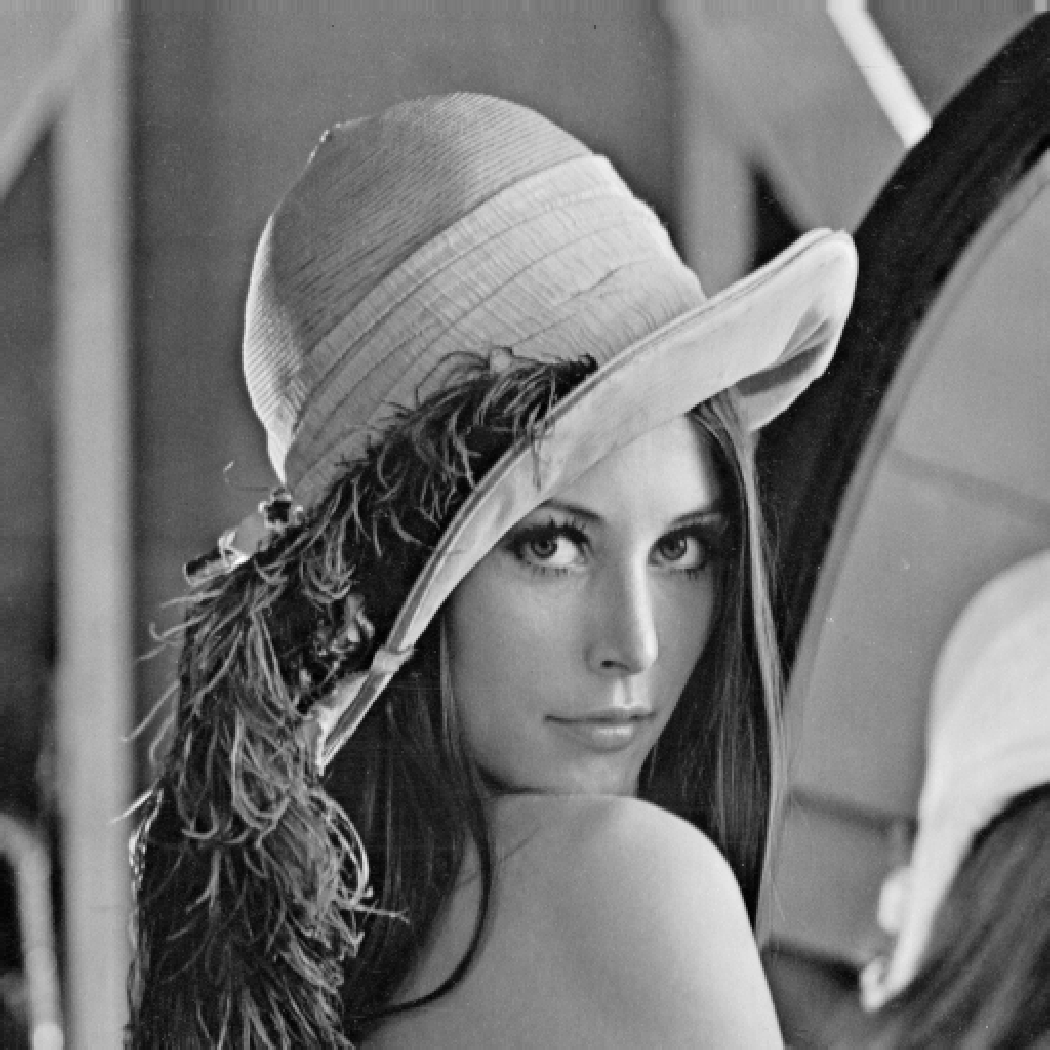
\includegraphics[width=0.32\textwidth]{../imagenes/LenaOriginal.pdf}}
  \subfloat[Pato]{
   \label{f:pato}
    
\includegraphics[width=0.32\textwidth]{../imagenes/duckOriginal.pdf}}
  \subfloat[Tigre]{
   \label{f:tigre}
    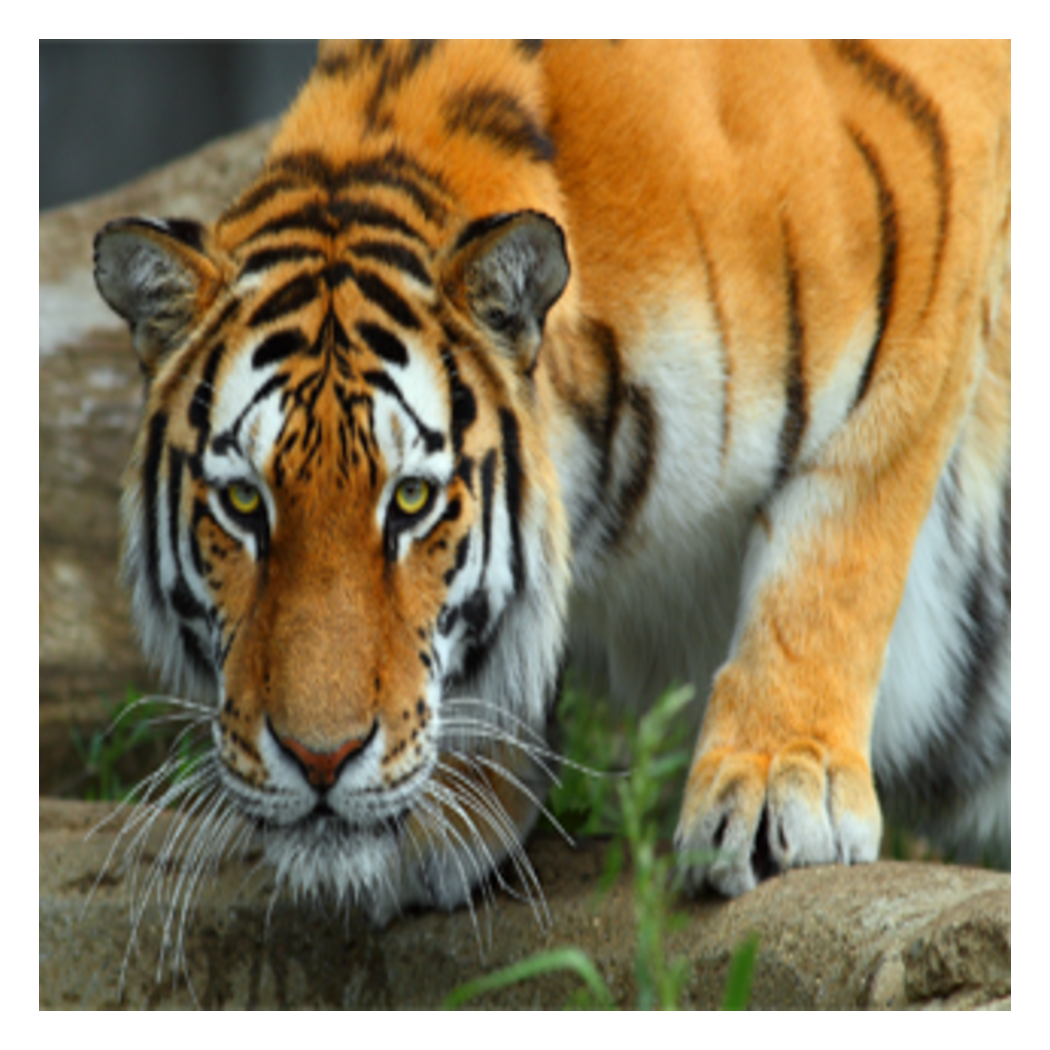
\includegraphics[width=0.34\textwidth]{../imagenes/tigerOriginal.pdf}}
 \caption{Imágenes utilizadas}
 \label{f:imgs}
\end{figure}

Se han elegido las tres imágenes anteriores por las siguientes razones:
\begin{enumerate}
\item Hay una en escala de grises y dos a color, por lo que se ha podido experimentar con imágenes a color, que presentan 3 matrices distintas, una para cada canal de color.
\item Hay una imagen más sencilla, la del pato, y dos con más detalles, para comprobar cómo se comporta el algoritmo en cada caso.
\item Hay dos imágenes más grandes (Lena es de 512x512 y la del pato de 500x546) y una más pequeña, la del tigre, que tiene 320x240.
\end{enumerate}

Intuitivamente, en el primer punto deberíamos obtener que la imagen reconstruida en escala de grises tiene más calidad que las imágenes en color, puesto que al reconstruir tres capas en lugar de una hay más posibilidad de perder información general a la hora de ver la imagen. Del mismo modo, en el segundo punto se debería obtener que la imagen más sencilla tiene más calidad que las otras dos, ya que debe ser más fácil reconstruir una serie prácticamente constante.\\ %En cuanto al tercer punto, parecería lógico pensar que cuanto más pequeña sea la imagen más fácil será de reconstruir, ya que \\

En un primer experimento, se han sacado las componentes principales con \texttt{k\_max = 5} y \texttt{expl\_var = 0.95} en los tres casos y se han reconstruido las imágenes con las componentes y los coeficientes obtenidos. En el caso de las imágenes a color se han separado los canales de color, sacado las componentes principales para cada canal, se ha reconstruido cada canal con sus componentes y se han vuelto a juntar para guardar la imagen. En el caso de la imagen de Lena, se han obtenido 12 componentes principales dinámicas. Para el pato se han obtenido 6, 5 y 6 para las capas R, G y B, respectivamente, y para el tigre 10, 13 y 11. Los resultados obtenidos han sido los mostrados en las figuras \ref{f:imgsLena}, \ref{f:imgsPato} y \ref{f:imgsTigre}.\\

Es conveniente notar que para poder mostrar las imágenes ha habido que reescalar los valores obtenidos por la reconstrucción de las series a los intervalos $[0,255]$ en el caso de imágenes en blanco y negro y a $[0,1]$ en cada capa en el caso de imágenes a color. Esto ha sido así por las dos funciones de \texttt{R} que se han utilizado para dibujar las imágenes, \texttt{image()} para el primer caso y \texttt{rasterImage()} para el segundo. En \texttt{image()} se umbralizan directamente los valores que superan el 255 o que están por debajo del 0, sin embargo \texttt{rasterImage()} no, por lo que se ha procedido a hacerlo manualmente. En este caso no se podía umbralizar porque las capas originales estaban en el intervalo $[0,255]$ por lo que se ha utilizado el homeomorfismo de cambio del intervalo $[\text{min},\text{max}]$ al intervalo $[0,1]$:
\[	x^{'} = \frac{x - \text{min}}{\text{max}-\text{min}} 	\]
con $x \in [\text{min},\text{max}]$.

\begin{figure}[H]
 \centering
  \subfloat[Imagen original]{
   \label{f:lenaO}
    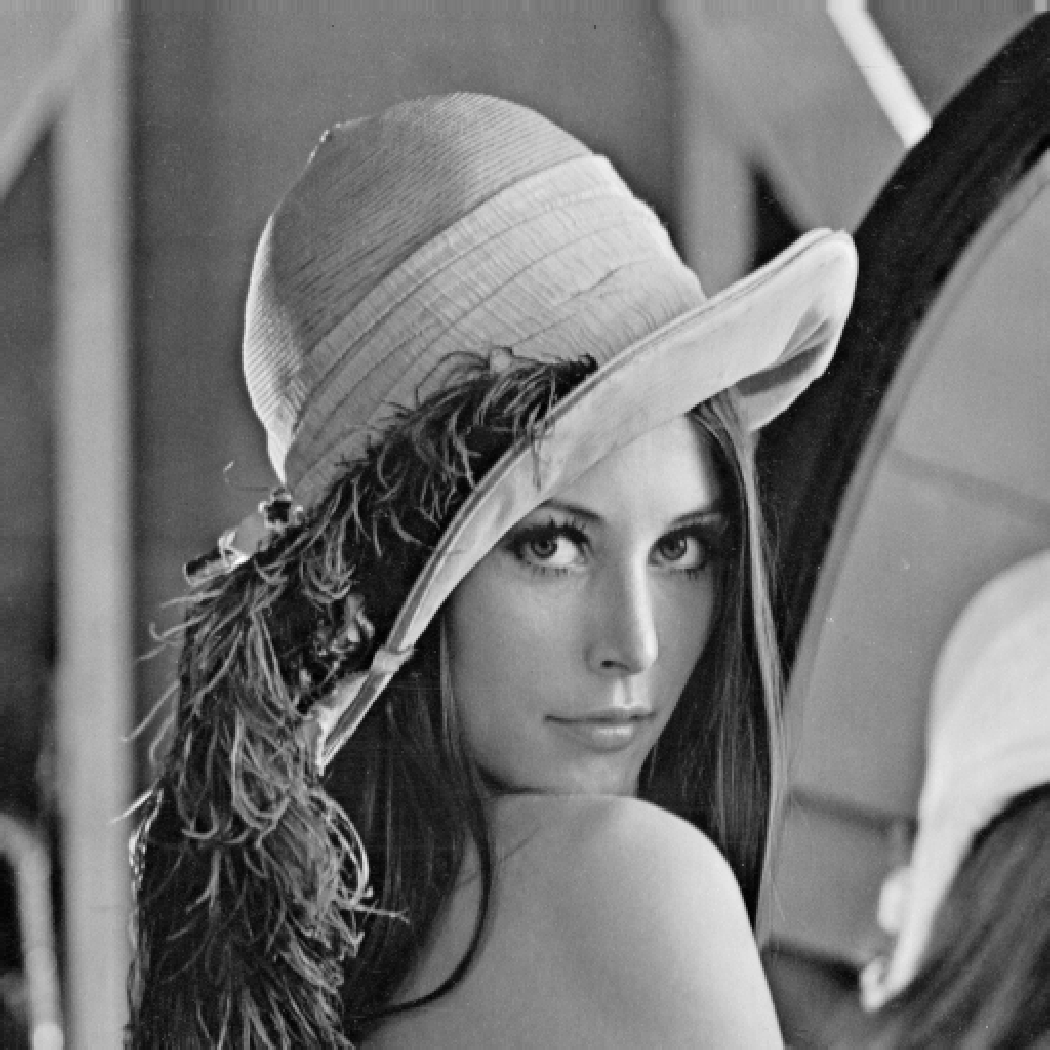
\includegraphics[width=0.5\textwidth]{../imagenes/LenaOriginal.pdf}}
  \subfloat[Imagen reconstruida]{
   \label{f:lenaR}
    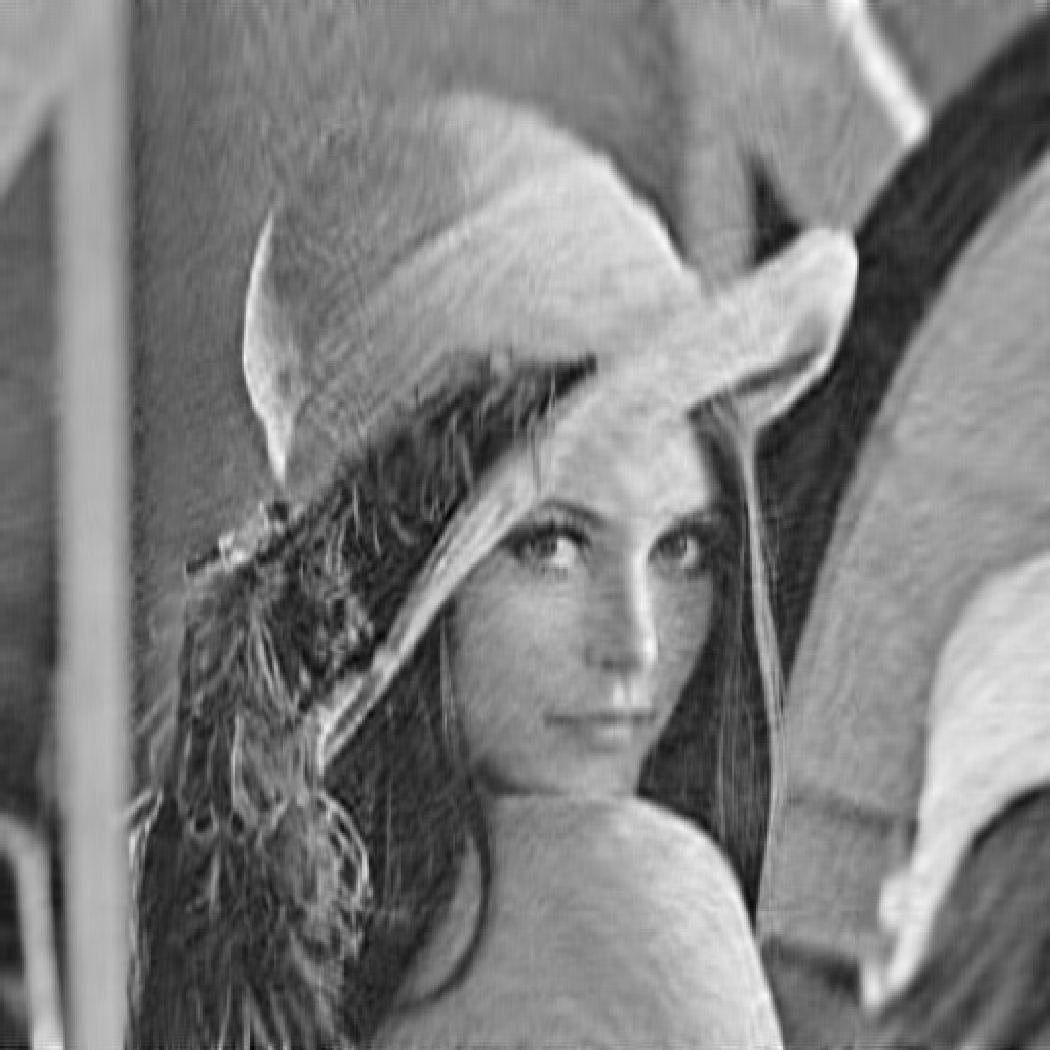
\includegraphics[width=0.5\textwidth]{../imagenes/lena095.pdf}}
 \caption{Lena}
 \label{f:imgsLena}
\end{figure}

\begin{figure}
 \centering
  \subfloat[Imagen original]{
   \label{f:patoO}
    
\includegraphics[width=0.5\textwidth]{../imagenes/duckOriginal.pdf}}
  \subfloat[Imagen reconstruida]{
   \label{f:patoR}
    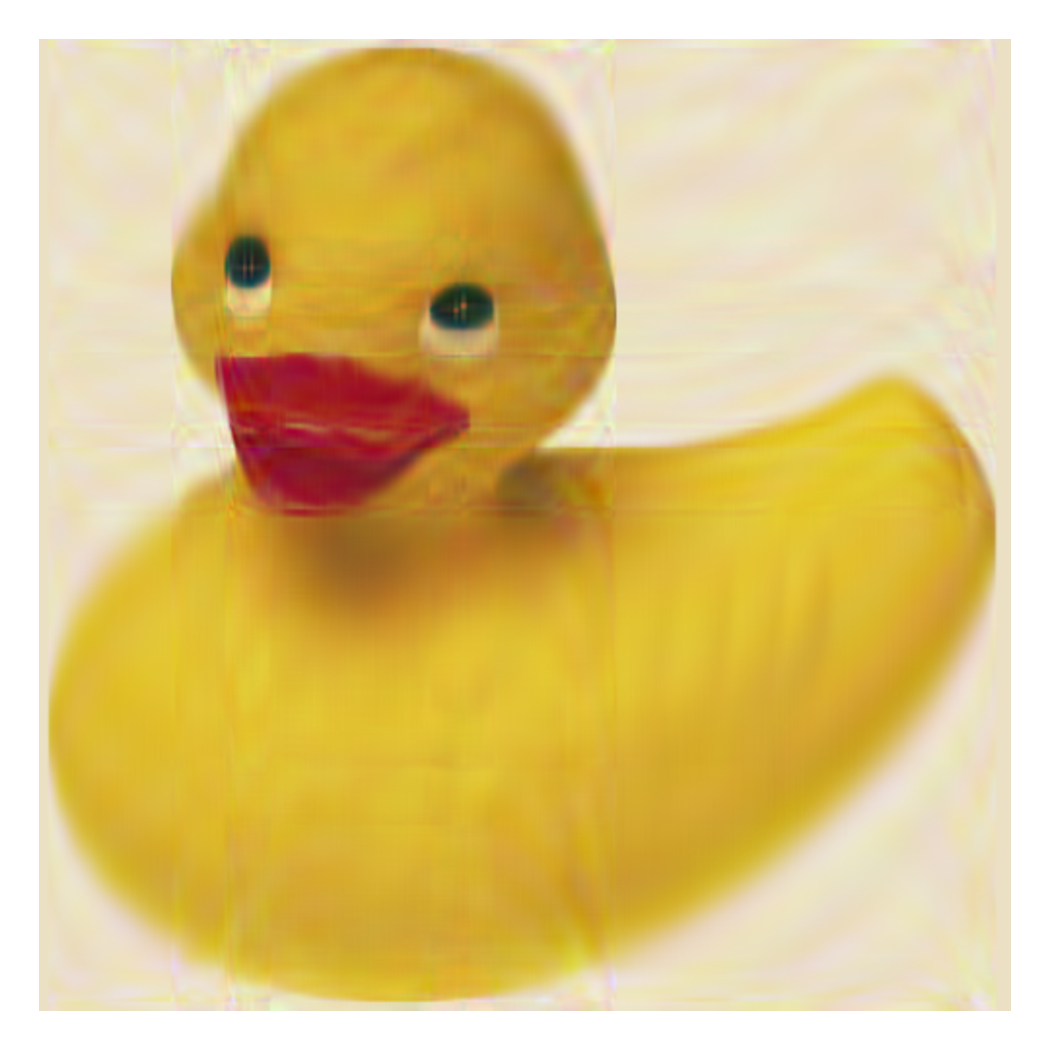
\includegraphics[width=0.5\textwidth]{../imagenes/duck095.pdf}}
 \caption{Pato}
 \label{f:imgsPato}
\end{figure}

\begin{figure}
 \centering
  \subfloat[Imagen original]{
   \label{f:tigreO}
    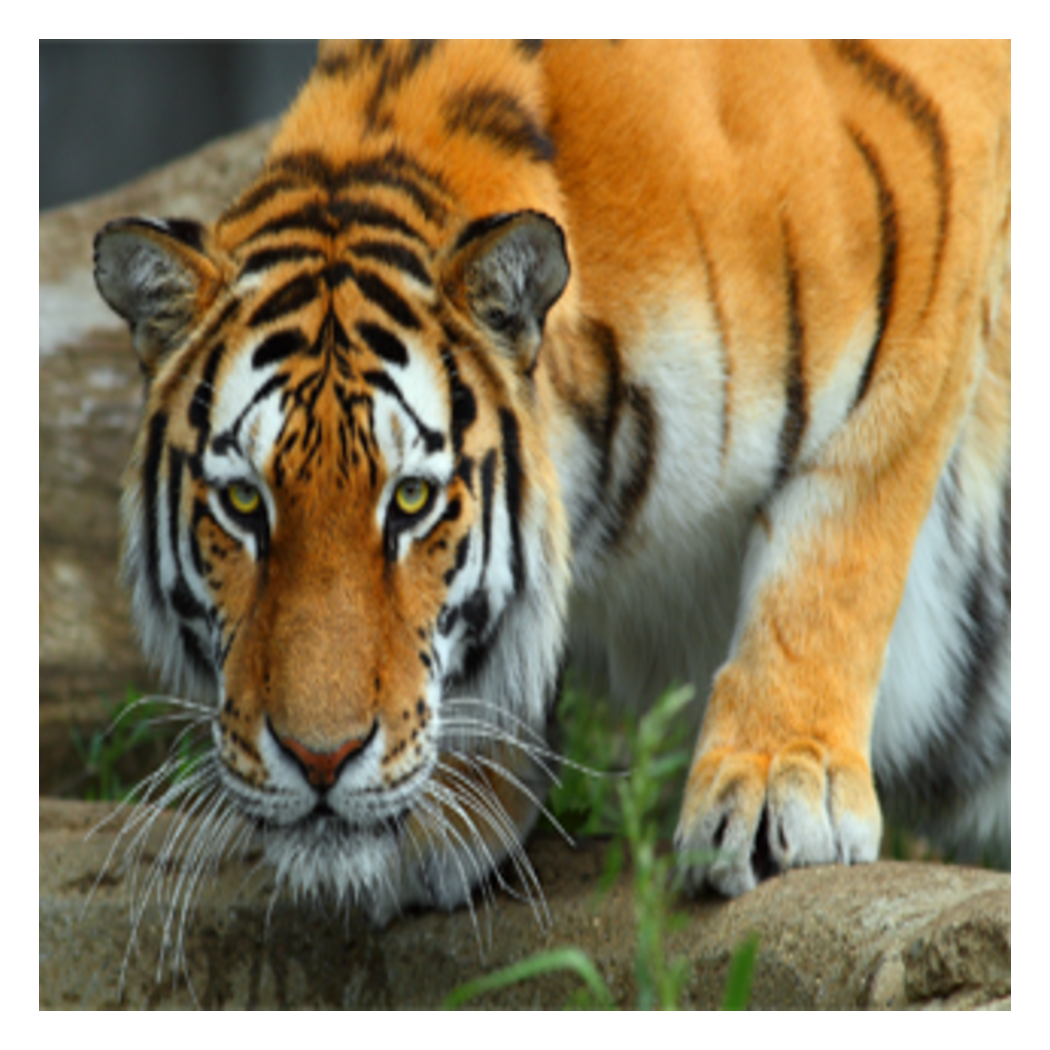
\includegraphics[width=0.5\textwidth]{../imagenes/tigerOriginal.pdf}}
  \subfloat[Imagen reconstruida]{
   \label{f:tigreR}
    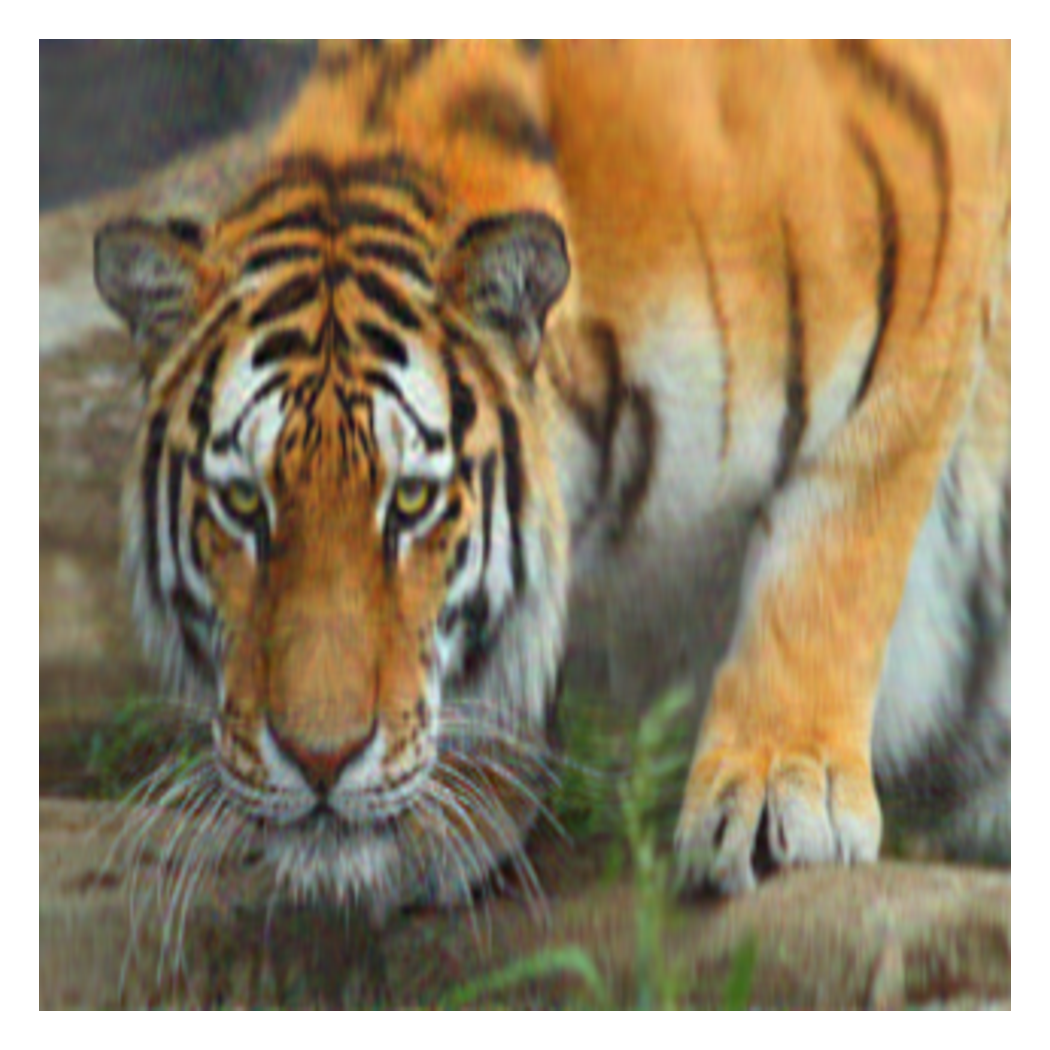
\includegraphics[width=0.5\textwidth]{../imagenes/tiger.pdf}}
 \caption{Tigre}
 \label{f:imgsTigre}
\end{figure}


Con estos experimentos podemos ver que en cuanto al segundo punto, las imágenes más simples no tienen por qué reconstruirse mejor, en contra de lo que se pensaba inicialmente, ya que la imagen más simple, que es la del pato, es la que peor se ve una vez se reconstruye. Esto es debido a que la mayor parte de las series en esa imagen (es decir, las columnas) son muy parecidas. De hecho, las componentes necesarias para explicar el 95\% de la varianza en esta imagen han sido menores que en las otras dos imágenes, concretamente la mitad de las componentes obtenidas con la imagen de Lena, que tiene casi la misma dimensión que la del pato, como se ha comentado antes. Esto implica que si los cambios en la imagen son pequeños (entendiendo como pequeños cambios suaves en el tono o color de la misma) normalmente se van a perder en la reconstrucción. Esto es lo que pasa por ejemplo con la parte del cuerpo del pato, donde está el detalle de las plumas. El cambio es demasiado suave entre todo el fondo amarillo y no es posible recogerlo en tan pocas componentes. Por esto, si los cambios son bruscos y las series difieren unas de otras harán falta más componentes para explicar el mismo porcentaje de varianza y por tanto el algoritmo tardará más pero también será mejor la reconstrucción. De esta forma, se explica que la imagen que peor se ve con respecto a la original sea la del pato, ya que tanto la de Lena como la del tigre tienen cambios más bruscos. De hecho, las partes de la imagen de Lena que son más uniformes en la imagen original se ven un poco peor en la imagen reconstruida.\\

Para ver esto más claro se ha cogido la imagen de Lena y se han hecho cambios en los niveles para pasar de una imagen prácticamente en negro a la imagen original. En este caso se ha hecho explicando el 90\% de varianza para reducir los tiempos de cómputo. Los resultados se pueden ver en las figuras \ref{f:imgsLenaN2}, \ref{f:imgsLenaN3}, \ref{f:imgsLenaN4}, \ref{f:imgsLenaN5} y \ref{f:imgsLenaN6}.\\

\begin{figure}
 \centering
  \subfloat[Imagen original]{
   \label{f:lenaN2O}
    
\includegraphics[width=0.5\textwidth]{../imagenes/nivelesLena2.pdf}}
  \subfloat[Imagen reconstruida]{
   \label{f:lenaN2R}
    
\includegraphics[width=0.5\textwidth]{../imagenes/nivelesLena2r.pdf}}
 \caption{Niveles de Lena}
 \label{f:imgsLenaN2}
\end{figure}

\begin{figure}
 \centering
  \subfloat[Imagen original]{
   \label{f:lenaN3O}
    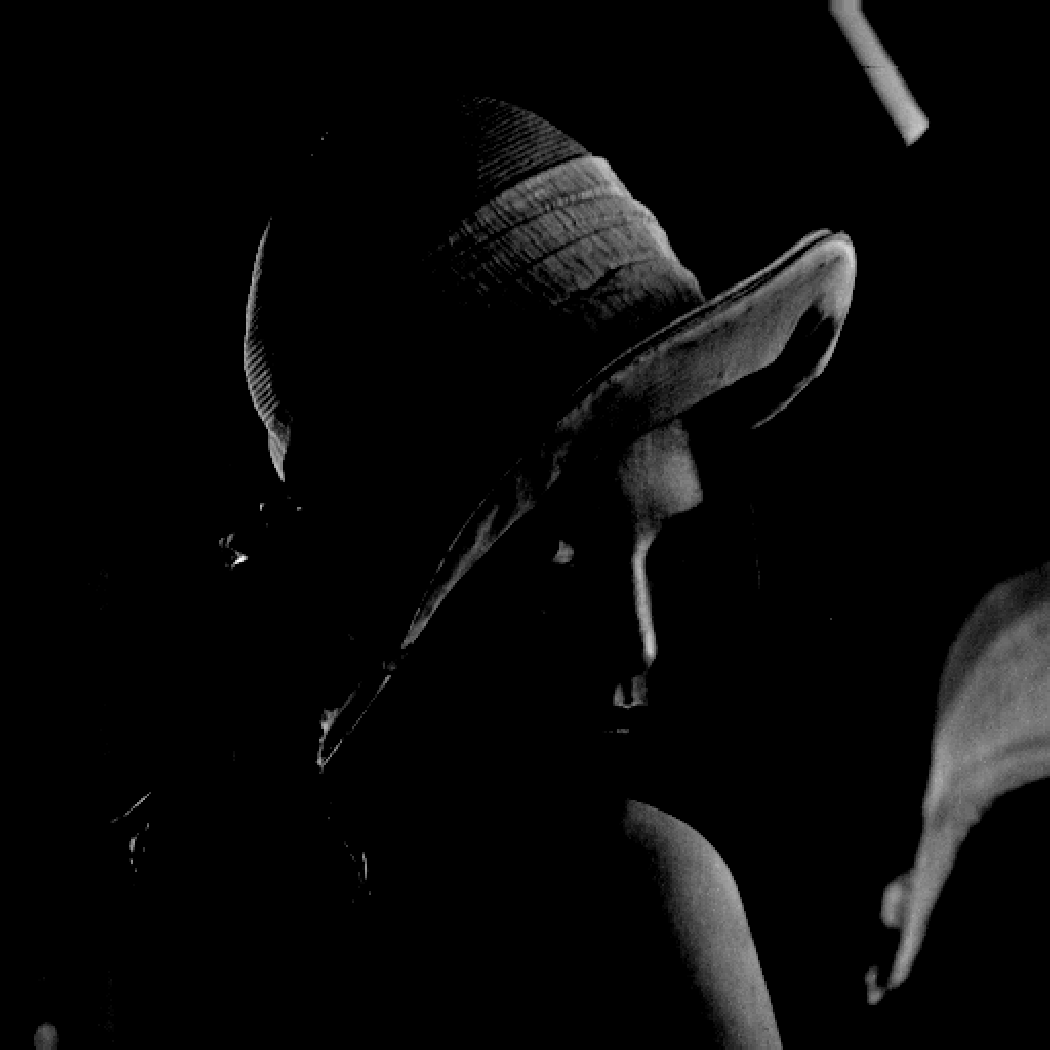
\includegraphics[width=0.5\textwidth]{../imagenes/nivelesLena3.pdf}}
  \subfloat[Imagen reconstruida]{
   \label{f:lenaN3R}
    
\includegraphics[width=0.5\textwidth]{../imagenes/nivelesLena3r.pdf}}
 \caption{Niveles de Lena}
 \label{f:imgsLenaN3}
\end{figure}

\begin{figure}
 \centering
  \subfloat[Imagen original]{
   \label{f:lenaN4O}
    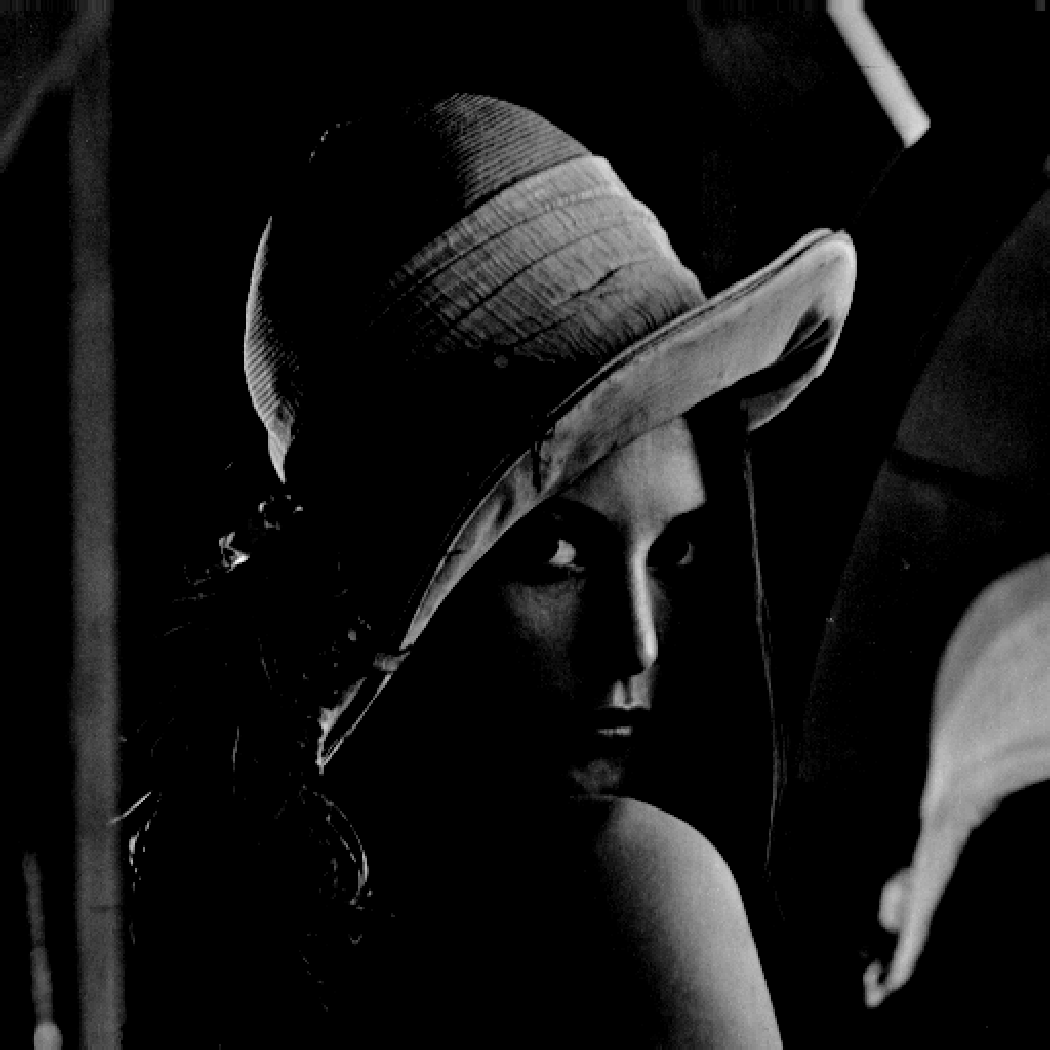
\includegraphics[width=0.5\textwidth]{../imagenes/nivelesLena4.pdf}}
  \subfloat[Imagen reconstruida]{
   \label{f:lenaN4R}
    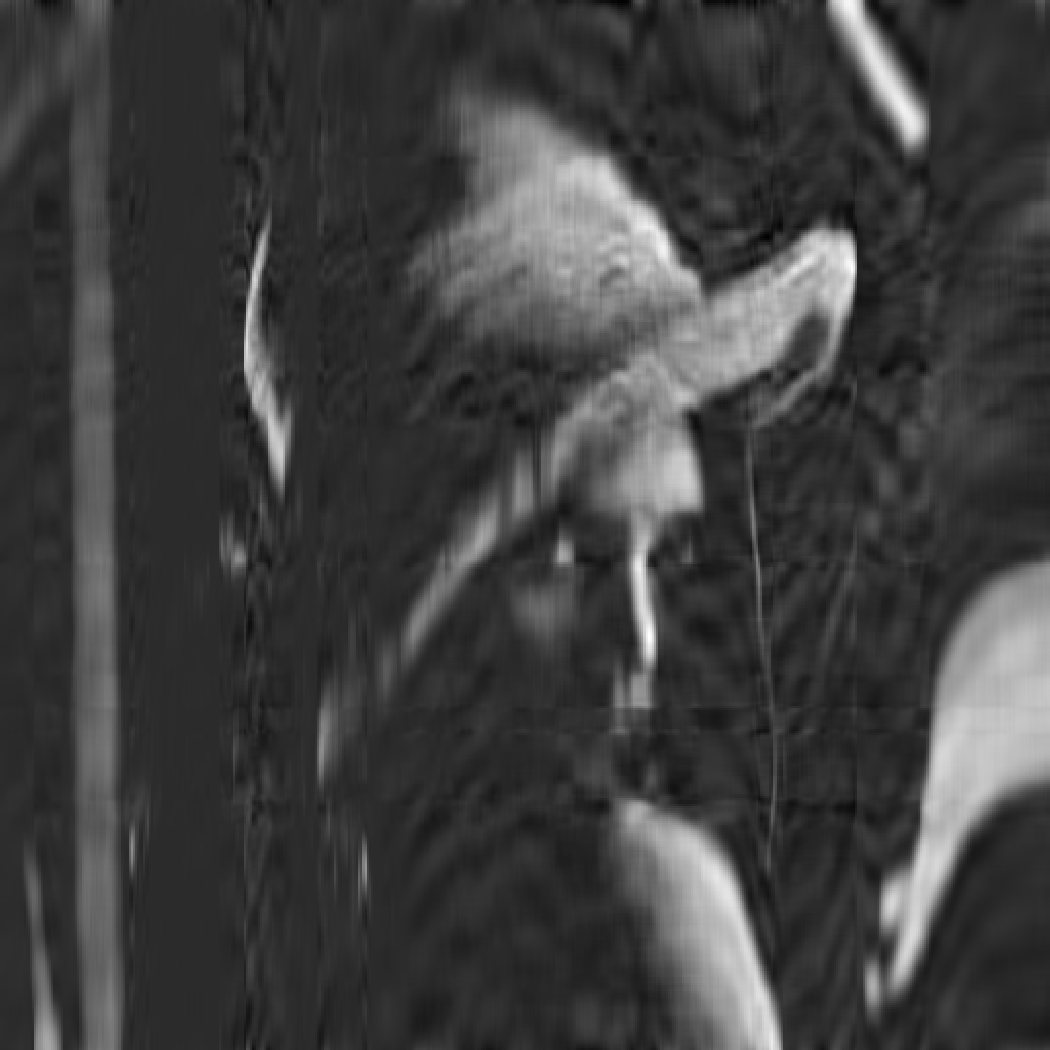
\includegraphics[width=0.5\textwidth]{../imagenes/nivelesLena4r.pdf}}
 \caption{Niveles de Lena}
 \label{f:imgsLenaN4}
\end{figure}

\begin{figure}
 \centering
  \subfloat[Imagen original]{
   \label{f:lenaN5O}
    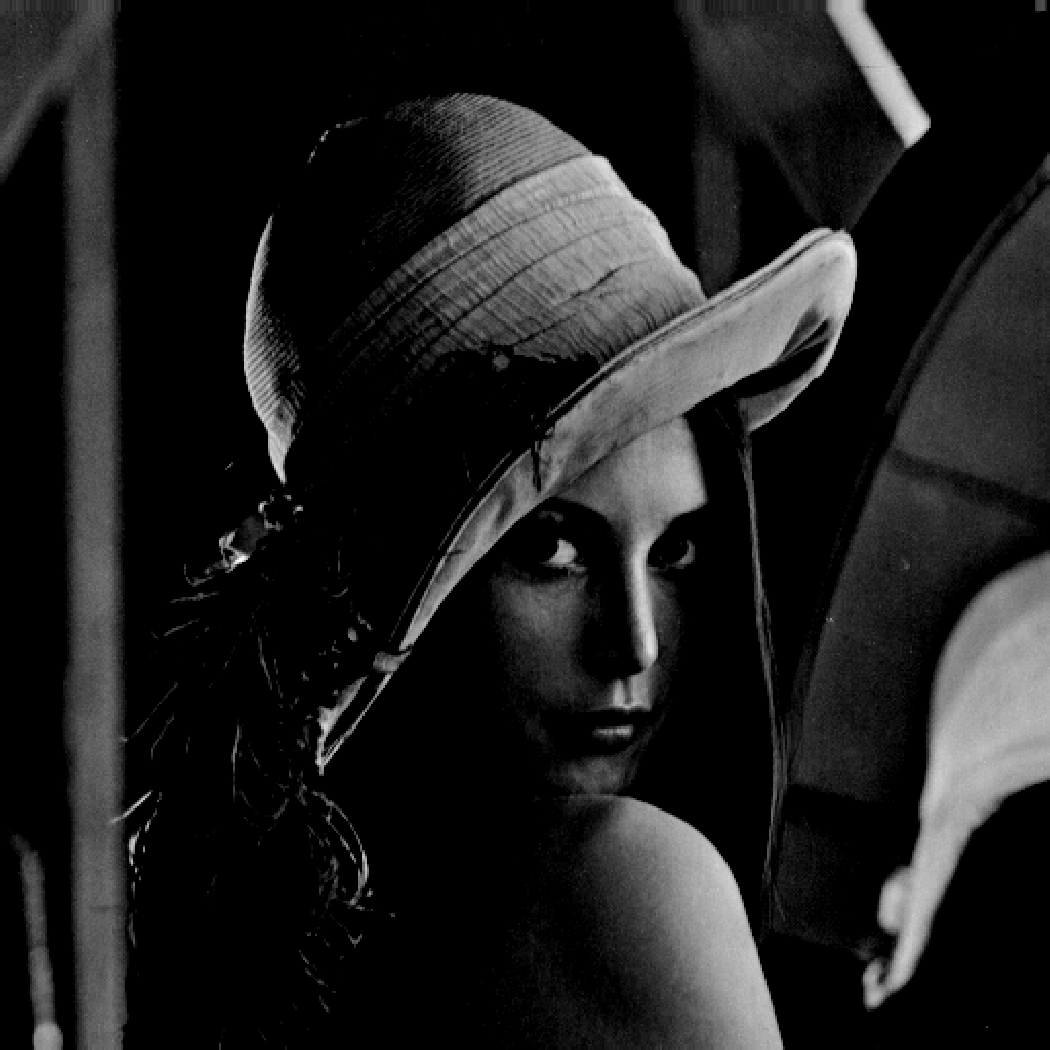
\includegraphics[width=0.5\textwidth]{../imagenes/nivelesLena5.pdf}}
  \subfloat[Imagen reconstruida]{
   \label{f:lenaN5R}
    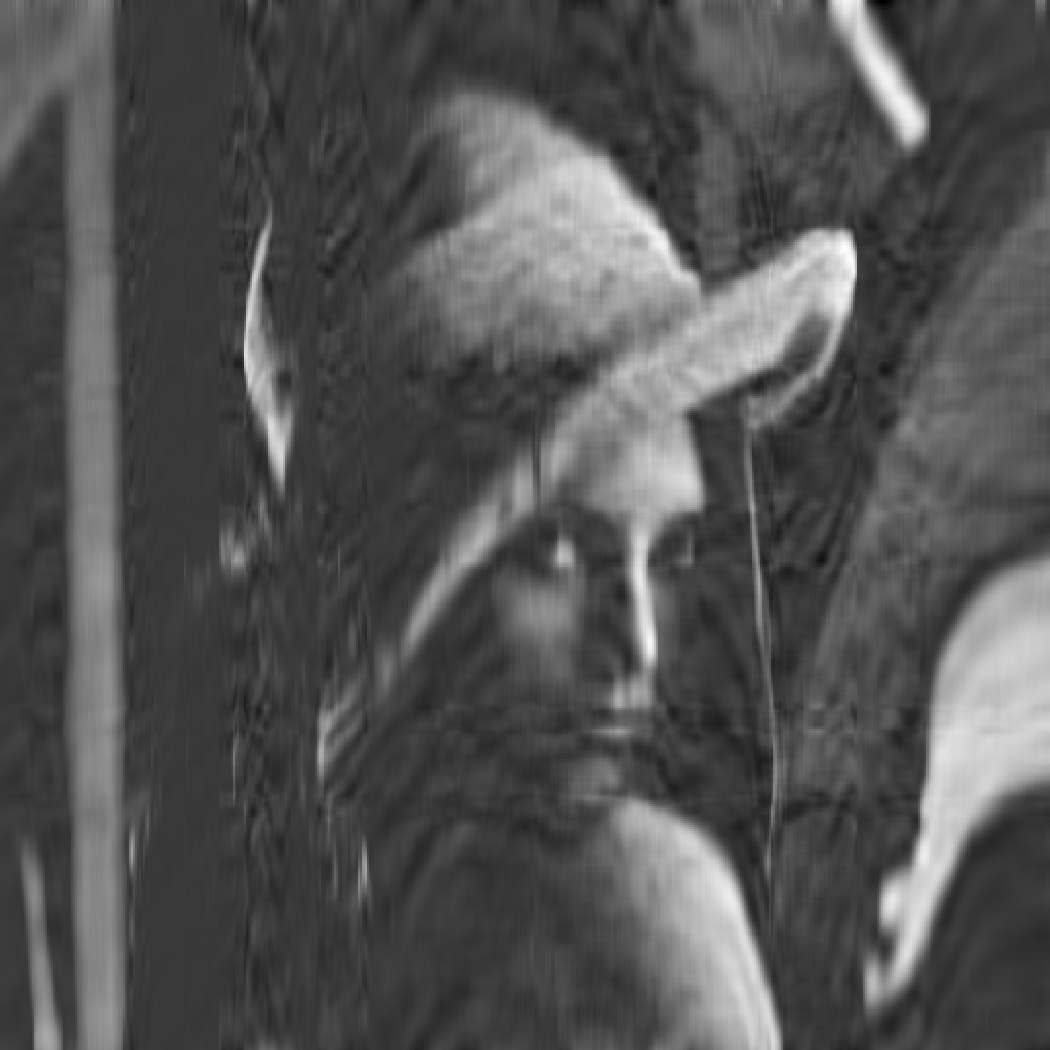
\includegraphics[width=0.5\textwidth]{../imagenes/nivelesLena5r.pdf}}
 \caption{Niveles de Lena}
 \label{f:imgsLenaN5}
\end{figure}

\begin{figure}
 \centering
  \subfloat[Imagen original]{
   \label{f:lenaN6O}
    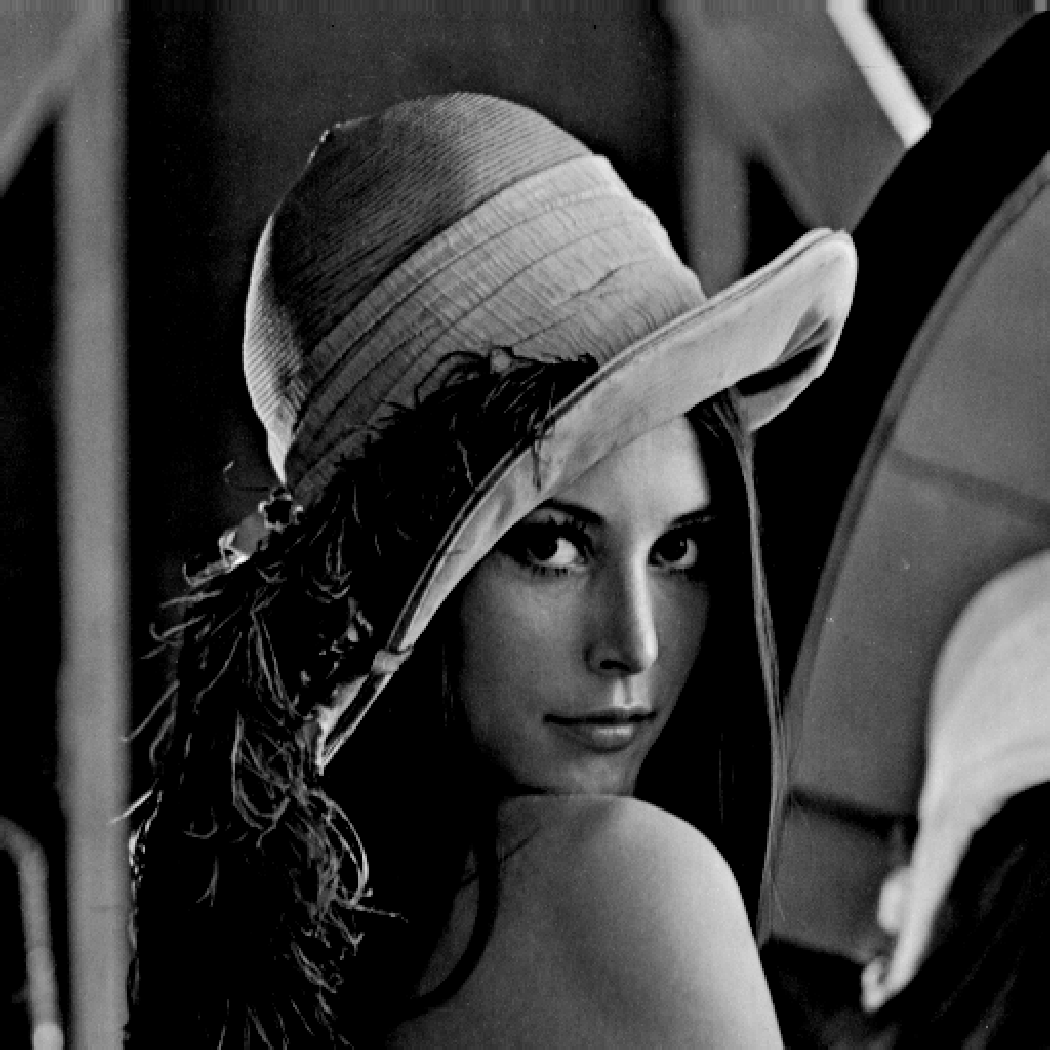
\includegraphics[width=0.5\textwidth]{../imagenes/nivelesLena6.pdf}}
  \subfloat[Imagen reconstruida]{
   \label{f:lenaN6R}
    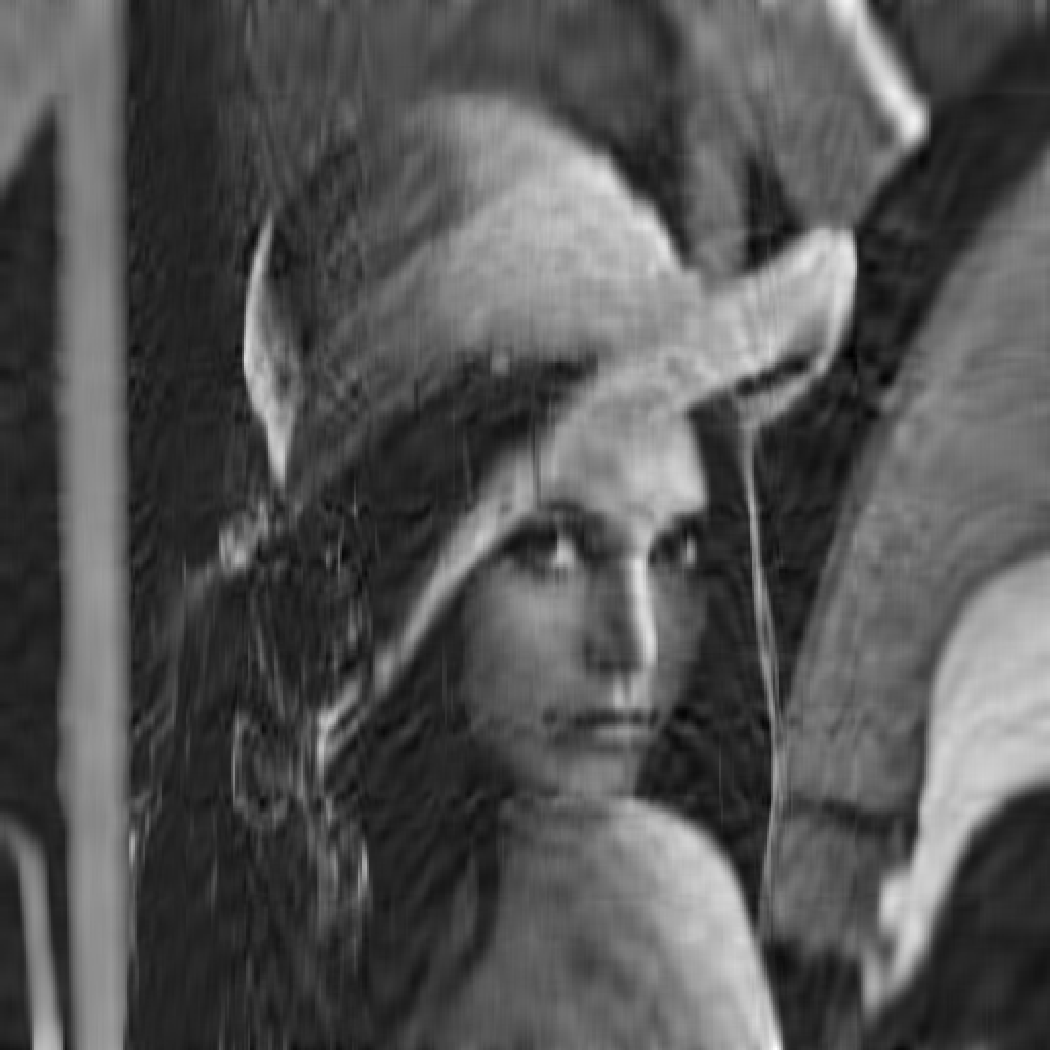
\includegraphics[width=0.5\textwidth]{../imagenes/nivelesLena6r.pdf}}
 \caption{Niveles de Lena}
 \label{f:imgsLenaN6}
\end{figure}

En la figura \ref{f:imgsLenaN2} podemos ver que si la imagen está prácticamente en el mismo color y lo único que aparece en ella tiene mucho contraste, es decir, los cambios en la serie son bruscos, entonces la reconstrucción es bastante buena. Sin embargo en las figuras de la \ref{f:imgsLenaN3} a la \ref{f:imgsLenaN5} vamos viendo como según los cambios son menos bruscos y hay suficiente negro en la imagen, se van viendo peor las reconstrucciones para de nuevo, como podemos ver en la figura \ref{f:imgsLenaN6} y en la original, según van desapareciendo las partes constantes en negro y apareciendo los detalles en distintos tonos (es decir, las series dejan de ser constantes y parecidas) irse viendo con más calidad la imagen reconstruida.\\

Hay que tener en cuenta que para estas reconstrucciones se han sacado componentes principales hasta explicar (como mínimo) el 90\% de varianza y no el 95\%, como estaban hechas las imágenes anteriores. La diferencia entre reconstruir la imagen de Lena original con el 90\% y el 95\% está en la figura \ref{f:imgsLena09}. Es por esto que tampoco se ven con tanta calidad como la imagen reconstruida en la figura \ref{f:lena095}.\\

\begin{figure}
 \centering
  \subfloat[Imagen al 90\%]{
   \label{f:lena090}
    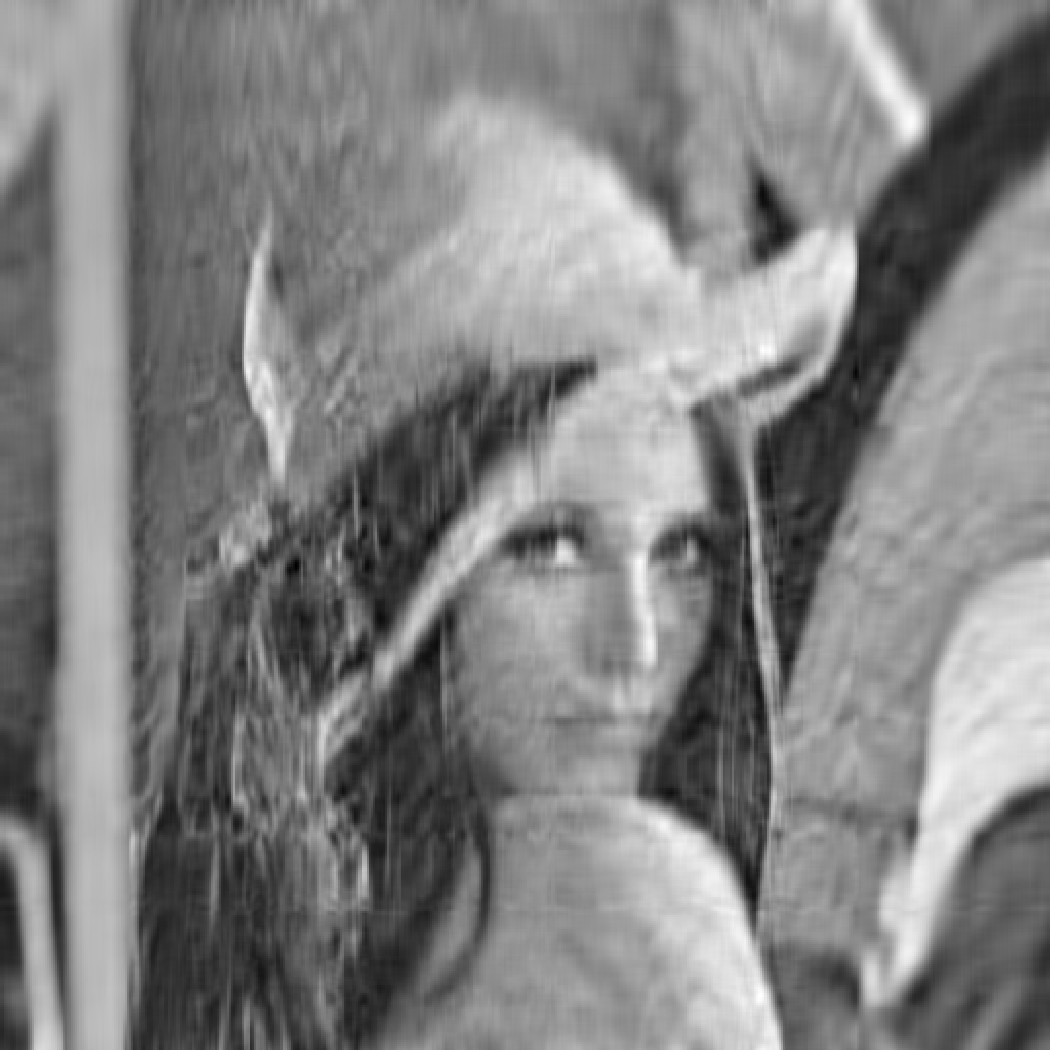
\includegraphics[width=0.5\textwidth]{../imagenes/lena090.pdf}}
  \subfloat[Imagen al 95\%]{
   \label{f:lena095}
    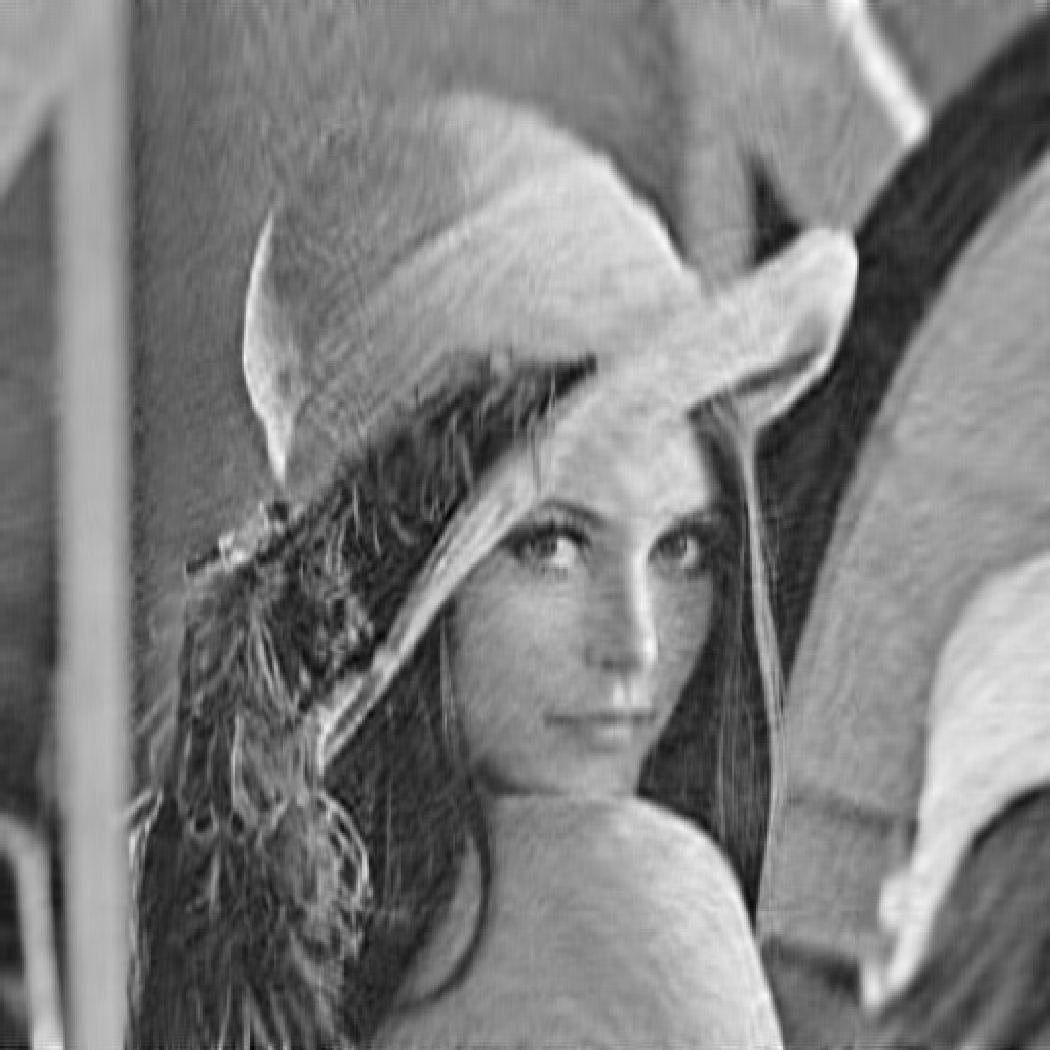
\includegraphics[width=0.5\textwidth]{../imagenes/lena095.pdf}}
 \caption{Reconstrucciones de Lena}
 \label{f:imgsLena09}
\end{figure}

Vamos a ver ahora el factor de compresión que se consigue con cada una de las tres imágenes que hemos utilizado sacando las componentes explicando como mínimo un 95\% de varianza. Esto se puede ver en el cuadro \ref{t:compresion}, donde los cálculos se han hecho de la siguiente forma:
\begin{itemize}
\item El factor de compresión se medirá dividiendo el número de números que son necesarios para almacenar la imagen original entre el número de números necesarios para almacenar lo necesario para reconstruir la imagen, suponiendo que todos los números se almacenan con la misma precisión.
\item En el caso de la imagen original se necesitarán $\text{nº de filas}\times \text{nº de columnas} \times \text{nº de canales}$, ya que se almacena una matriz de píxeles de esas dimensiones.
\item En el caso de las reconstruidas, se almacenan $n$ componentes principales dinámicas y para cada componente principal dinámica de tamaño $T+k$ con $T$ el número de valores en cada serie (el número de filas en este caso) y $k$ el número de lags utilizados en esa componente, se almacena también una matriz de coeficientes $\beta$ de tamaño $m\times (k+1)$, con $m$ el número de series (el número de columnas en este caso) y un vector de coeficientes $\alpha$ de tamaño $m$, por lo que para cada componente se utilizan $(T+k)+m \times (k+1) + m$ y el número total será la suma de estos números para cada componente.
\end{itemize}

\begin{table}[]
\centering
\caption{Factor de compresión}
\label{t:compresion}
\resizebox{\textwidth}{!}{\begin{tabular}{|cc|c|c|c|c|c|c|c|c|}
\hline
                            &         & T   & m   & \begin{tabular}[c]{@{}c@{}}nº\\ componentes\end{tabular} & \begin{tabular}[c]{@{}c@{}}k utilizados\\ (por orden)\end{tabular}                  & nº a almacenar & \begin{tabular}[c]{@{}c@{}}Total en\\ reconstruida\end{tabular} & \begin{tabular}[c]{@{}c@{}}Total en \\ original\end{tabular} & \begin{tabular}[c]{@{}c@{}}Factor de \\ compresión\end{tabular} \\ \hline
Lena                        &         & 512 & 512 & 12                                                       & \begin{tabular}[c]{@{}c@{}}5, 3, 5, 4, 5, 4, \\ 5, 4, 5, 5, 5, 5\end{tabular}       & 46647          & 46647                                                           & 262144                                                       & 5,61974                                                         \\ \hline
\multicolumn{1}{|c|}{}      & Canal R & 546 & 500 & 6                                                        & 4, 4, 5, 4, 5, 5                                                                    & 22803          &                                                                 &                                                              &                                                                 \\ \cline{2-7}
\multicolumn{1}{|c|}{Pato}  & Canal G & 546 & 500 & 5                                                        & 3, 4, 5, 5, 5                                                                       & 18752          & 62855                                                           & 819000                                                       & 13,02999                                                        \\ \cline{2-7}
\multicolumn{1}{|c|}{}      & Canal B & 546 & 500 & 6                                                        & 2, 4, 4, 4, 5, 5                                                                    & 21300          &                                                                 &                                                              &                                                                 \\ \hline
\multicolumn{1}{|c|}{}      & Canal R & 240 & 320 & 10                                                       & \begin{tabular}[c]{@{}c@{}}4, 5, 5, 5, 5, \\ 5, 5, 5, 5, 5\end{tabular}             & 24529          &                                                                 &                                                              &                                                                 \\ \cline{2-7}
\multicolumn{1}{|c|}{Tigre} & Canal G & 240 & 320 & 13                                                       & \begin{tabular}[c]{@{}c@{}}5, 5, 5, 5, 5, \\ 5, 5, 5, 5, 5, \\ 4, 5, 4\end{tabular} & 31663          & 82885                                                           & 230400                                                       & 2,779755                                                        \\ \cline{2-7}
\multicolumn{1}{|c|}{}      & Canal B & 240 & 320 & 11                                                       & \begin{tabular}[c]{@{}c@{}}4, 5, 5, 5, 5, \\ 5, 4, 5, 5, 5, 5\end{tabular}          & 26693          &                                                                 &                                                              &                                                                 \\ \hline
\end{tabular}}
\end{table}

Como vemos en dicha tabla, el factor de compresión depende de cómo de simple sea la imagen, de forma que tenemos que la más simple consigue un factor de compresión de más de 13 y la que tiene más detalles un factor de compresión de casi 3, mientras que Lena, que también tiene bastantes detalles, tiene un factor de compresión de más de 5. Teniendo en cuenta que las componentes principales dinámicas para estas imágenes se han generado exigiendo que se explicara un 95\% de varianza como mínimo, estos factores de compresión son bastante altos, ya que como muy poco se guarda menos de la mitad de la información original.\\


Cabe ahora preguntarse si habría alguna diferencia significativa entre utilizar como series temporales las columnas de la imagen como hemos estado haciendo hasta ahora o utilizar las filas. La intuición nos dice que no debe haber mucha diferencia por lo comentado anteriormente: si un pixel se parece a los que tiene alrededor, tanto las columnas cercanas van a parecerse como series como las filas. Se ha hecho una prueba con la imagen de Lena reconstruida por filas y por columnas y la comparación puede verse en la figura \ref{f:comparativaFilas}.\\

\begin{figure}
 \centering
  \subfloat[Imagen reconstruida por columnas]{
   \label{f:lena095C}
    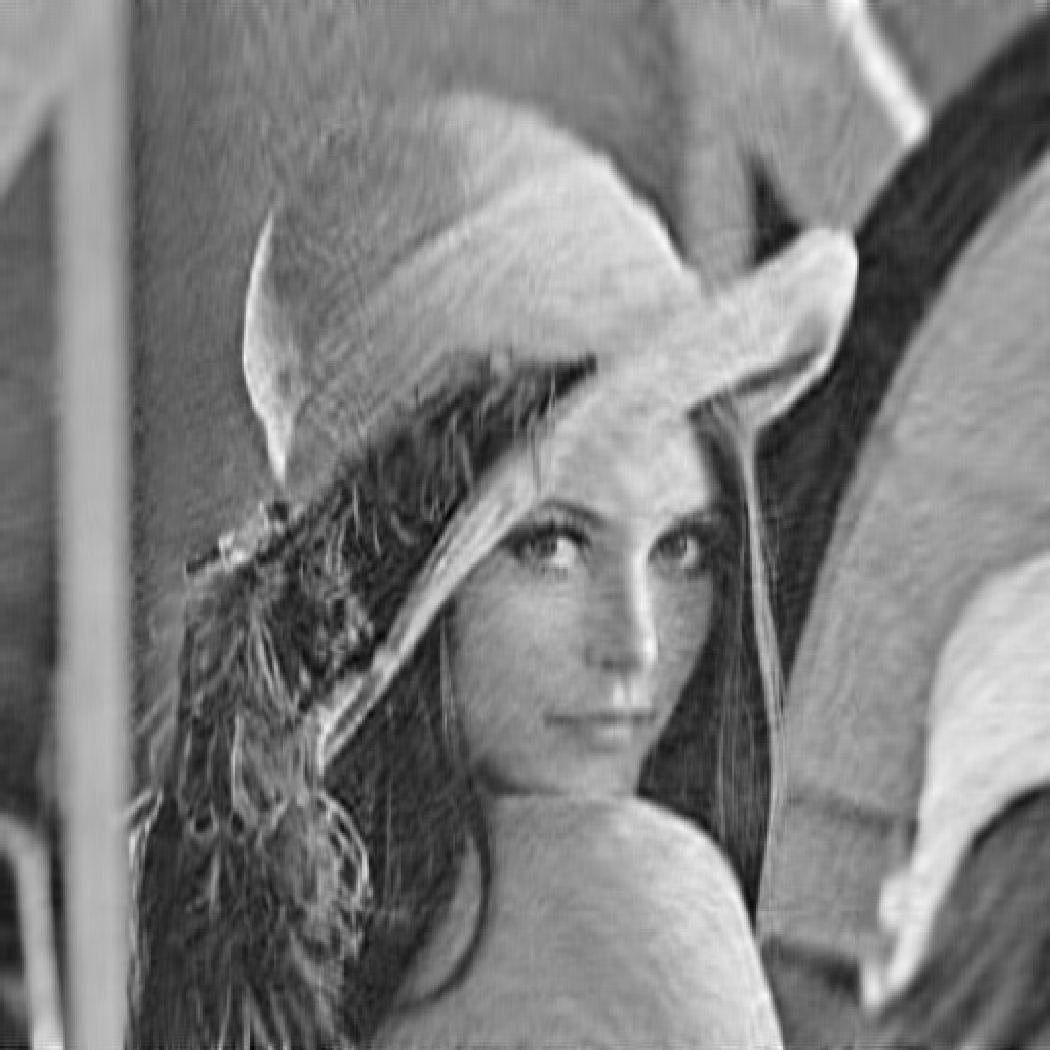
\includegraphics[width=0.5\textwidth]{../imagenes/lena095.pdf}}
  \subfloat[Imagen reconstruida por filas]{
   \label{f:lena095}
    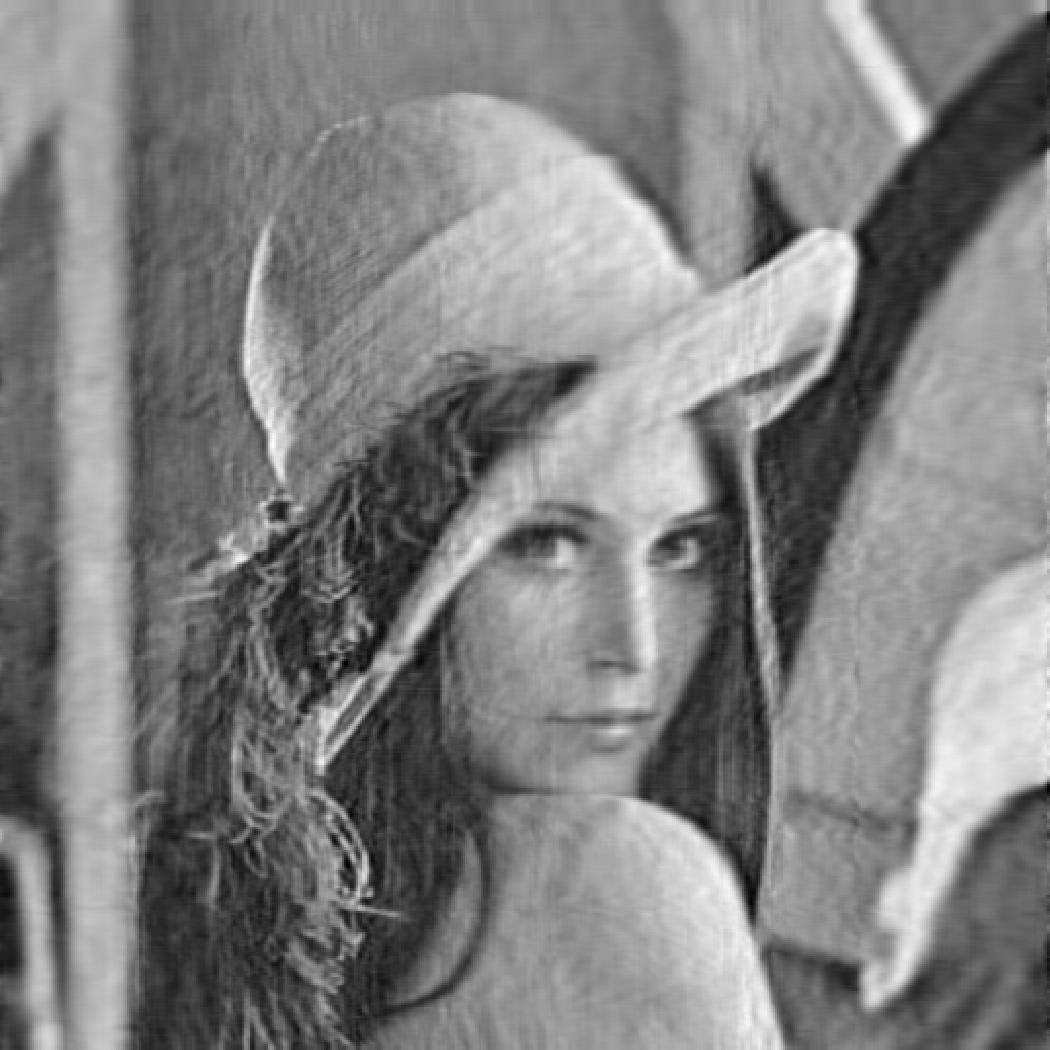
\includegraphics[width=0.5\textwidth]{../imagenes/lenaFilas095.pdf}}
 \caption{Reconstrucciones de Lena}
 \label{f:comparativaFilas}
\end{figure}

Efectivamente, las diferencias no son significativas. Sí que podemos observar que hay partes más nítidas en una que en otra. Por ejemplo, los ojos están más nítidos en la imagen reconstruida por columnas y la parte superior del sombrero está más nítida en la imagen reconstruida por filas.\\

Como último experimento dentro de la compresión de imágenes se ha elegido ver las reconstrucciones con sucesivas componentes principales dinámicas, acumulándolas, para ver el efecto que éstas tienen en la reconstrucción de las series originales. Es decir, hemos cogido la imagen de Lena y la hemos reconstruido sólo con la primera componente, después con la primera y la segunda, etcétera, hasta llegar a las 12 componentes que obtiene el método \texttt{auto.gdpc}. El resultado de estos experimentos se puede ver en las figuras \ref{f:RLenaC1}, \ref{f:RLenaC2}, \ref{f:RLenaC3} y \ref{f:RLenaC4}.

\begin{figure}[]
 \centering
  \subfloat[Componente 1]{
   \label{f:lena0951}
    \includegraphics[width=0.33\textwidth]{../imagenes/lena0951.pdf}}
  \subfloat[Componentes 1 y 2]{
   \label{f:lena0952}
    \includegraphics[width=0.33\textwidth]{../imagenes/lena0952.pdf}}
  \subfloat[Componentes 1, 2 y 3]{
   \label{f:lena0953}
    \includegraphics[width=0.33\textwidth]{../imagenes/lena0953.pdf}}
 \caption{Reconstrucciones de Lena con distintas componentes}
 \label{f:RLenaC1}
\end{figure}

\begin{figure}[]
 \centering
  \subfloat[Componentes 1 a 4]{
   \label{f:lena0954}
    \includegraphics[width=0.33\textwidth]{../imagenes/lena0954.pdf}}
  \subfloat[Componentes 1 a 5]{
   \label{f:lena0955}
    \includegraphics[width=0.33\textwidth]{../imagenes/lena0955.pdf}}
  \subfloat[Componentes 1 a 6]{
   \label{f:lena0956}
    \includegraphics[width=0.33\textwidth]{../imagenes/lena0956.pdf}}
 \caption{Reconstrucciones de Lena con distintas componentes}
 \label{f:RLenaC2}
\end{figure}


\begin{figure}[]
 \centering
  \subfloat[Componentes 1 a 7]{
   \label{f:lena0957}
    \includegraphics[width=0.33\textwidth]{../imagenes/lena0957.pdf}}
  \subfloat[Componentes 1 a 8]{
   \label{f:lena0958}
    \includegraphics[width=0.33\textwidth]{../imagenes/lena0958.pdf}}
  \subfloat[Componentes 1 a 9]{
   \label{f:lena0959}
    \includegraphics[width=0.33\textwidth]{../imagenes/lena0959.pdf}}
 \caption{Reconstrucciones de Lena con distintas componentes}
 \label{f:RLenaC3}
\end{figure}

\begin{figure}[]
 \centering
  \subfloat[Componentes 1 a 10]{
   \label{f:lena09510}
    \includegraphics[width=0.33\textwidth]{../imagenes/lena09510.pdf}}
  \subfloat[Componentes 1 a 11]{
   \label{f:lena09511}
    \includegraphics[width=0.33\textwidth]{../imagenes/lena09511.pdf}}
  \subfloat[Componentes 1 a 12]{
   \label{f:lena09512}
    \includegraphics[width=0.33\textwidth]{../imagenes/lena09512.pdf}}
 \caption{Reconstrucciones de Lena con distintas componentes}
 \label{f:RLenaC4}
\end{figure}

Como se puede observar, la mejora de la reconstrucción conforme se van agregando componentes hasta la octava es obvia, ya que se pasa de ver una simple silueta a ver la imagen original. Agregar la información que aportan el resto de componentes le da a la reconstrucción la nitidez que veíamos al principio. Esto es así porque la información que va aportando cada componente se suma a la que información de la que ya se disponía, como se ha comentado antes.\\ %TODO

%TODO conclusiones en la utilización a compresión de imágenes en general

\section{Aplicación: Búsqueda de patrones en series periódicas}

Una de las técnicas en el preprocesamiento de series es eliminar los periodos de las series originales, ya que es uno de los pasos para hacerlas estacionarias, en caso de que éstas sean periódicas. Se ha pensado en utilizar el algoritmo GDPC para obtener el patrón periódico de la serie y restárselo directamente a la serie original por periodos. Para ello, se toma la serie original y se divide en periodos y se coloca cada trozo de la serie original como una columna de una matriz, sobre la que se pasará el GDPC. Al ser las series parecidas, lo más probable es que sólo se obtenga una componente principal dinámica, de modo que ésta será la que utilicemos. En caso de que se obtenga más de una, siempre se puede aumentar \texttt{k\_max} o disminuir un poco \texttt{expl\_var} en el algoritmo para obtener una sola componente principal dinámica.\\

Para probar si de hecho se pueden utilizar las componentes principales dinámicas para la detección de patrones o no, se ha hecho un experimento con una serie real que tiene una tendencia periódica. Esta serie es la cantidad de accidentes de coche mensuales en Italia desde enero de 1983 hasta diciembre de 1997, obtenida de la referencia %TODO
y que se puede ver en la figura \ref{f:accidents}. Como se puede ver esta serie presenta una clara tendencia periódica, lo que tiene sentido porque hay más accidentes en verano que en invierno.

\begin{figure}[]
 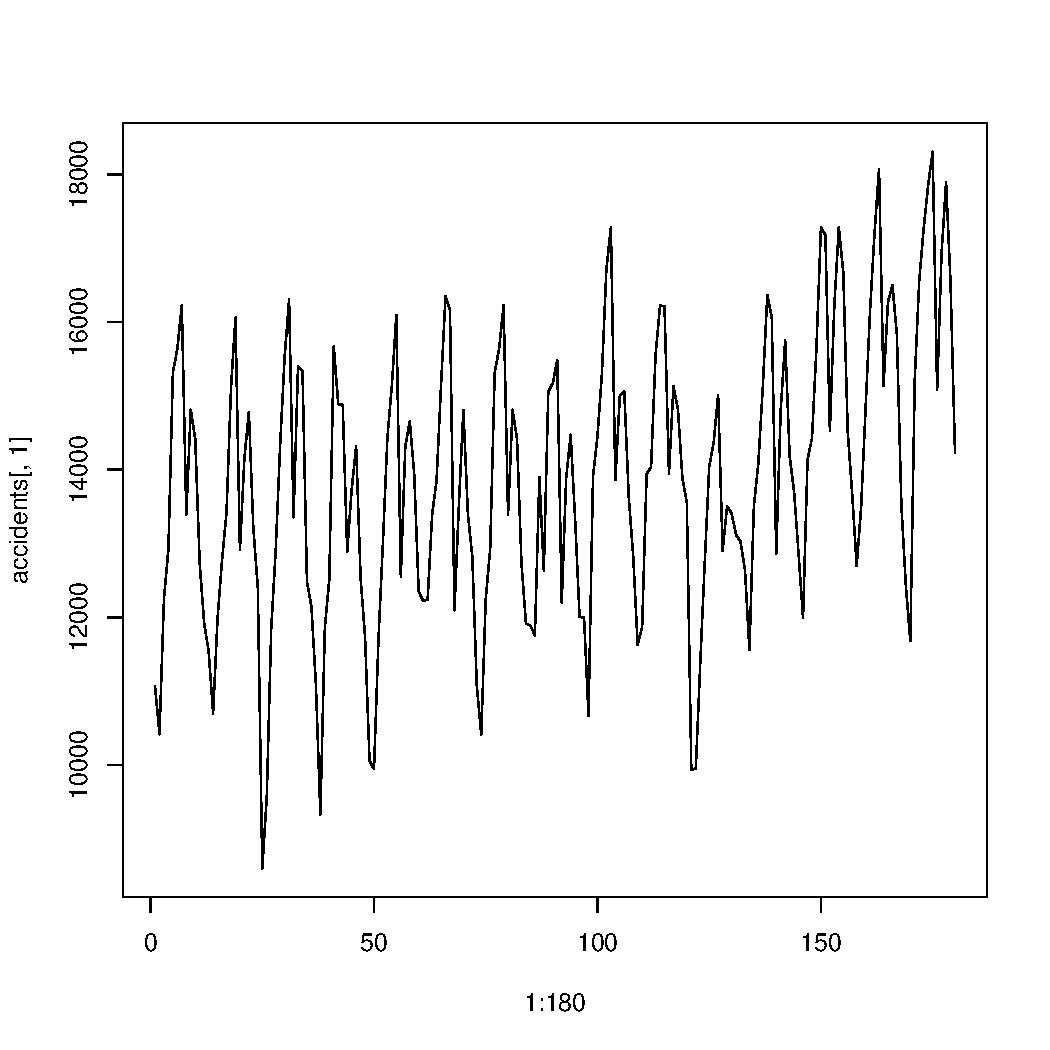
\includegraphics[width=\textwidth, height=0.4\textheight]{../imagenes/accidents.pdf}
 \caption{Número mensual de accidentes de coche en Italia de 1983 a 1997}
 \label{f:accidents}
\end{figure}

Lo que hacemos ahora es cortar trozos de esta serie de la forma en la que aparece en la figura \ref{f:periodos} de forma que cada serie consta de 13 puntos, y los metemos todos en una matriz, por columnas, para obtener la primera componente principal. En este caso se consigue sólo una imponiendo en el algoritmo \texttt{k\_max=5} y \texttt{expl\_var=0.95}. El resultado de esta componente está en la figura \ref{f:accidentsComp}.

\begin{figure}[]
 \centering
  \subfloat[Primer periodo]{
   \label{f:periodo1}
    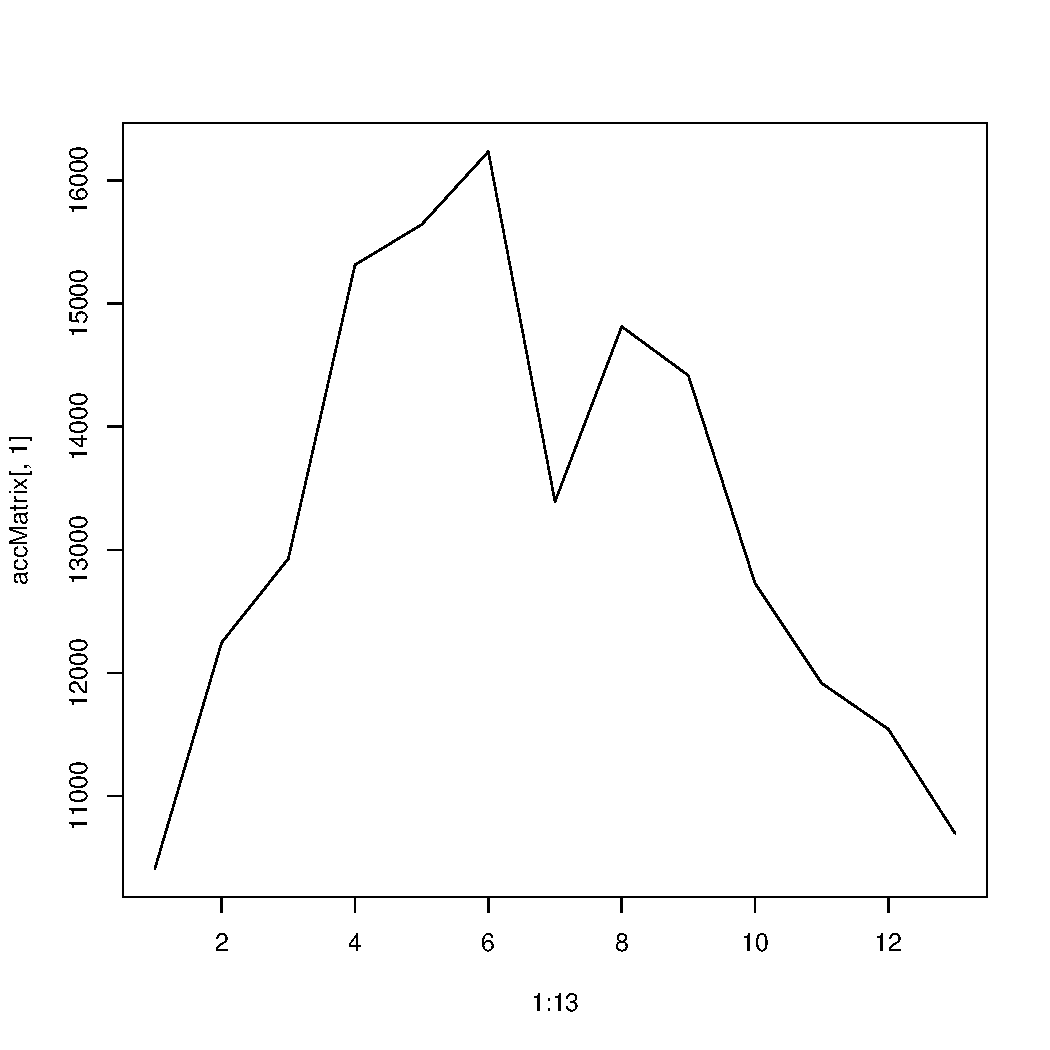
\includegraphics[width=0.33\textwidth]{../imagenes/primerPeriodo.pdf}}
  \subfloat[Segundo periodo]{
   \label{f:periodo2}
    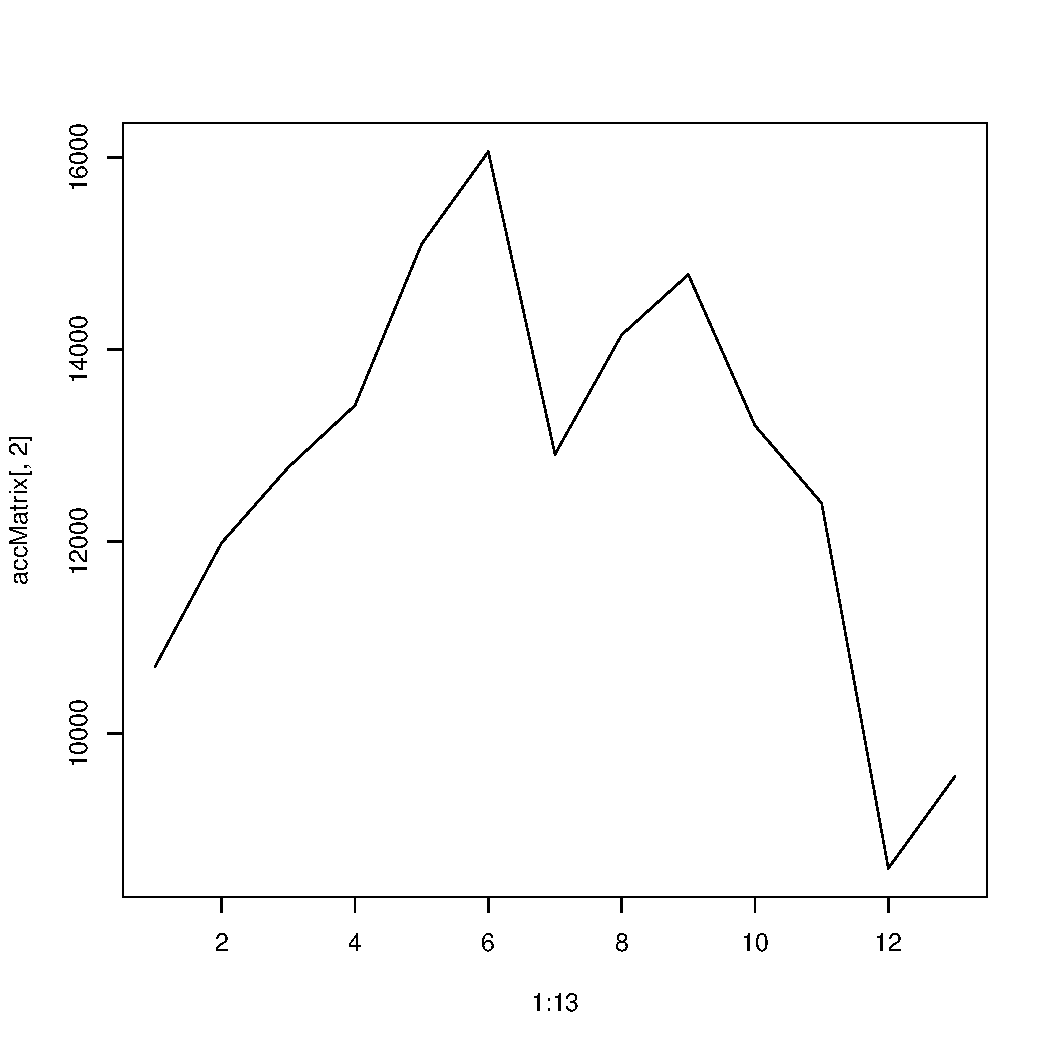
\includegraphics[width=0.33\textwidth]{../imagenes/segundoPeriodo.pdf}}
  \subfloat[Tercer periodo]{
   \label{f:periodo3}
    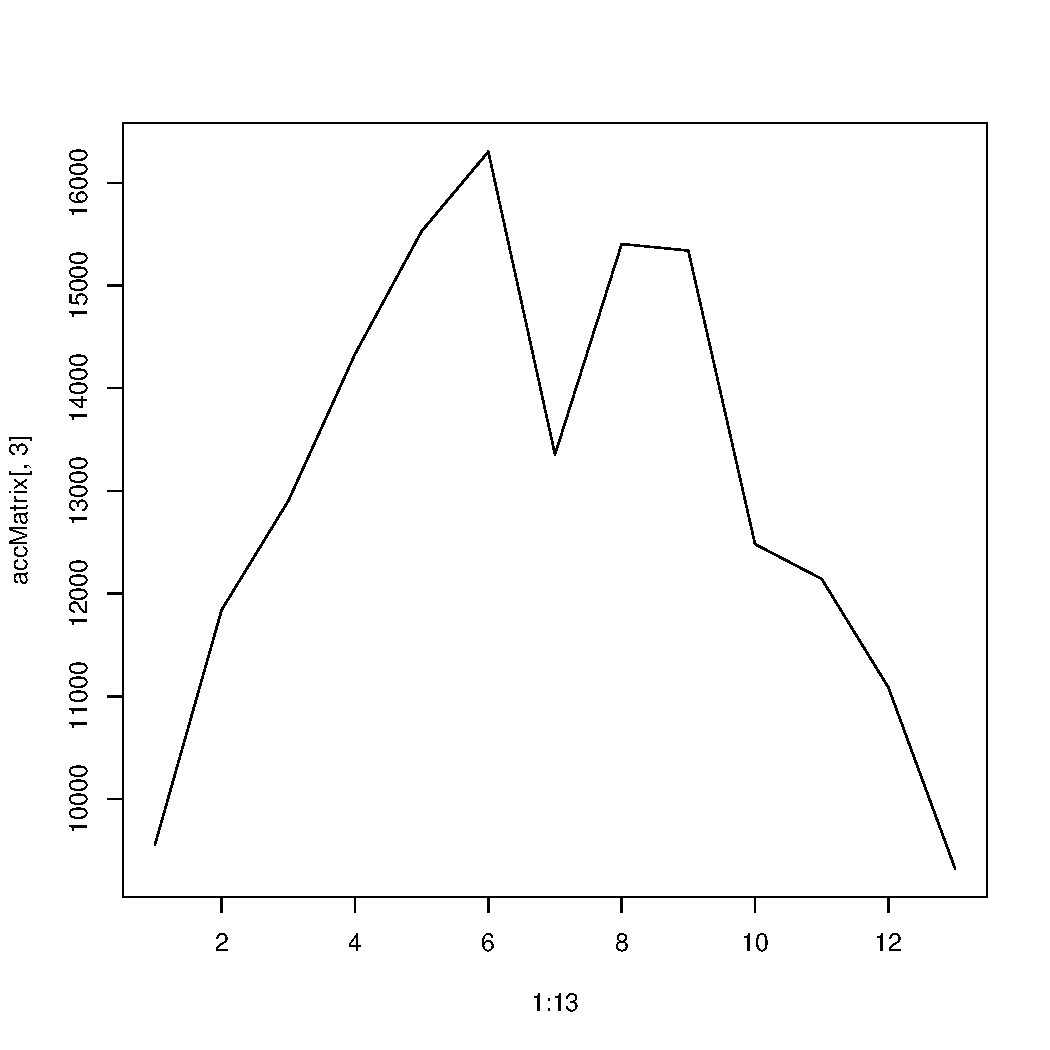
\includegraphics[width=0.33\textwidth]{../imagenes/tercerPeriodo.pdf}}
 \caption{Primeros periodos de la serie de accidentes en Italia}
 \label{f:periodos}
\end{figure}

\begin{figure}[]
 \centering
 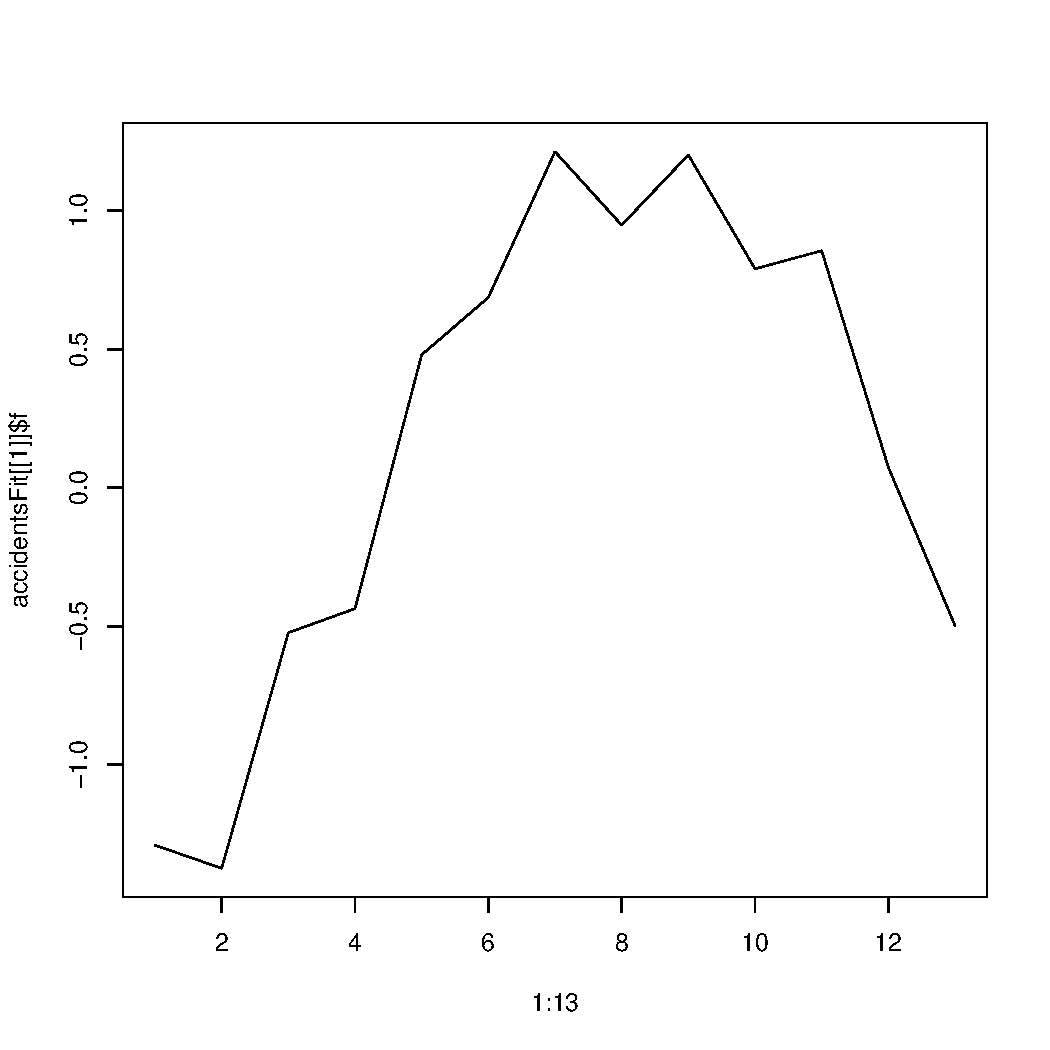
\includegraphics[width=0.5\textwidth]{../imagenes/accidentsComp.pdf}
 \caption{Componente principal dinámica para la serie de accidentes}
 \label{f:accidentsComp}
\end{figure}

En la figura \ref{f:accidentsComp} obtenemos por tanto un "patrón" del periodo de la serie original. Este patrón se obtiene en el intervalo $[-1, 1]$ y los valores de la serie original son mucho mayores, como se puede ver en la figura \ref{f:accidents}. Por esto, para restarle este patrón a la serie original se ha multiplicado el mismo, en cada intervalo periódico, por la media de la serie original en ese intervalo periódico antes de restarlo. El resultado se puede ver en la figura \ref{f:accidentsSinPatron}.

\begin{figure}[]
 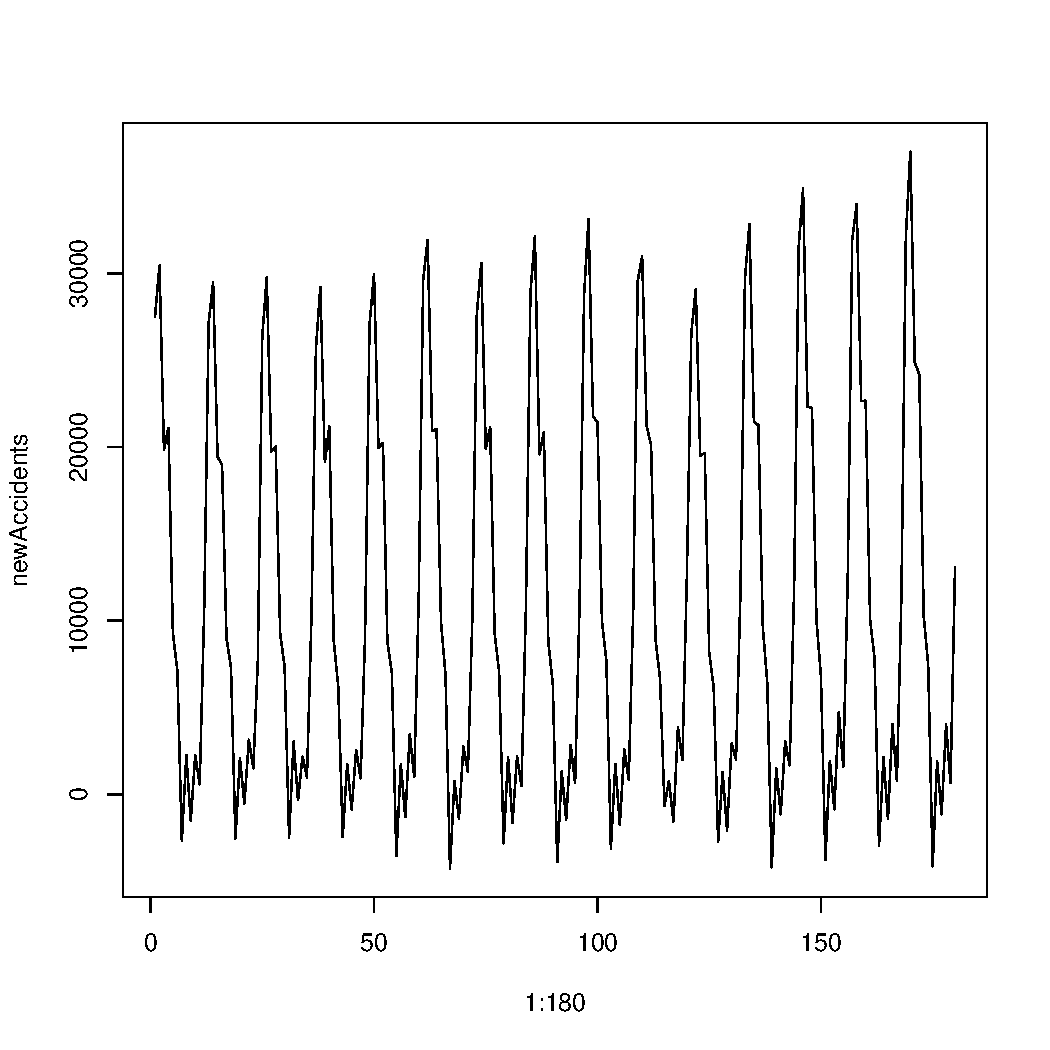
\includegraphics[width=\textwidth, height=0.4\textheight]{../imagenes/accidentsSinPatron.pdf}
 \caption{Serie de accidentes de coche en Italia sin patrón}
 \label{f:accidentsSinPatron}
\end{figure}

%TODO esto es así?


\section{Aplicación: Predicción de un conjunto de series temporales}

Como última aplicación, y quizás la más importante de todas las que hemos visto, vamos a ver si es posible predecir valores de un conjunto de series temporales a través de las componentes principales y las matrices de coeficientes $\beta$ y $\alpha$ que se obtienen con el método GDPC. La idea es la siguiente: supongamos que tenemos un conjunto de 100 series temporales, midiendo una información similar (por ejemplo, número de accidentes de coche mensuales en diferentes países) de los que queremos predecir los 5 siguientes valores de cada una de ellas. En lugar de tomar cada serie por separado y predecir sus siguientes 5 valores, vamos a obtener las componentes principales dinámicas, junto con sus coeficientes, y vamos a tratar cada componente principal como una nueva serie a la que le vamos a predecir sus próximos 5 valores. El número de componentes principales obtenidas será mucho menor que el número de series originales, por lo que el trabajo de predicción de nuevos valores será también mucho menor. Una vez tenemos los valores predichos de las componentes principales volvemos hacia atrás reconstruyendo los valores originales más los valores predichos con los coeficientes que habíamos sacado inicialmente con el método GDPC. Esto se puede hacer porque en la reconstrucción el único parámetro que depende de $T$, el número de valores en cada serie, es $\mathbf{f}$. Vamos a ver un pequeño ejemplo para verlo mejor. Recordemos que la reconstrucción con $k$ leads (que es equivalente a tener lags), $1 \leq j \leq m$, $1 \leq t \leq T$, está dada por
\begin{equation}\label{eq:recons}
	\widehat{z}_{j,t} = \sum_{i=0}^k \beta_{j,i+1}f_{t-i} + \alpha_j.
\end{equation}

Supongamos que inicialmente tenemos $m=3$ series de $T=5$ valores cada una y que obtenemos una única componente principal $\mathbf{f}$ obtenida con $k=4$ leads y que por tanto tendrá una longitud de $5+4=9$ valores, $\mathbf{f} = (f_1, f_2, \dots, f_9)$. Supongamos que queremos obtener los dos siguientes valores de las 3 series y para ello lo que hacemos es predecir los dos siguientes valores de $\mathbf{f}$, a los que vamos a llamar $\widehat{f}_{10}$ y $\widehat{f}_{11}$. Entonces definimos una extensión de $\mathbf{f}$, $\mathbf{\widehat{f}}$ como $\mathbf{\widehat{f}} = (f_1, \dots, f_9, \widehat{f}_{10}, \widehat{f}_{11})$ y vamos a realizar la reconstrucción dada por (\ref{eq:recons}) utilizando $\mathbf{\widehat{f}}$ en lugar de $\mathbf{f}$.\\

Entonces, si queremos reconstruir alguno de los valores originales de las series, no cambia nada. Por ejemplo, supongamos que queremos reconstruir $\widehat{z}_{3,5}$, entonces tenemos que,
\[	\widehat{z}_{3,5} = \beta_{3,1}f_5 + \beta_{3,2}f_6 + \beta_{3,3}f_7 + \beta_{3,4}f_8 + \beta_{3,5}f_9 + \alpha_3	\]

Ahora, podemos obtener también los valores $\widehat{z}_{1,6}$, $\widehat{z}_{2,6}$, $\widehat{z}_{3,6}$, $\widehat{z}_{1,7}$, $\widehat{z}_{2,7}$, $\widehat{z}_{3,7}$, que no estaban en las series originales, mediante las expresiones
\[	\widehat{z}_{1,6} = \beta_{1,1}f_6 + \beta_{1,2}f_7 + \beta_{1,3}f_8 + \beta_{1,4}f_9 + \beta_{1,5}\widehat{f}_{10} + \alpha_1	\]
\[	\widehat{z}_{2,6} = \beta_{2,1}f_6 + \beta_{2,2}f_7 + \beta_{2,3}f_8 + \beta_{2,4}f_9 + \beta_{2,5}\widehat{f}_{10} + \alpha_2	\]
\[	\widehat{z}_{3,6} = \beta_{3,1}f_6 + \beta_{3,2}f_7 + \beta_{3,3}f_8 + \beta_{3,4}f_9 + \beta_{3,5}\widehat{f}_{10} + \alpha_3	\]
\[	\widehat{z}_{1,7} = \beta_{1,1}f_7 + \beta_{1,2}f_8 + \beta_{1,3}f_9 + \beta_{1,4}\widehat{f}_{10} + \beta_{1,5}\widehat{f}_{11} + \alpha_1	\]
\[	\widehat{z}_{2,7} = \beta_{2,1}f_7 + \beta_{2,2}f_8 + \beta_{2,3}f_9 + \beta_{2,4}\widehat{f}_{10} + \beta_{2,5}\widehat{f}_{11} + \alpha_2	\]
\[	\widehat{z}_{3,7} = \beta_{3,1}f_7 + \beta_{3,2}f_8 + \beta_{3,3}f_9 + \beta_{3,4}\widehat{f}_{10} + \beta_{3,5}\widehat{f}_{11} + \alpha_3	\]

Esto tiene un inconveniente y es que a más valores intentemos predecir de $\mathbf{f}$ peor serán los valores obtenidos al hacer la reconstrucción porque los coeficientes, tanto los $\beta_{j,t}$ como los $\alpha_j$ se han generado con los valores conocidos de las series $z_{j,t}$ y no tienen por qué funcionar también para los valores predichos de $\mathbf{f}$. Sin embargo, este es un problema presente siempre que se trata la predicción de series temporales: a mayor horizonte de predicción, menos fiables son los resultados.\\

Para probar esto experimentalmente se han hecho un par de pruebas con el conjunto de datos \texttt{ipi91} disponible en el paquete \texttt{gdpc}. Concretamente, con las 4 primeras series, y utilizando 12 valores menos de los disponibles en cada serie para la obtención de las componentes principales dinámicas, para tener con qué comparar los valores predichos.

Se han cogido por tanto las series del IPI (Industrial Production Index) de Francia, Alemania, Italia y Reino Unido de los valores 1 al 252, se han metido en una matriz, por columnas, y se ha obtenido, con \texttt{k\_max = 10} y \texttt{expl\_var=0.95} una componente principal. Esta componente principal se ha modelado con un modelo AR(2) y con un modelo ARMA(2,2), obteniendo con cada uno de ellos los 5 siguientes valores. Después se ha hecho la reconstrucción de las series originales con los valores devueltos con el modelo AR(2) y los valores devueltos con el modelo ARMA(2,2) y en las figuras \ref{f:francia}, \ref{f:alemania}, \ref{f:italia} y \ref{f:uk} se pueden ver los últimos 100 valores de cada serie (incluyendo los 5 predichos).

\begin{figure}[]
 \centering
  \subfloat[Serie original]{
   \label{f:franciaO}
    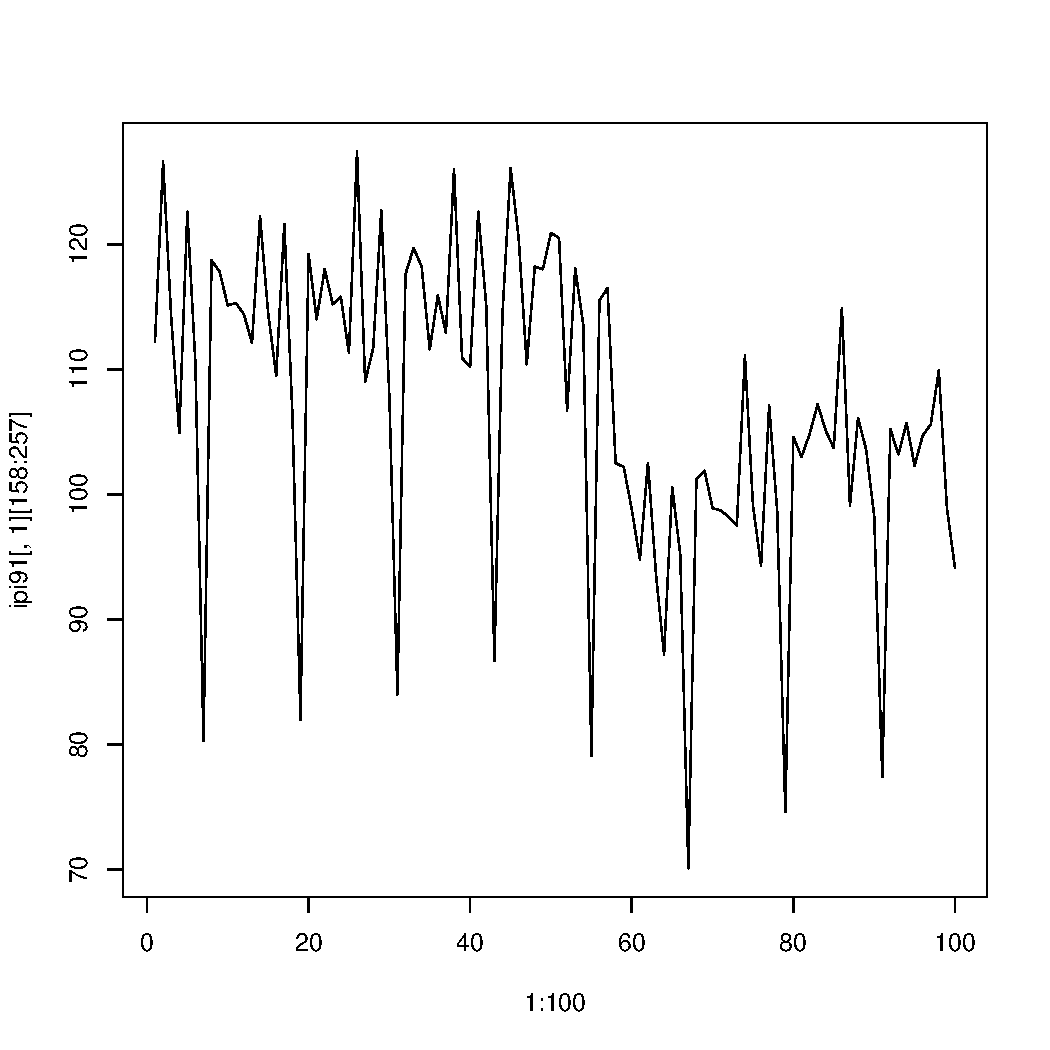
\includegraphics[width=0.5\textwidth]{../imagenes/ipi1original.pdf}}
  \subfloat[Reconstrucción con AR(2)]{
   \label{f:franciaAR}
    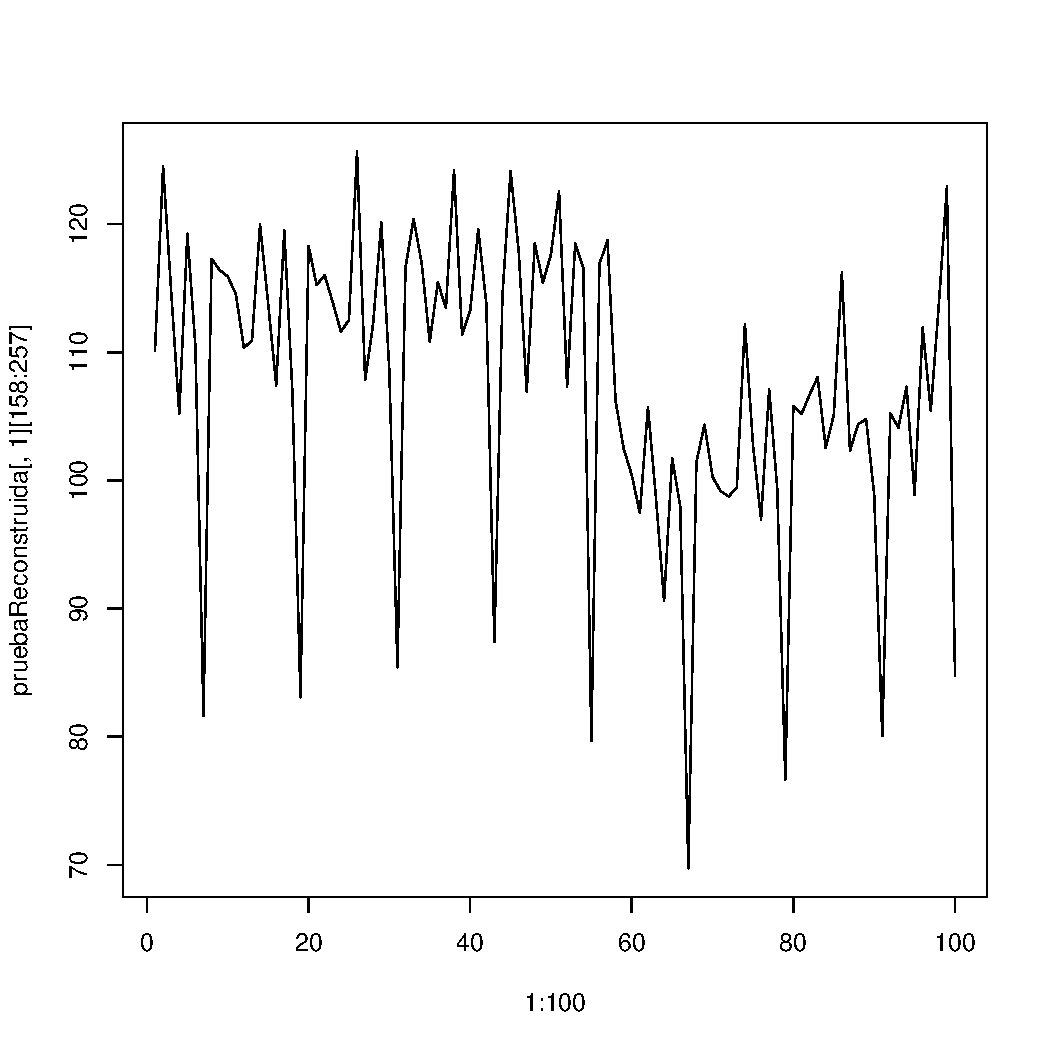
\includegraphics[width=0.5\textwidth]{../imagenes/ipi1ar.pdf}}
    \newline
  \subfloat[Reconstrucción con ARMA(2,2)]{
  \centering
   \label{f:franciaARMA}
    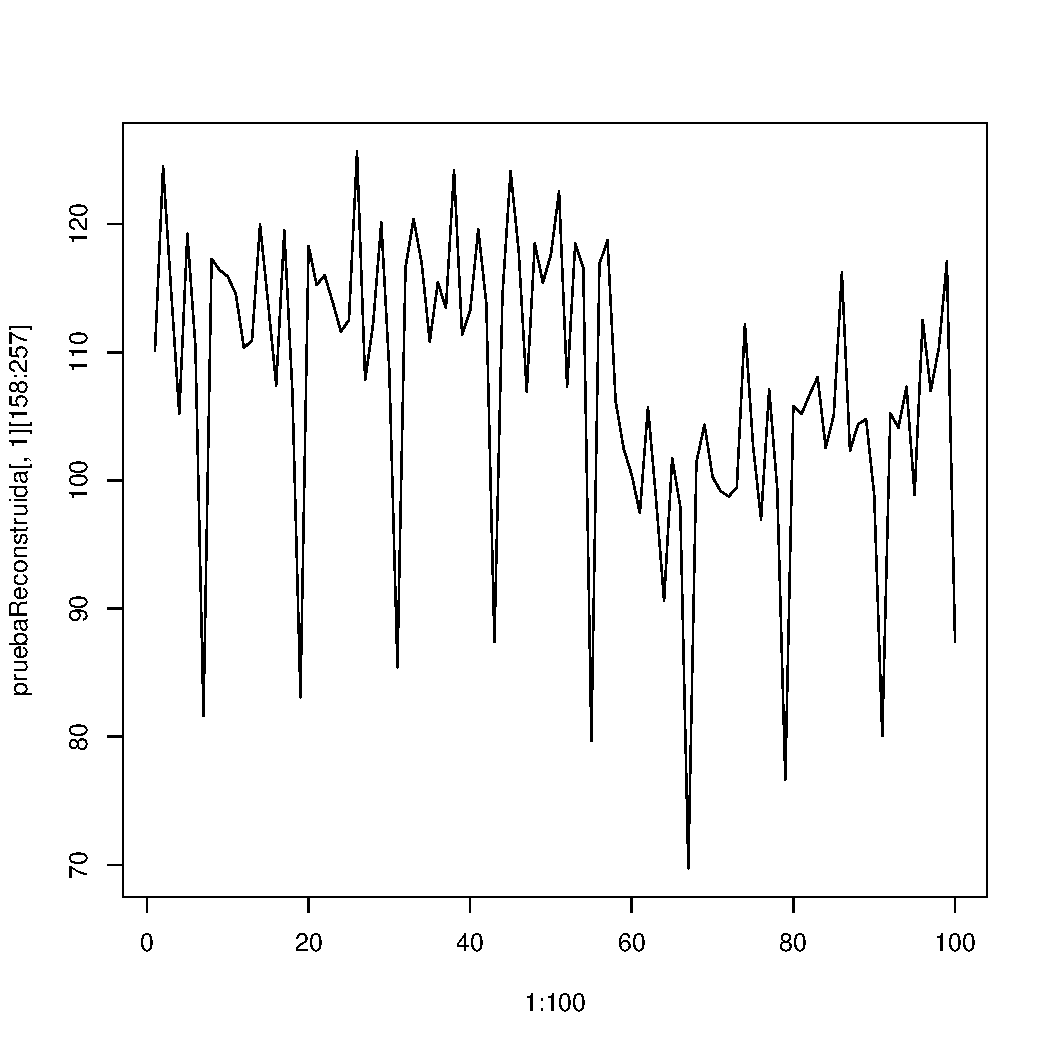
\includegraphics[width=0.5\textwidth]{../imagenes/ipi1arma.pdf}}
 \caption{IPI en Francia}
 \label{f:francia}
\end{figure}

\begin{figure}[]
 \centering
  \subfloat[Serie original]{
   \label{f:alemaniaO}
    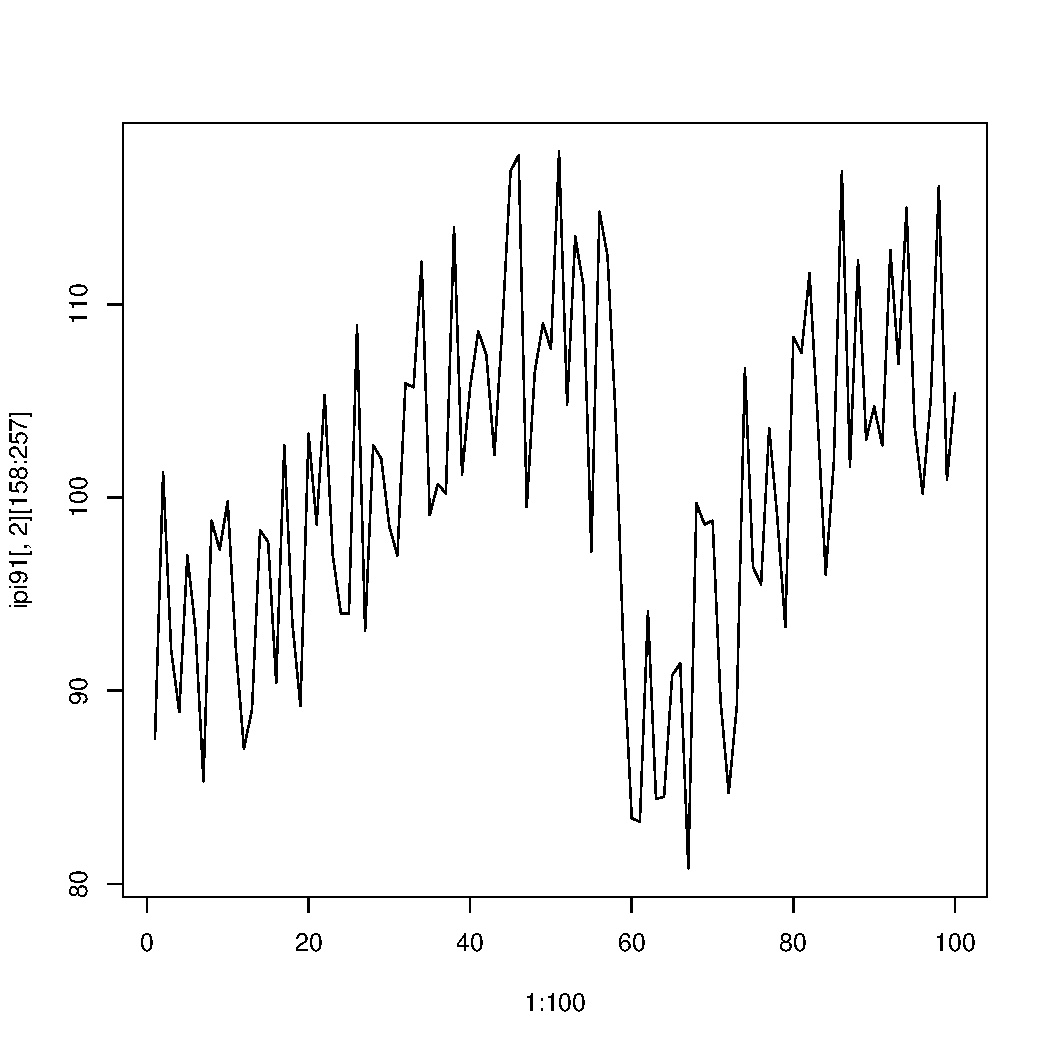
\includegraphics[width=0.5\textwidth]{../imagenes/ipi2original.pdf}}
  \subfloat[Reconstrucción con AR(2)]{
   \label{f:alemaniaAR}
    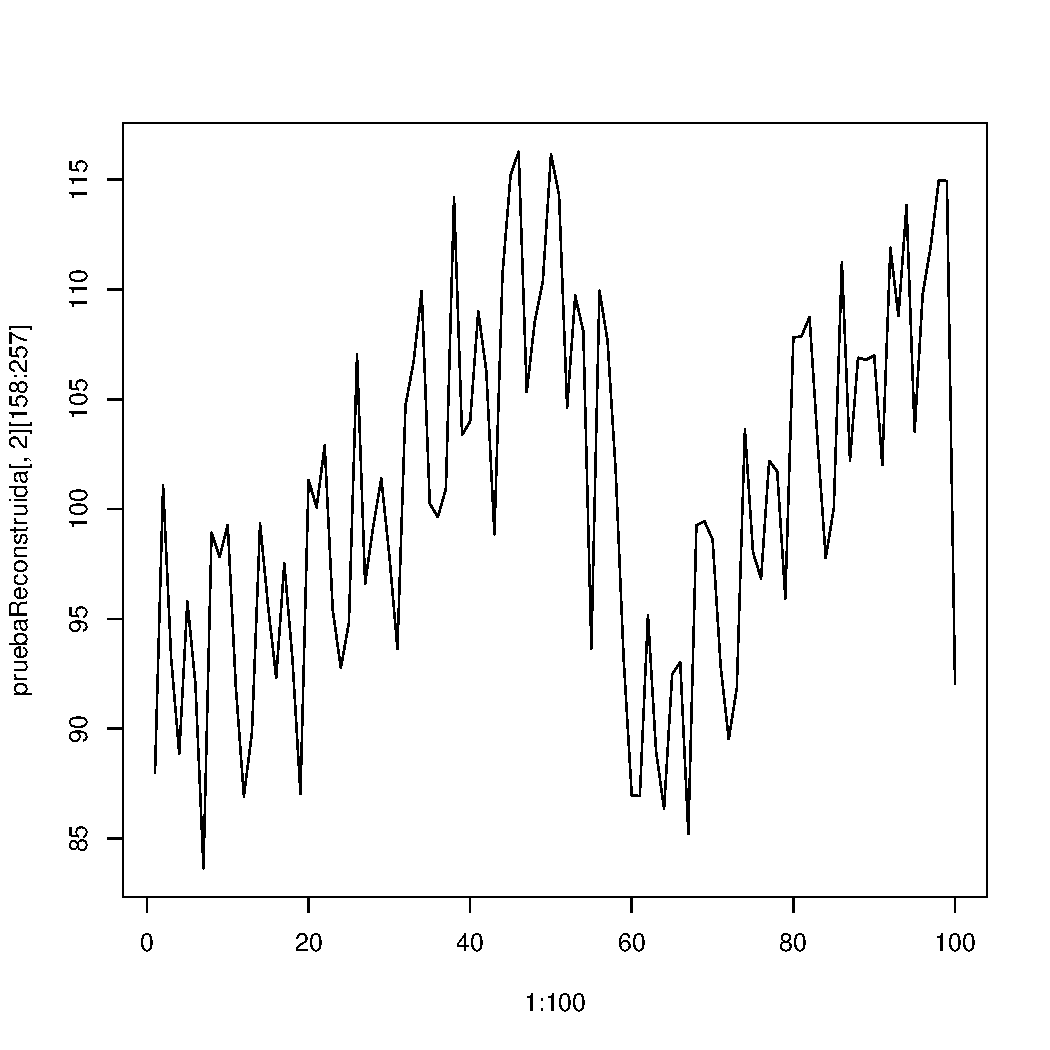
\includegraphics[width=0.5\textwidth]{../imagenes/ipi2ar.pdf}}
    \newline
  \subfloat[Reconstrucción con ARMA(2,2)]{
  \centering
   \label{f:alemaniaARMA}
    \includegraphics[width=0.5\textwidth]{../imagenes/ipi2arma.pdf}}
 \caption{IPI en Alemania}
 \label{f:alemania}
\end{figure}

\begin{figure}[]
 \centering
  \subfloat[Serie original]{
   \label{f:italiaO}
    \includegraphics[width=0.5\textwidth]{../imagenes/ipi3original.pdf}}
  \subfloat[Reconstrucción con AR(2)]{
   \label{f:italiaAR}
    \includegraphics[width=0.5\textwidth]{../imagenes/ipi3ar.pdf}}
    \newline
  \subfloat[Reconstrucción con ARMA(2,2)]{
  \centering
   \label{f:italiaARMA}
    \includegraphics[width=0.5\textwidth]{../imagenes/ipi3arma.pdf}}
 \caption{IPI en Italia}
 \label{f:italia}
\end{figure}

\begin{figure}[]
 \centering
  \subfloat[Serie original]{
   \label{f:ukO}
    \includegraphics[width=0.5\textwidth]{../imagenes/ipi4original.pdf}}
  \subfloat[Reconstrucción con AR(2)]{
   \label{f:ukAR}
    \includegraphics[width=0.5\textwidth]{../imagenes/ipi4ar.pdf}}
    \newline
  \subfloat[Reconstrucción con ARMA(2,2)]{
  \centering
   \label{f:ukARMA}
    \includegraphics[width=0.5\textwidth]{../imagenes/ipi4arma.pdf}}
 \caption{IPI en Reino Unido}
 \label{f:uk}
\end{figure}

En las imágenes apreciamos que el modelo ARMA(2,2) predice la serie un poco mejor que el modelo AR(2). En el caso del modelo AR(2), en la serie del IPI en Francia, se obtiene una diferencia, en valor del absoluto, entre los valores predichos y los originales, de 7.25 en el primer valor predicho, 0.16 en el segundo, 3.85 en el tercero, 24.02 en el cuarto y 9.35 en el quinto. En el caso del modelo ARMA(2,2), estas diferencias son de 7.84, 1.4, 0.44, 18.23 y 6.68. Efectivamente el modelo ARMA(2,2) tiene menos error en esta serie que el modelo AR(2) y vemos que, en general, según vamos aumentando el horizonte de predicción el error va aumentando. Los errores por encima de 10 se consideran altos puesto que los valores de la serie oscilan entre 85 y 115.\\

Para la serie del IPI en Alemania, las diferencias con el modelo AR(2) son de 9.57 en el primer valor predicho, 6.87 en el segundo, 1.12 en el tercero, 14.05 en el cuarto y 13.35 en el quinto. En el caso del modelo ARMA(2,2), las diferencias son de 8.09, 4.05, 4.31, 10.58 y 13.08. En este caso ambos modelos están más igualados pero de nuevo se ve que según se aumenta el horizonte de predicción hay más error.\\

En este caso experimental se han usado modelos sencillos y lineales, pero convendría usar modelos más potentes para obtener unas buenas predicciones de la serie $\mathbf{f}$ y que así los errores en la predicción al volver hacia las series originales se redujeran, siempre teniendo en cuenta que son reconstrucciones utilizando las componentes principales dinámicas, es decir, que se está llevando a cabo una reducción de dimensión con la consiguiente pérdida de información, con lo que siempre va haber un error de base, más allá del que se cometa en la predicción.




%\end{document}

%
\chapter{Conclusiones y vías futuras}
\label{ch:conclusiones}

A partir del estudio realizado en este trabajo se pueden sacar las siguientes conclusiones:
\begin{enumerate}
\item El número de posibles aplicaciones al artículo de Peña y Yohai en \cite{pena16} son amplias y aquí se han tratado sólo unas cuantas, pero sería interesante seguir profundizando en el estudio.
\item Como habíamos previsto, la aplicación a compresión de imágenes no nos ha dado un nuevo método real que se pueda utilizar en compresión de imágenes por el tiempo que se tarda en obtener las componentes principales y la relativa calidad de las imágenes reconstruidas, pero se han obtenido resultados mejores a los esperados inicialmente en cuanto a calidad y ha servido para el propósito principal que tenía: entrar en contacto con el paquete de R que implementa el GDPC y entender mejor el método, así como ver qué cantidad de compresión puede llegar a haber perdiendo en realidad poca información.
\item Se han cumplido de esta forma 3 de los 4 objetivos previstos inicialmente.
\end{enumerate}

Existen dos posibles vías de desarrollo a partir de este momento:
\begin{enumerate}
\item Profundizar en la aplicación de búsqueda de patrones, llegando a dividir una serie en sus distintos elementos e intentando utilizar también el procedimiento GDPC para obtener otros de estos elementos, como la tendencia de la serie.
\item Profundizar en la aplicación de predicción de nuevos valores de un gran conjunto de series a través de la predicción de nuevos valores de las componentes principales dinámicas, haciendo incapié en la utilización de mejores modelos para la predicción de las mismas, utilizando más modelos lineales y no lineales, que no se ha tratado aquí por no ser el tema principal del trabajo.
\end{enumerate}




%
%%\nocite{*}
%\begin{thebibliography}{99}

%\bibitem{JAPSHA11}
%  Nathalie Japkowicz, Mohak Shah,
%  \emph{Evaluating Learning Algorithms - A Classification Perspective},
%  Cambridge University Press,
%  2011.

%\bibliographystyle{unsrt}
%\bibliography{bibliografia}{}

\end{thebibliography}
%
%\appendix
%\input{apendices/manual_usuario/manual_usuario}
%%\input{apendices/paper/paper}
%\input{glosario/entradas_glosario}
% \addcontentsline{toc}{chapter}{Glosario}
% \printglossary
\chapter*{}
\thispagestyle{empty}

\bibliography{capitulos/bibliografia}
\label{bibliography}
\bibliographystyle{plain}

\end{document}
